\part{圆}
\section{基本性质}
\begin{definition}[圆]
    平面内围绕一个定点 $O$ 并以一定长度 $r$ 为距离旋转一周所形成的封闭曲线叫做圆(Circle)。
    \newline
    定点$O$称作圆心,$r$称作圆的半径。圆是到定点O的距离等于定长r的点的集合。\\
    (1) 半径: 连接圆心和圆上任意一点的线段叫做半径,字母表示为r。\\
    (2) 直径: 通过圆心并且两端都在圆上的线段叫做直径,字母表示为d。直径所在的直线是圆的对称轴。\\
    (3) 弦:连接圆上任意两点的线段叫做弦,在同一个圆内最长的弦是直径。\\
    (4) 弧: 圆上任意两点间的部分叫做圆弧,简称弧,符号表示为$\overset{\frown}{AB}$。大于半圆的弧称为优弧,例如$\overset{\frown}{ADB}$;小于半圆的弧称为劣弧,如$\overset{\frown}{AB}$。同一圆中能够互相重合的两条弧叫做等弧。\\
    (5) 任意定点及定长可以构成一个圆。圆心和半径同时相同的圆为同圆,圆心相同半径不同的圆称作同心圆,半径相同圆心不同的圆称作等圆。\\
\end{definition}

\begin{figure}[H]
    \centering
    \includegraphics[width=0.8\linewidth]{figures/圆.png}
\end{figure}


\newpage 
\section{垂径定理}
\begin{theorem}[垂径定理]
圆具有旋转不变性以及对称性。垂直于弦的直径平分这条弦,且平分弦所对的两条弧。
\end{theorem}
\begin{figure}[H]
    \centering
    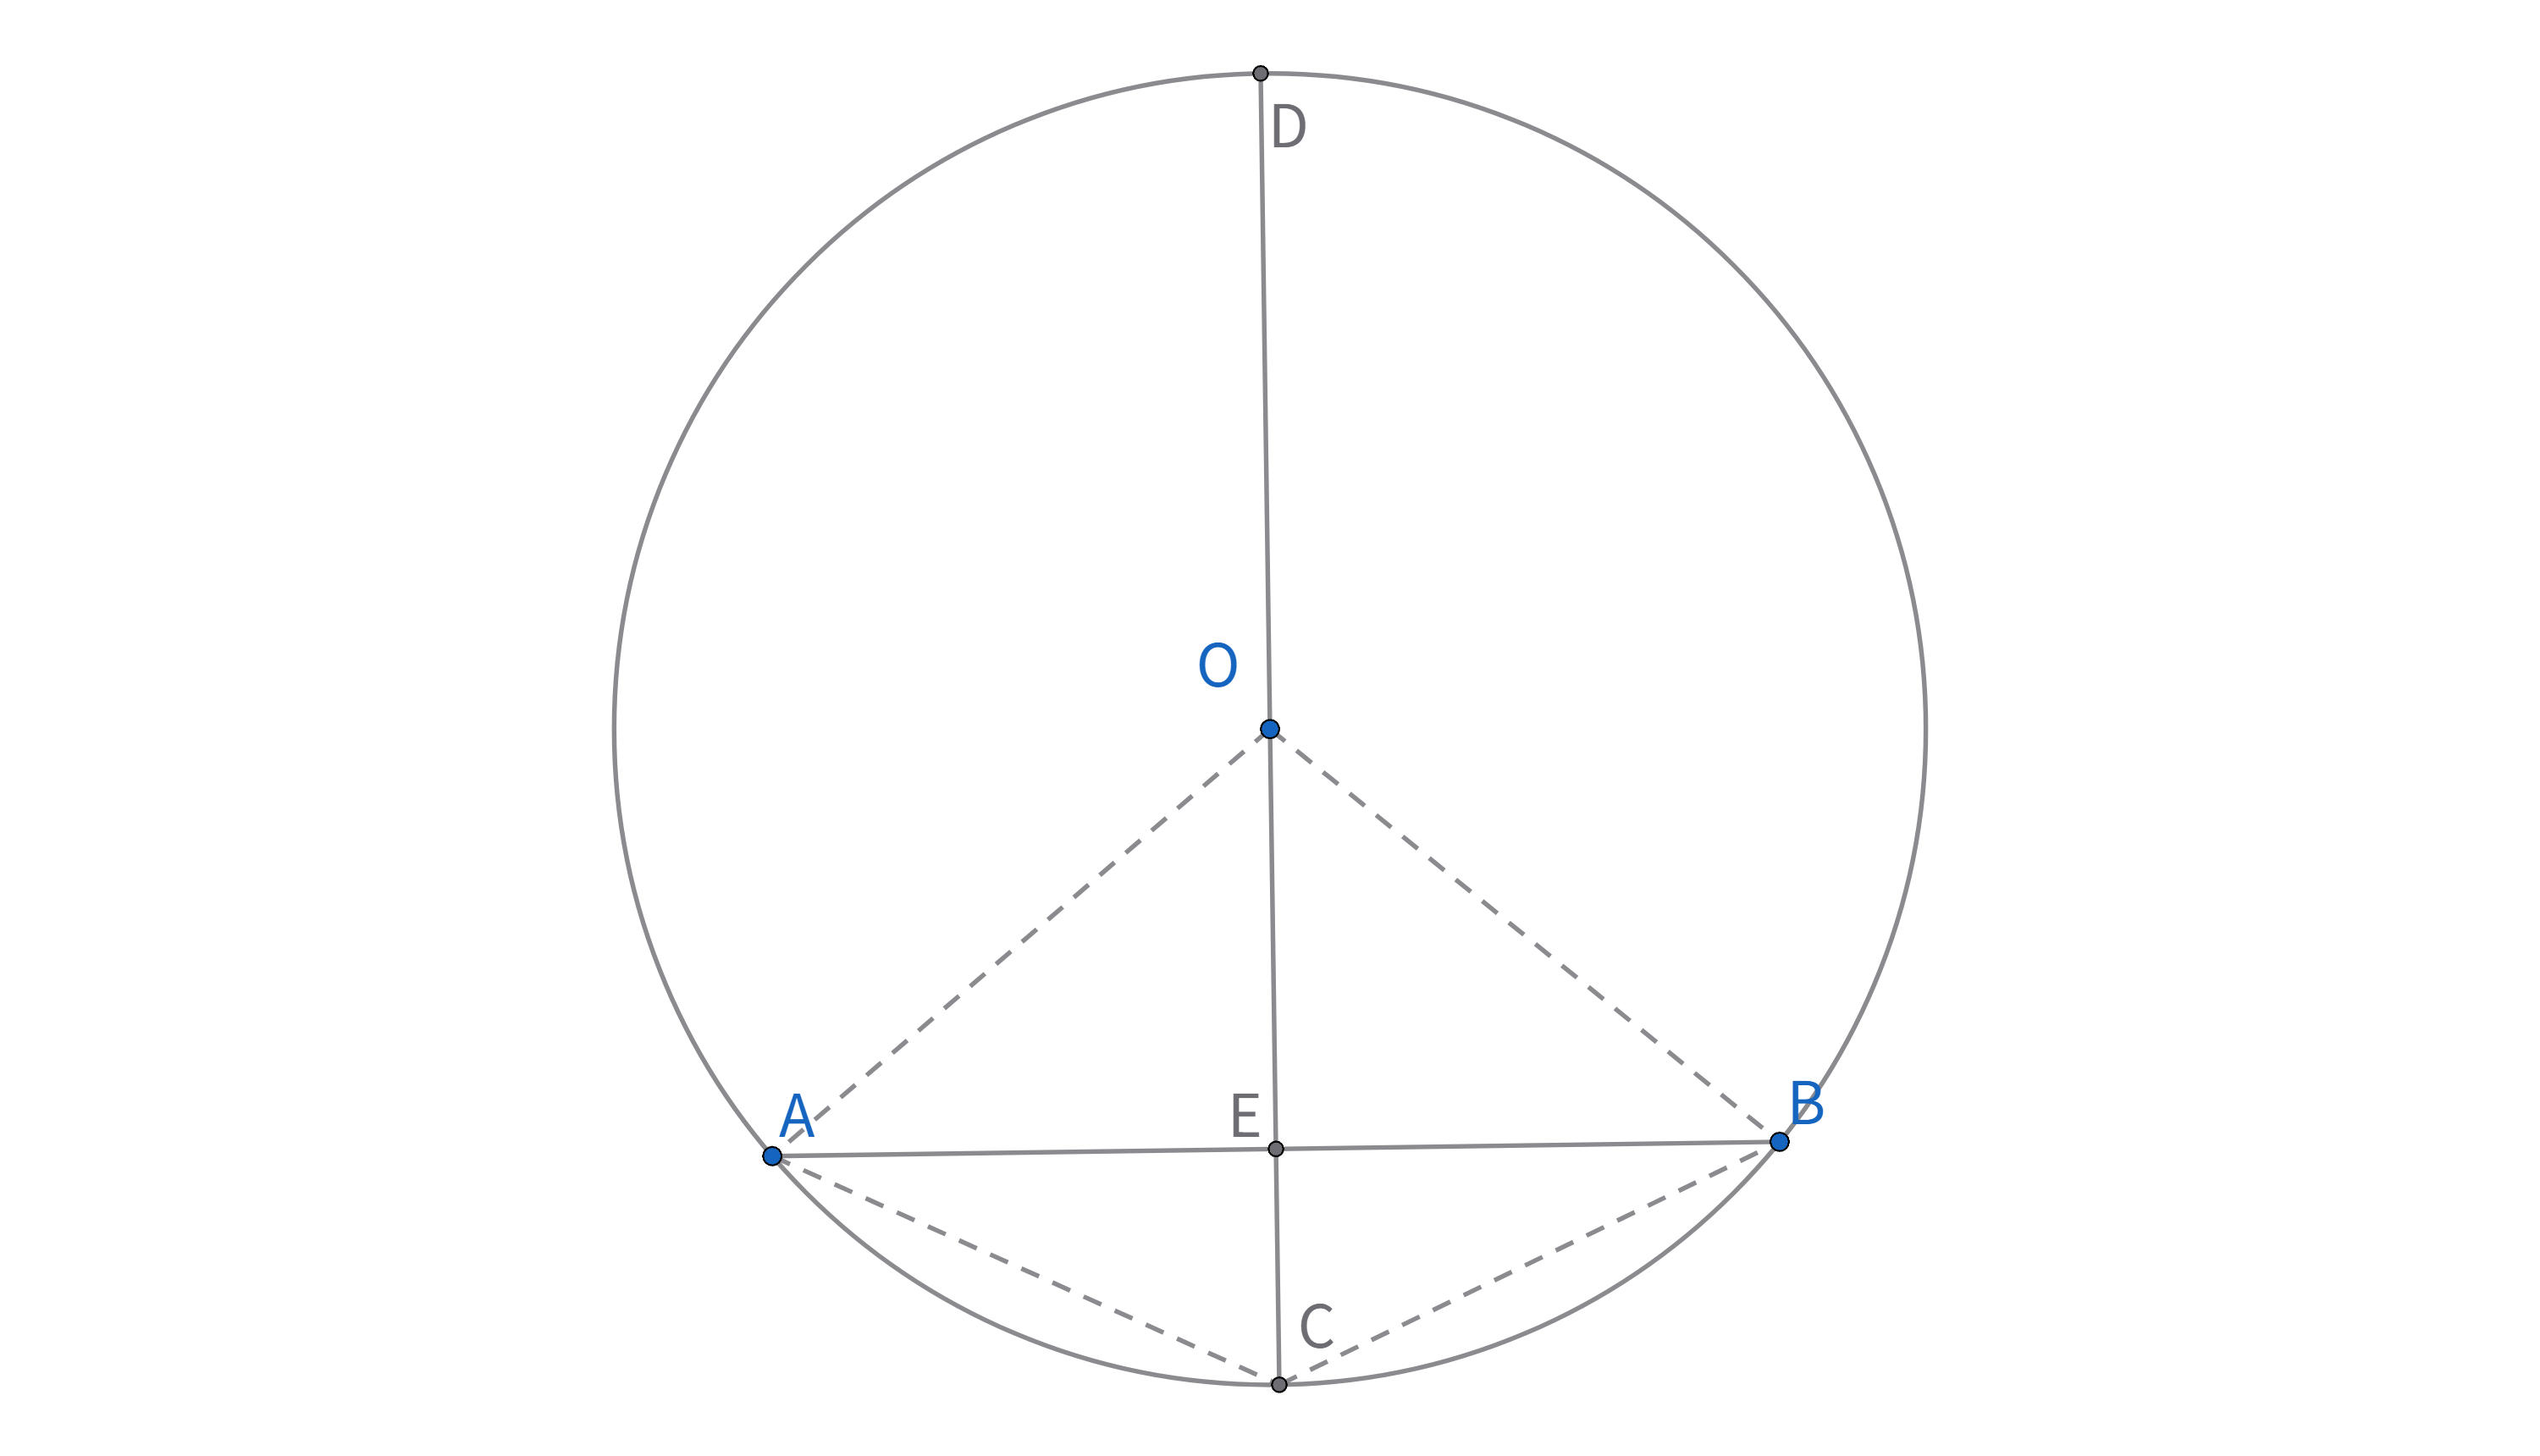
\includegraphics[width=\linewidth]{figures/垂径定理.png}
    \caption{垂径定理}
    % \label{fig:enter-label}
\end{figure}


\newpage 
\section{圆周角定理}
\begin{theorem}[圆周角定理]
    对任意一条弦,与圆心构成的顶角称作圆心角,与圆周上另一点构成的顶角叫做圆周角。圆内的圆周角具有如下性质:
    
    (1) 直径所对圆周角为90度。
    
    (2) 同弧所对圆周角度数是圆心角的一半。
    
    (3) 同弧或等弧所对圆周角度数相等。

    (4) 弦分割的两圆弧所对圆周角互补。
\end{theorem}
\begin{figure}[H]
    \centering
    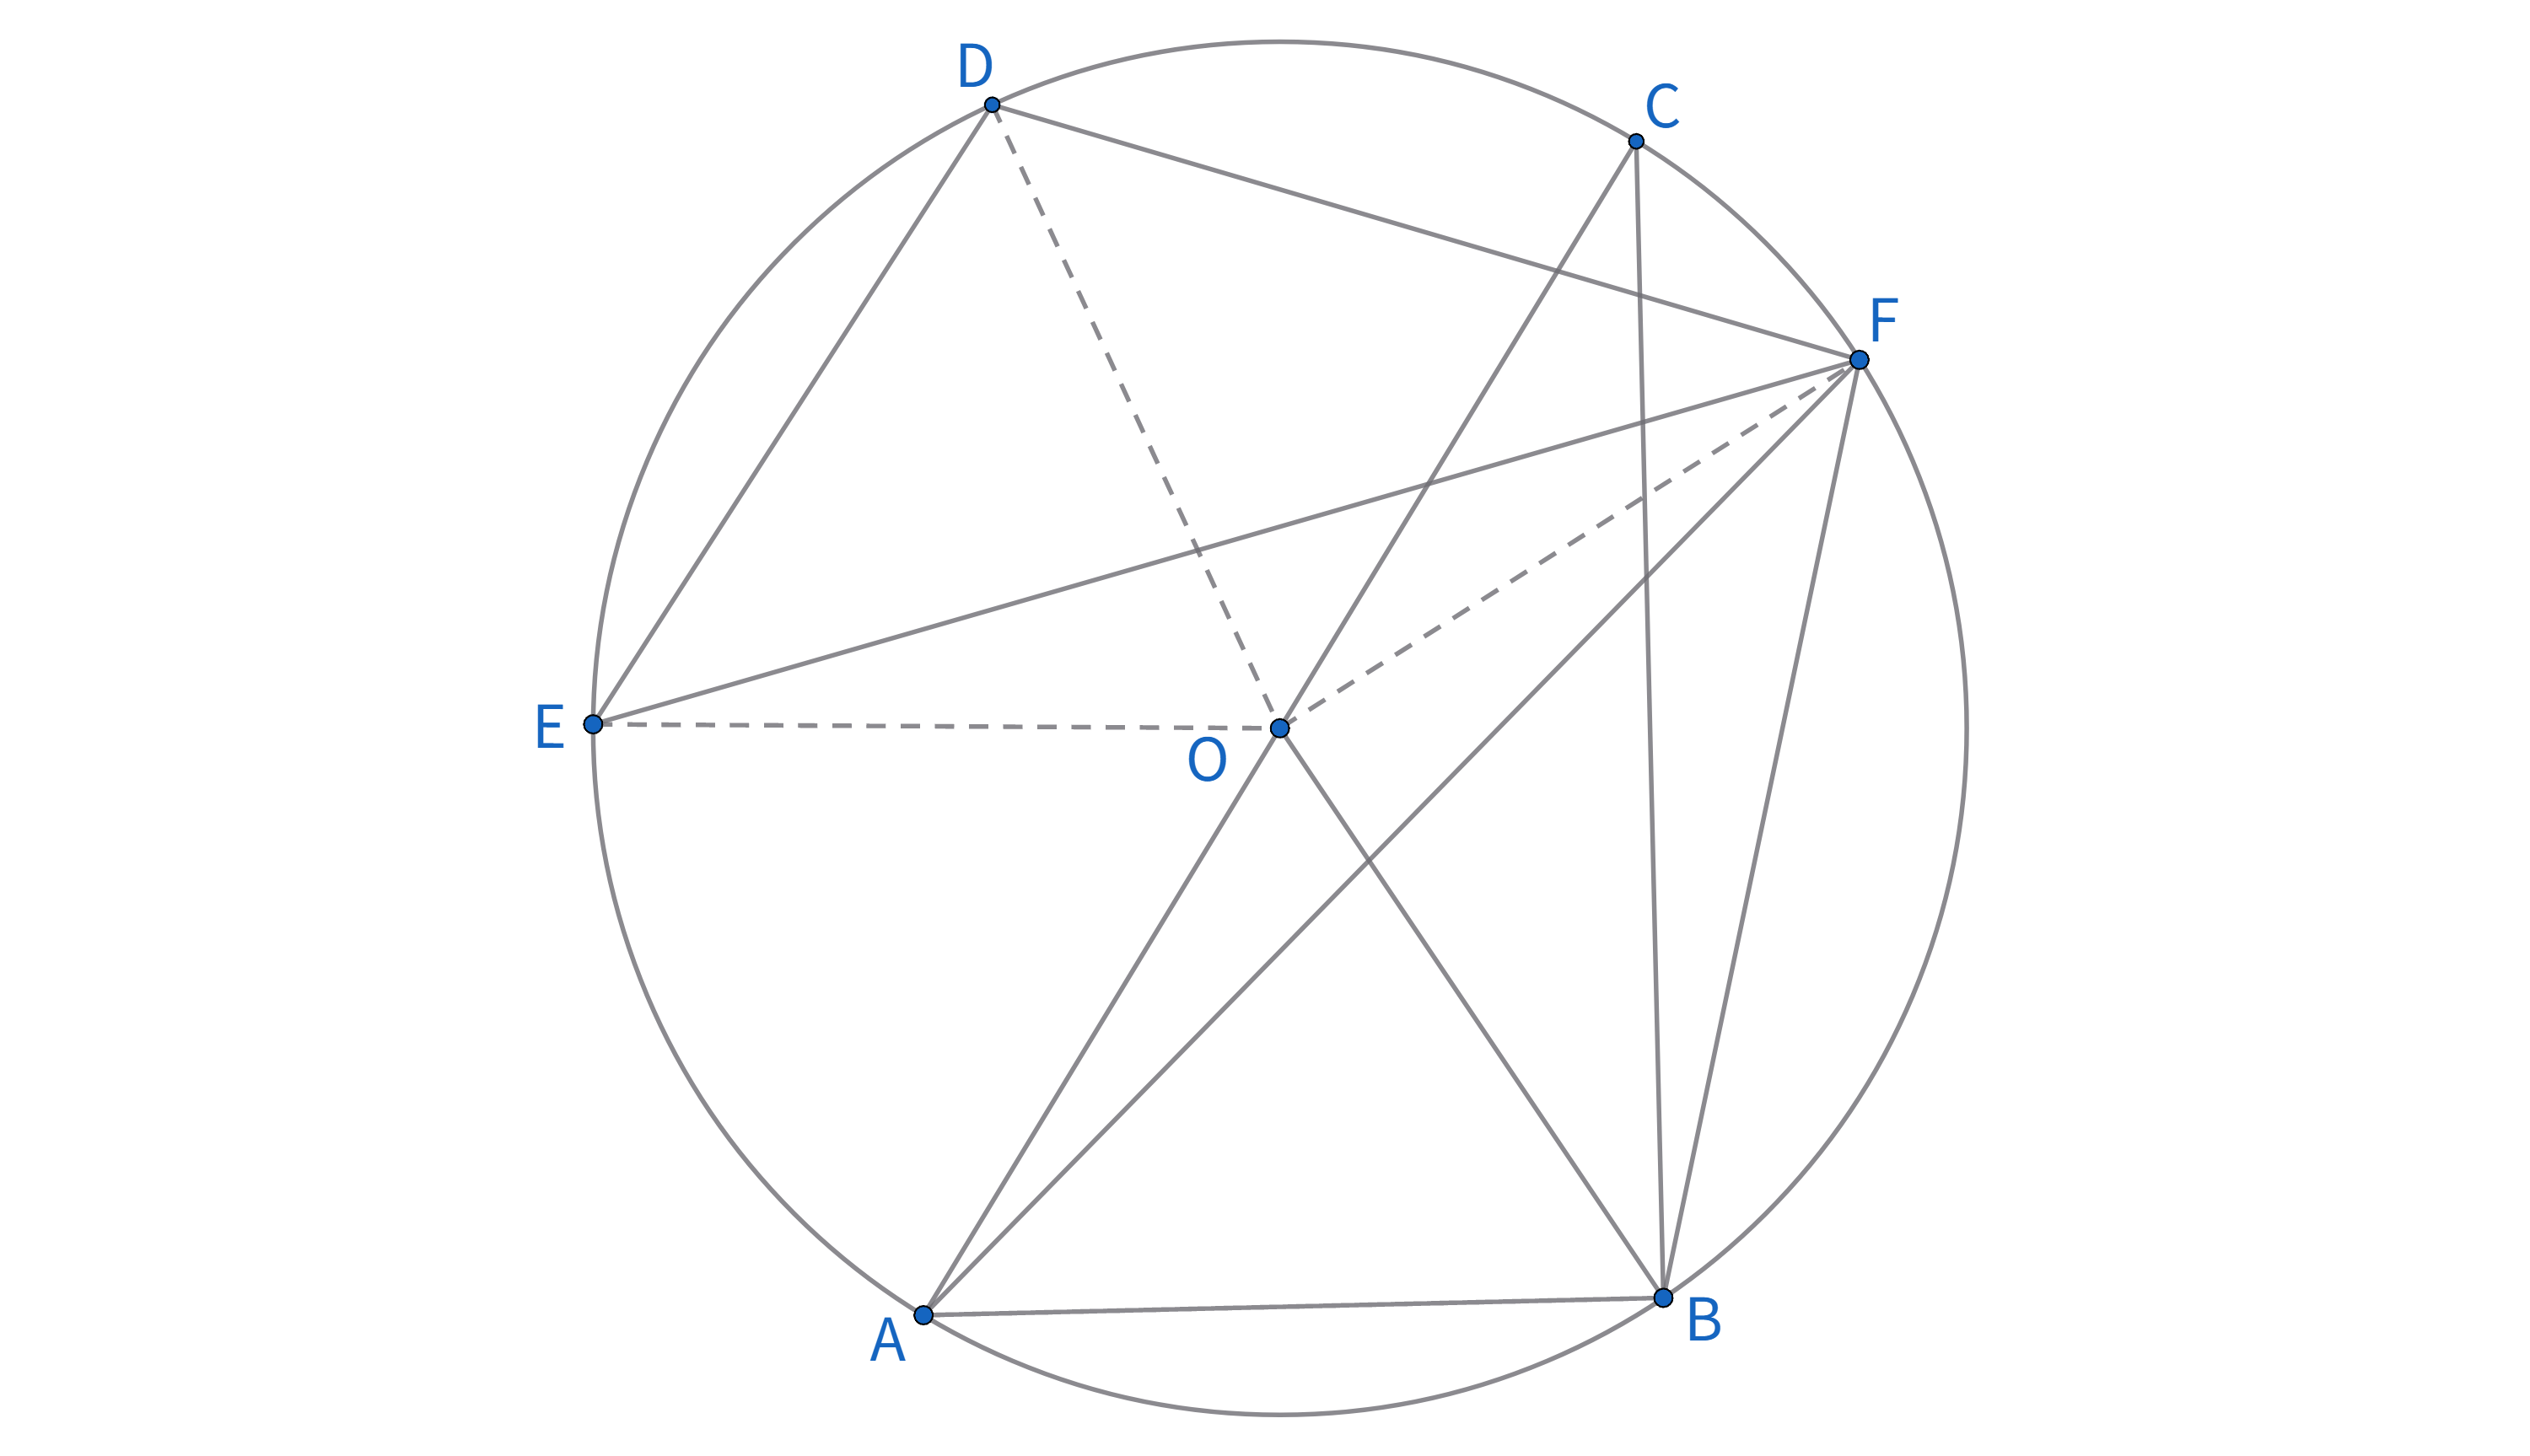
\includegraphics[width=0.8\linewidth]{figures/圆周角定理.png}
    \caption{圆周角定理}
    % \label{fig:enter-label}
\end{figure}
\begin{figure}[H]
    \centering
    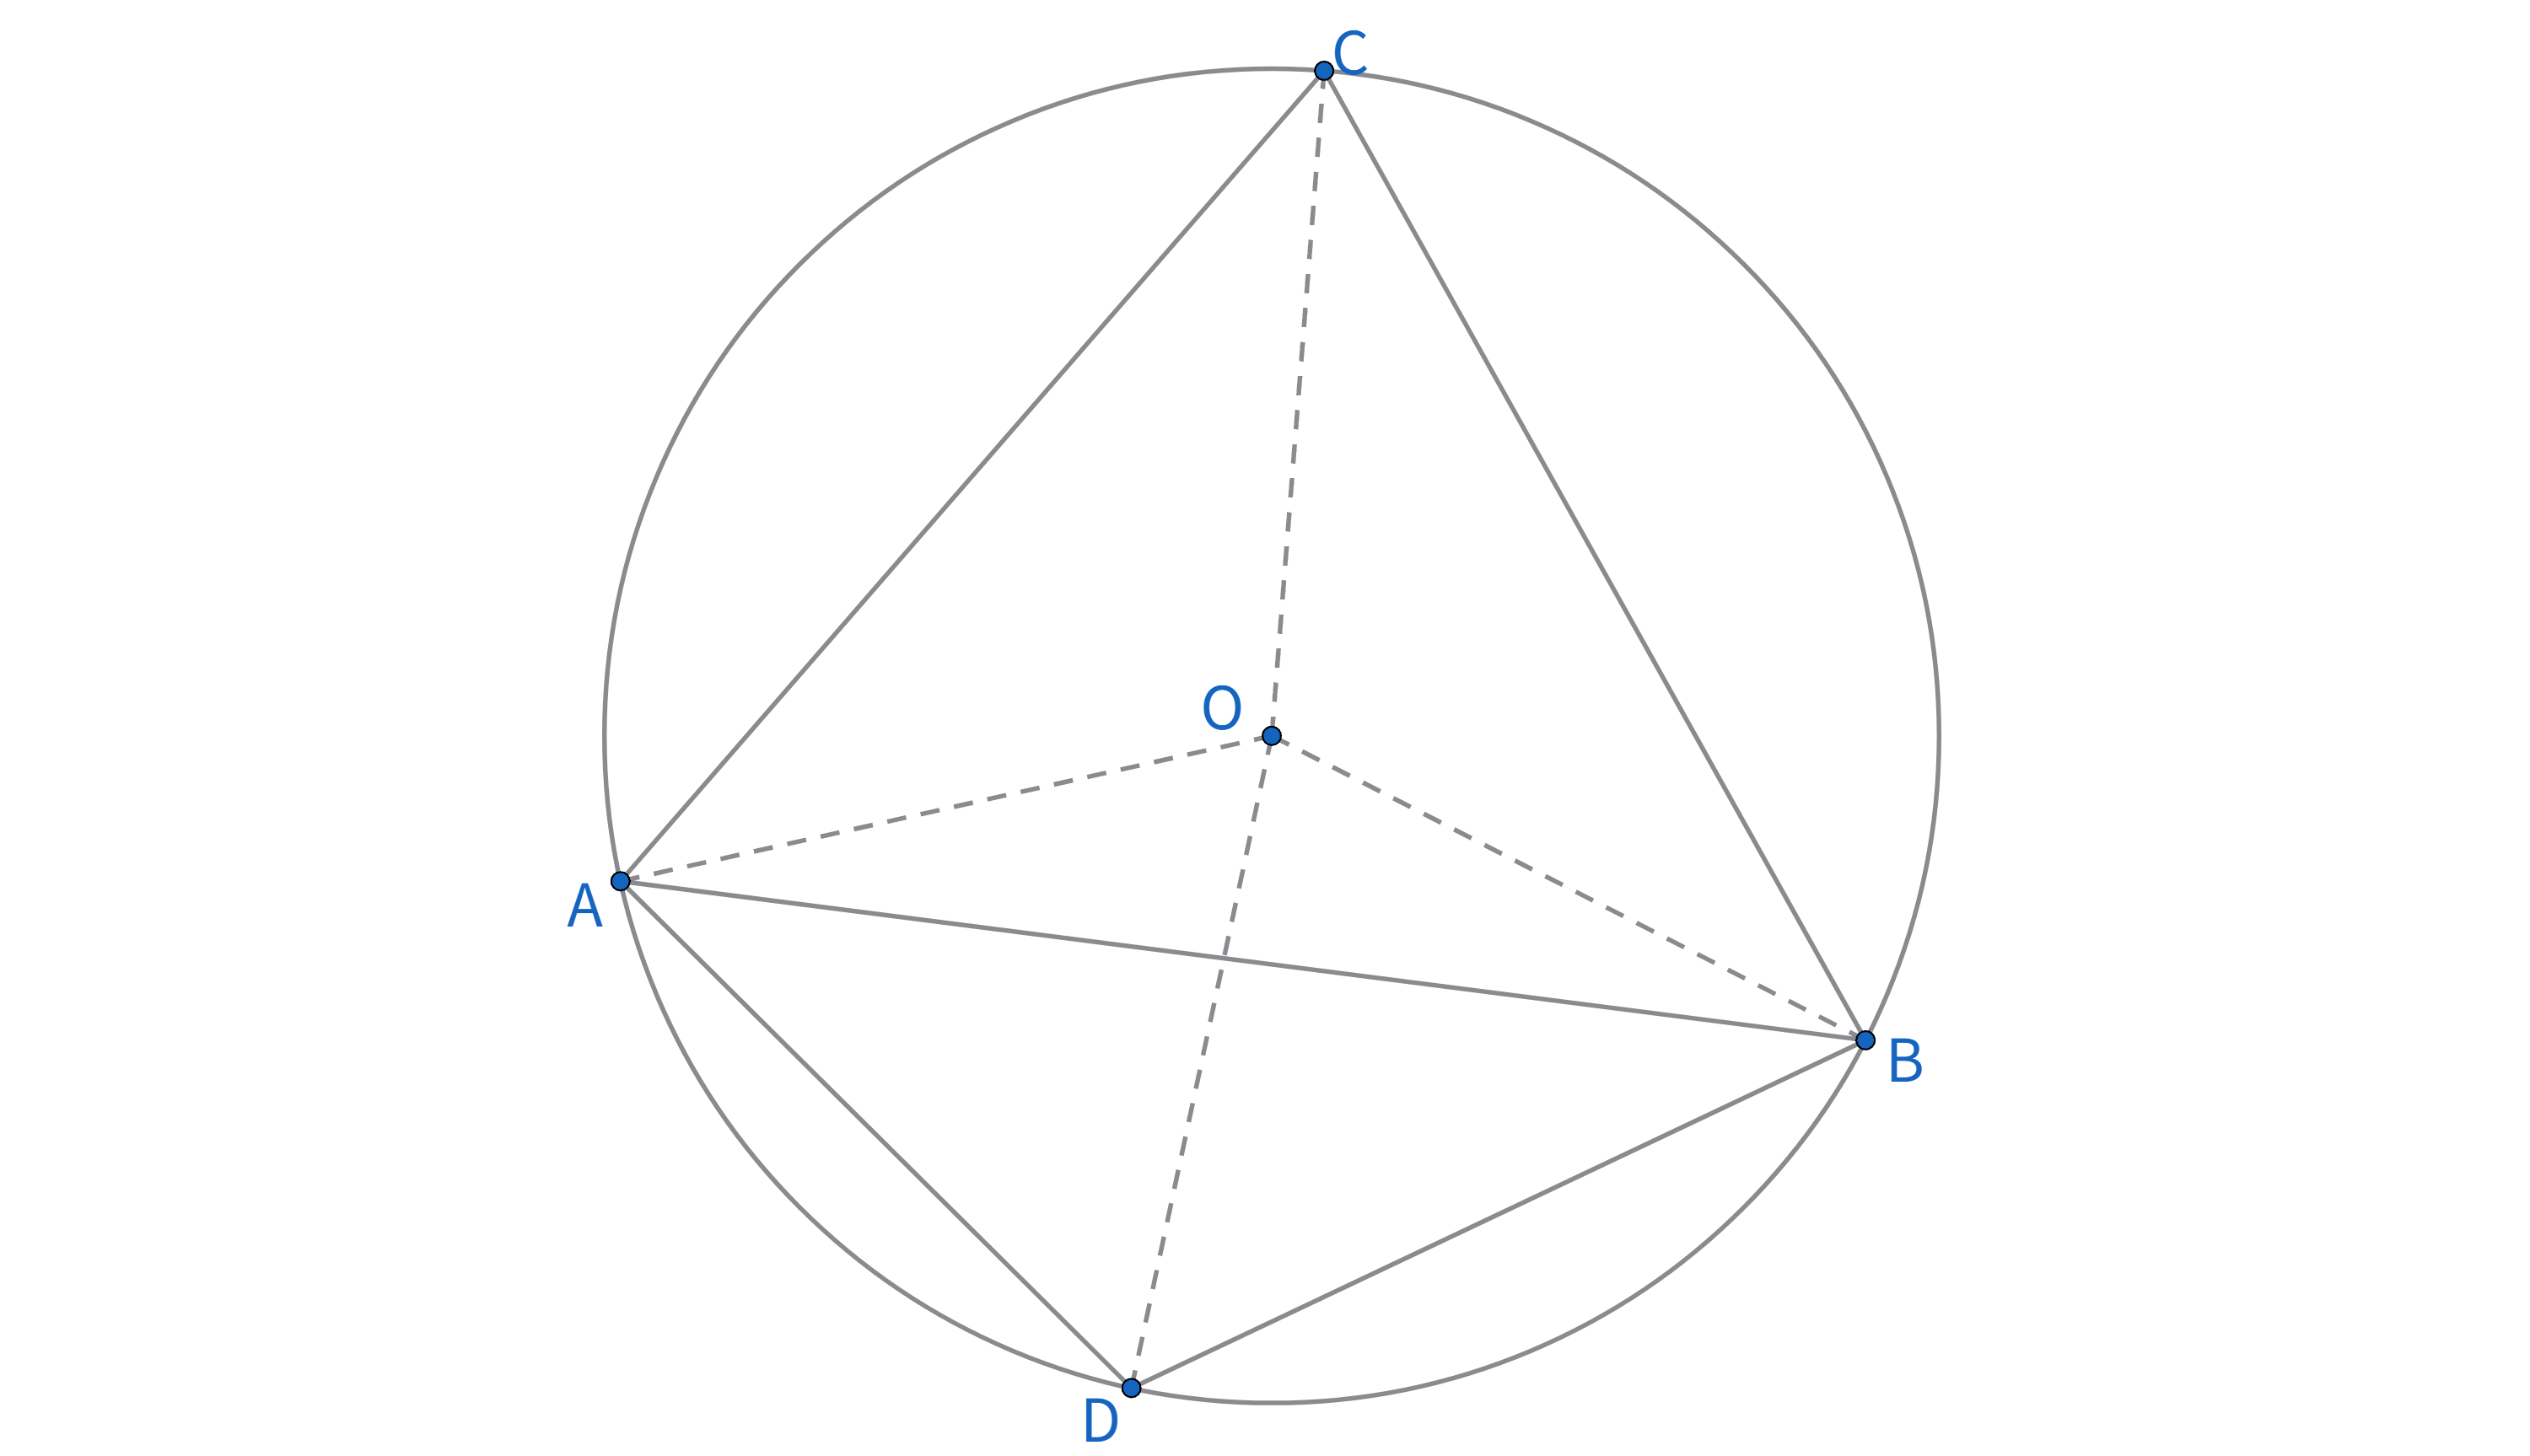
\includegraphics[width=0.8\linewidth]{figures/圆周角定理-对角互补.png}
    \caption{对角互补}
    % \label{fig:enter-label}
\end{figure}


\begin{exercise}
设 $\triangle ABC$ 是一个锐角三角形,外心为 $O$,点 $K$ 满足 $KA$ 与外接圆 $(ABC)$ 相切,并且 $\angle KCB = 90^\circ$。点 $D$ 在 $\overline{BC}$ 上,满足 $KD \parallel AB$。证明:直线 $DO$ 经过点 $A$。
\end{exercise}



\begin{exercise}
在 $\triangle ABC$ 中,射线 $AO$ 交 $BC$ 于 $D$,点 $K$ 满足 $KA$ 与圆 $(ABC)$ 相切,而且 $\angle KCB = 90^\circ$。证明:$KD \parallel AB$。
\end{exercise}



\begin{exercise}
不等边 $\triangle ABC$ 中,设 $K$ 是 $\angle A$ 的平分线与 $BC$ 的垂直平分线的交点。证明:$A, B, C, K$ 四点共圆。
\end{exercise}


\newpage 
\section{点与圆的位置关系}
用$d(A,B)$表示两点A和B的距离,点与圆的关系可分为三类。
\begin{itemize}
    \item 点在圆外:当点A与圆心O的距离大于半径r时,即$d(A,O) > r$。
    \item 点在圆上:当点A与圆心O的距离等于半径r时,即$d(A,O) = r$。
    \item 点在圆内:当点A与圆心O的距离小于半径r时,即$d(A,O) < r$。
\end{itemize}
\begin{figure}[H]
    \centering
    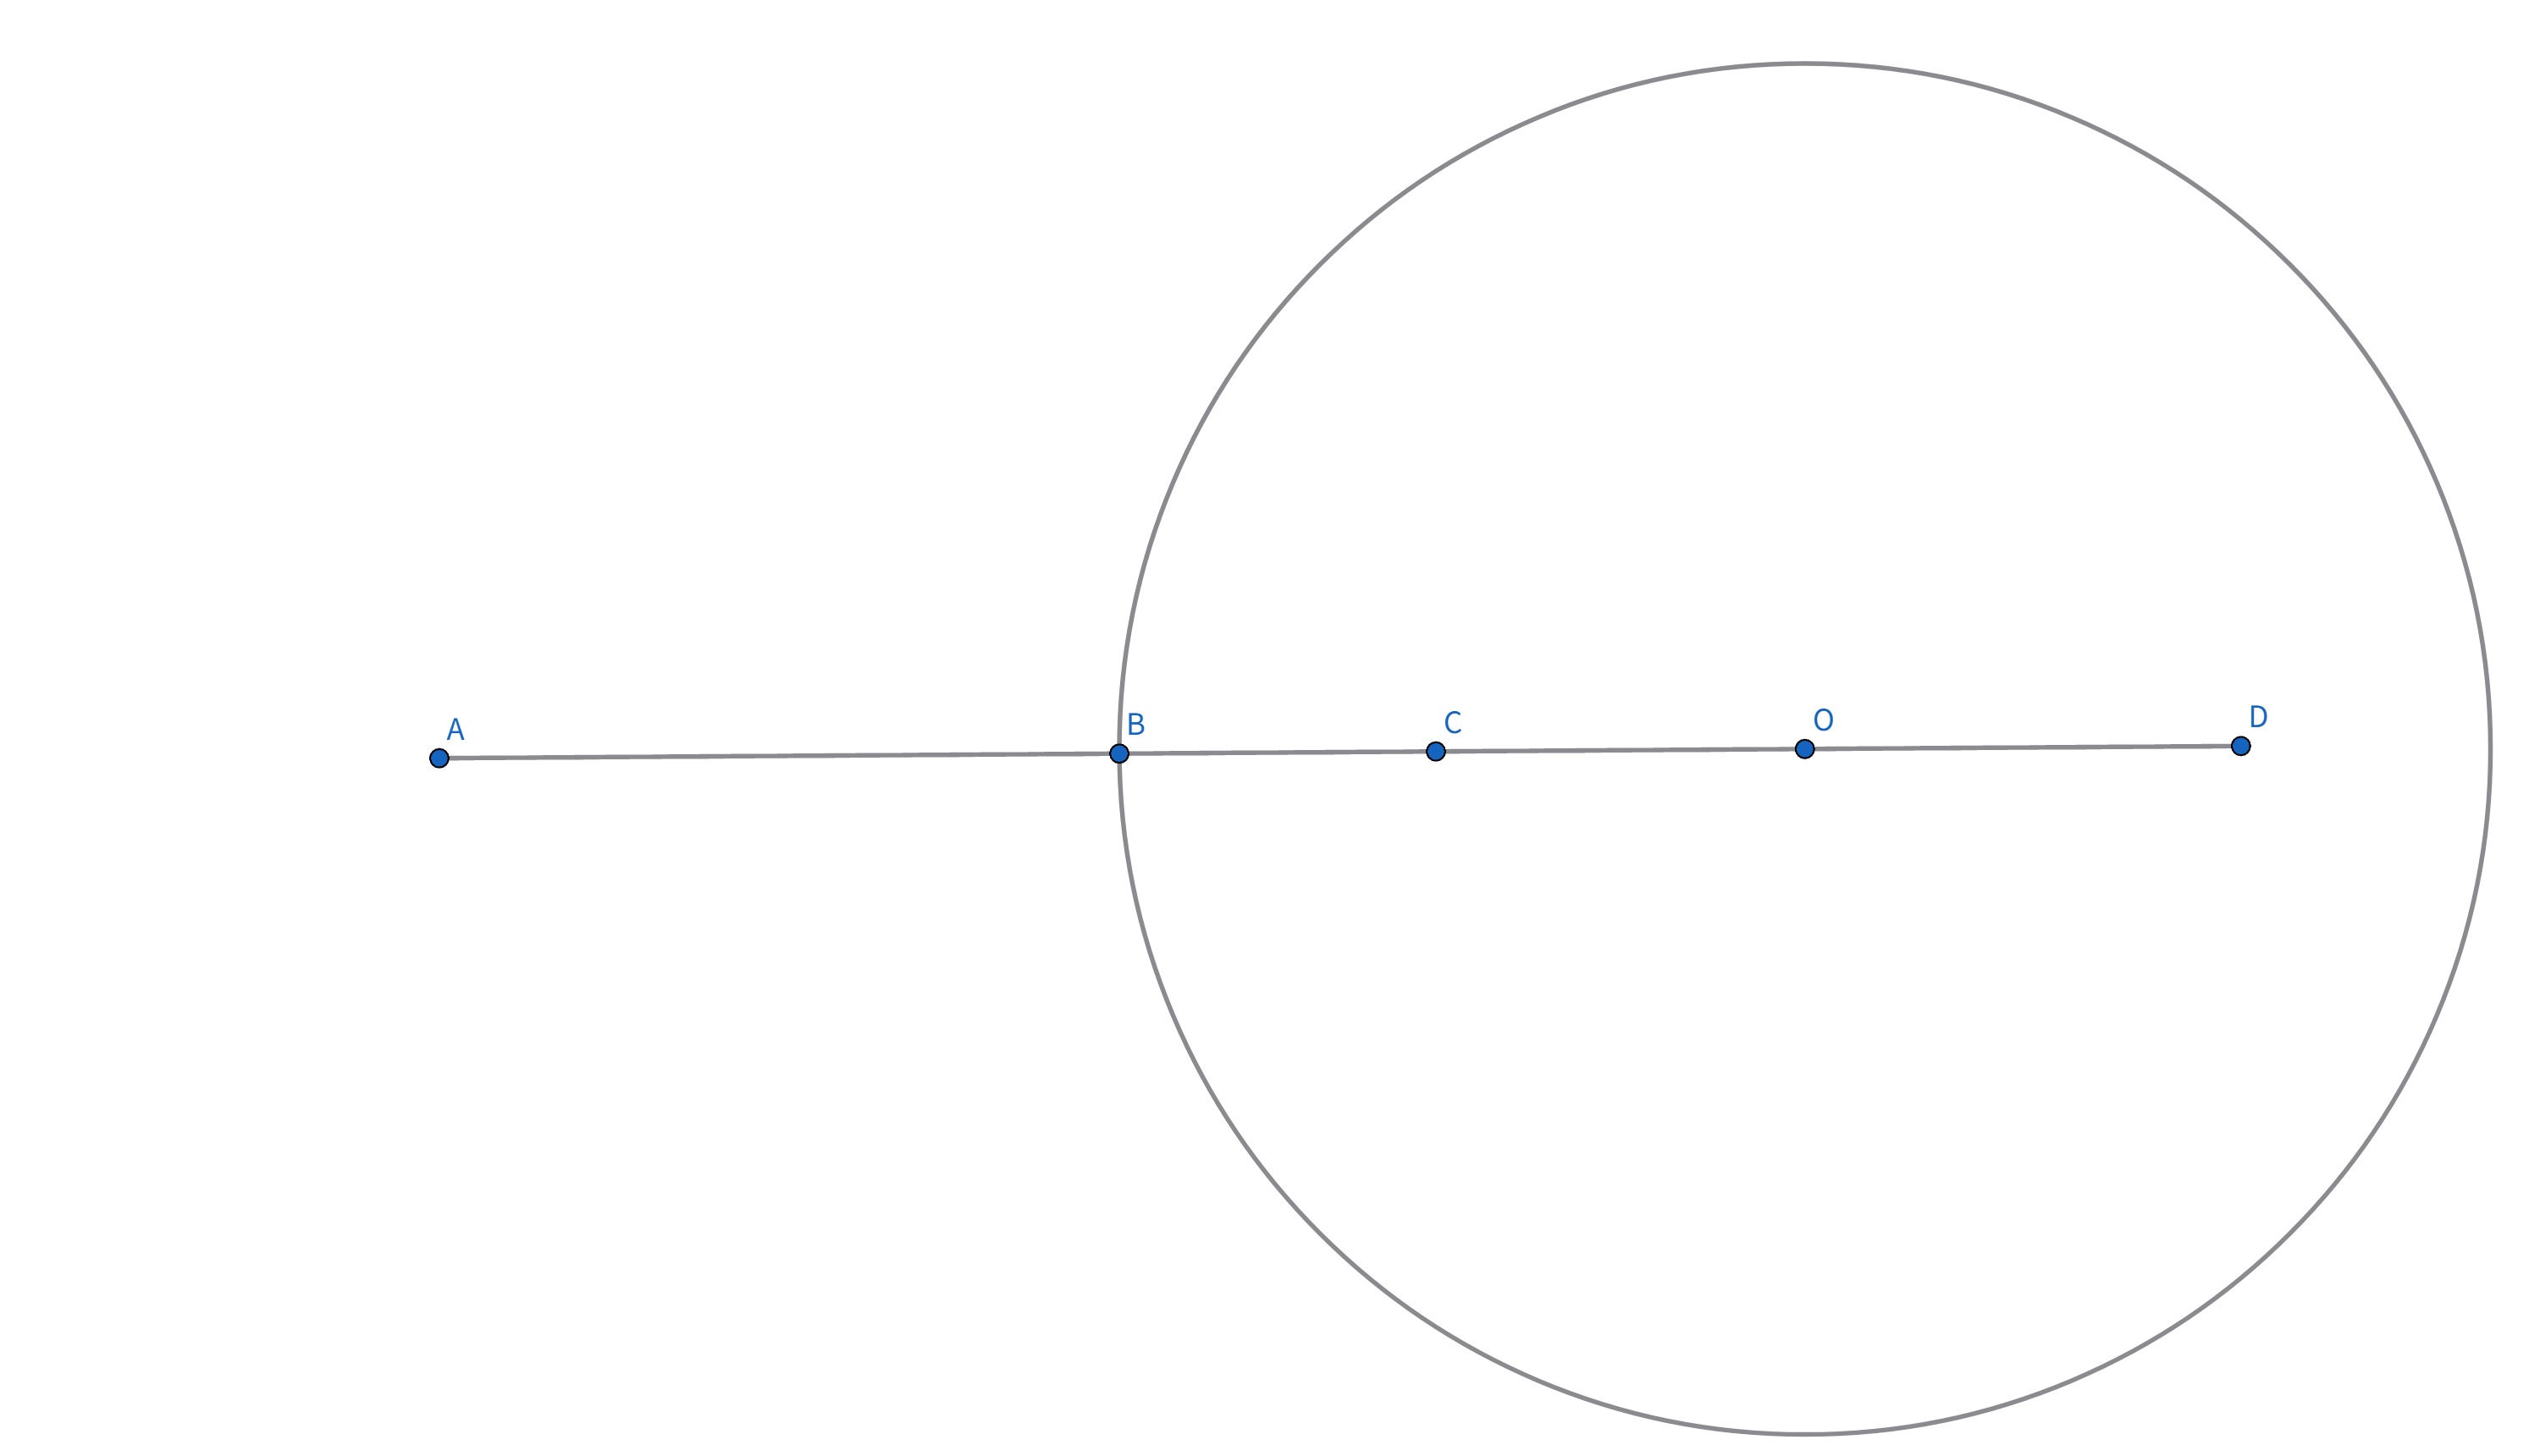
\includegraphics[width=0.8\linewidth]{figures/点与圆.png}
    % \caption{Caption}
    % \label{fig:enter-label}
\end{figure}

设XY为圆O的直径,$\angle XPY$也可以反应点P与圆O的关系。
\begin{itemize}
    \item 点在圆外:$\angle XAY< 90^\circ$。
    \item 点在圆上:$\angle XBY= 90^\circ$。
    \item 点在圆内:$\angle XCY > 90^\circ$。
\end{itemize}
\begin{figure}[H]
    \centering
    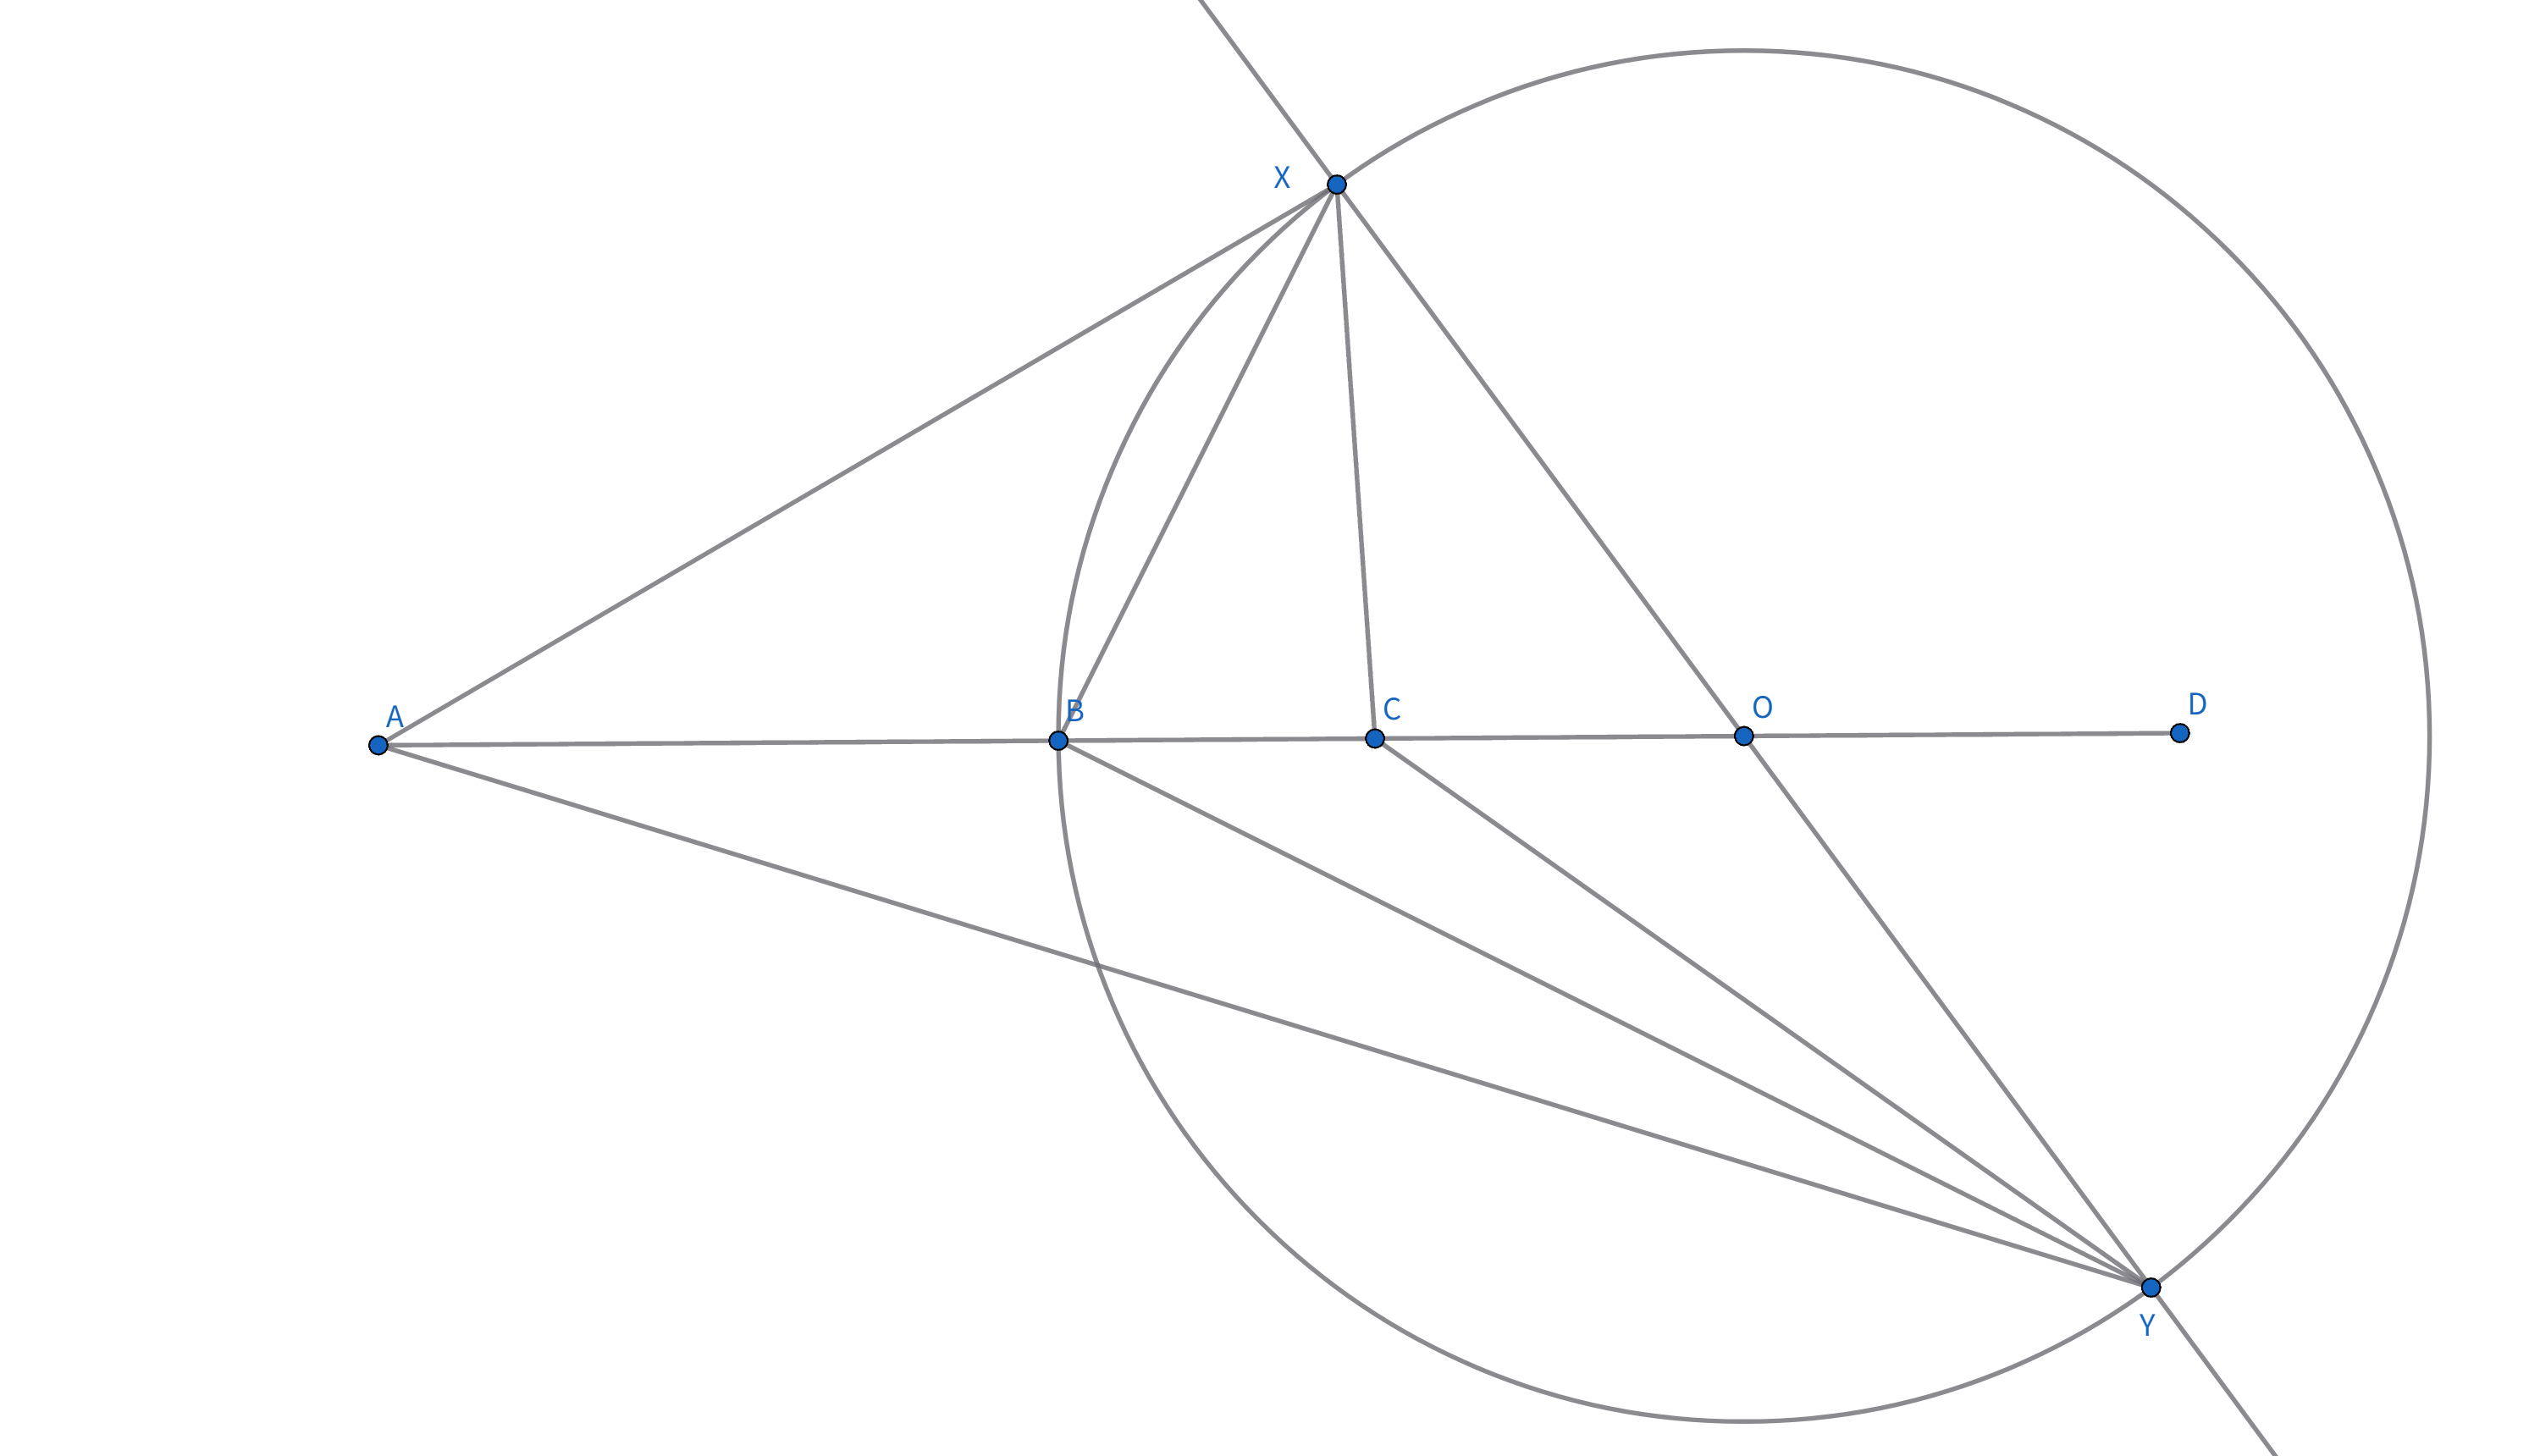
\includegraphics[width=0.8\linewidth]{figures/点与圆2.png}
    % \caption{Caption}
    % \label{fig:enter-label}
\end{figure}

\begin{example}
    对任意凸四边形ABCD以及形内一点P,以四边为直径作圆,则P至少在一个圆的内部。
\end{example}


\newpage 
\section{直线与圆的位置关系}
考虑直线l与圆O的交点个数,或圆心到直线的距离,可以将直线与圆的位置关系分为三类。
\begin{itemize}
    \item 相离:$d(O,l_1)=OA > r$, 直线与圆无交点。
    \item 相切:$d(O,l_1)=OA > r$, 直线与圆恰好有一个交点。称直线$l$ 为圆O的切线,交点称作切点。
    \item 相交:$d(O,l_1)=OA > r$, 直线与圆有两个交点。称$l$ 为圆O的割线,交点AB的连线段为圆O的弦。
\end{itemize}
\begin{figure}[H]
    \centering
    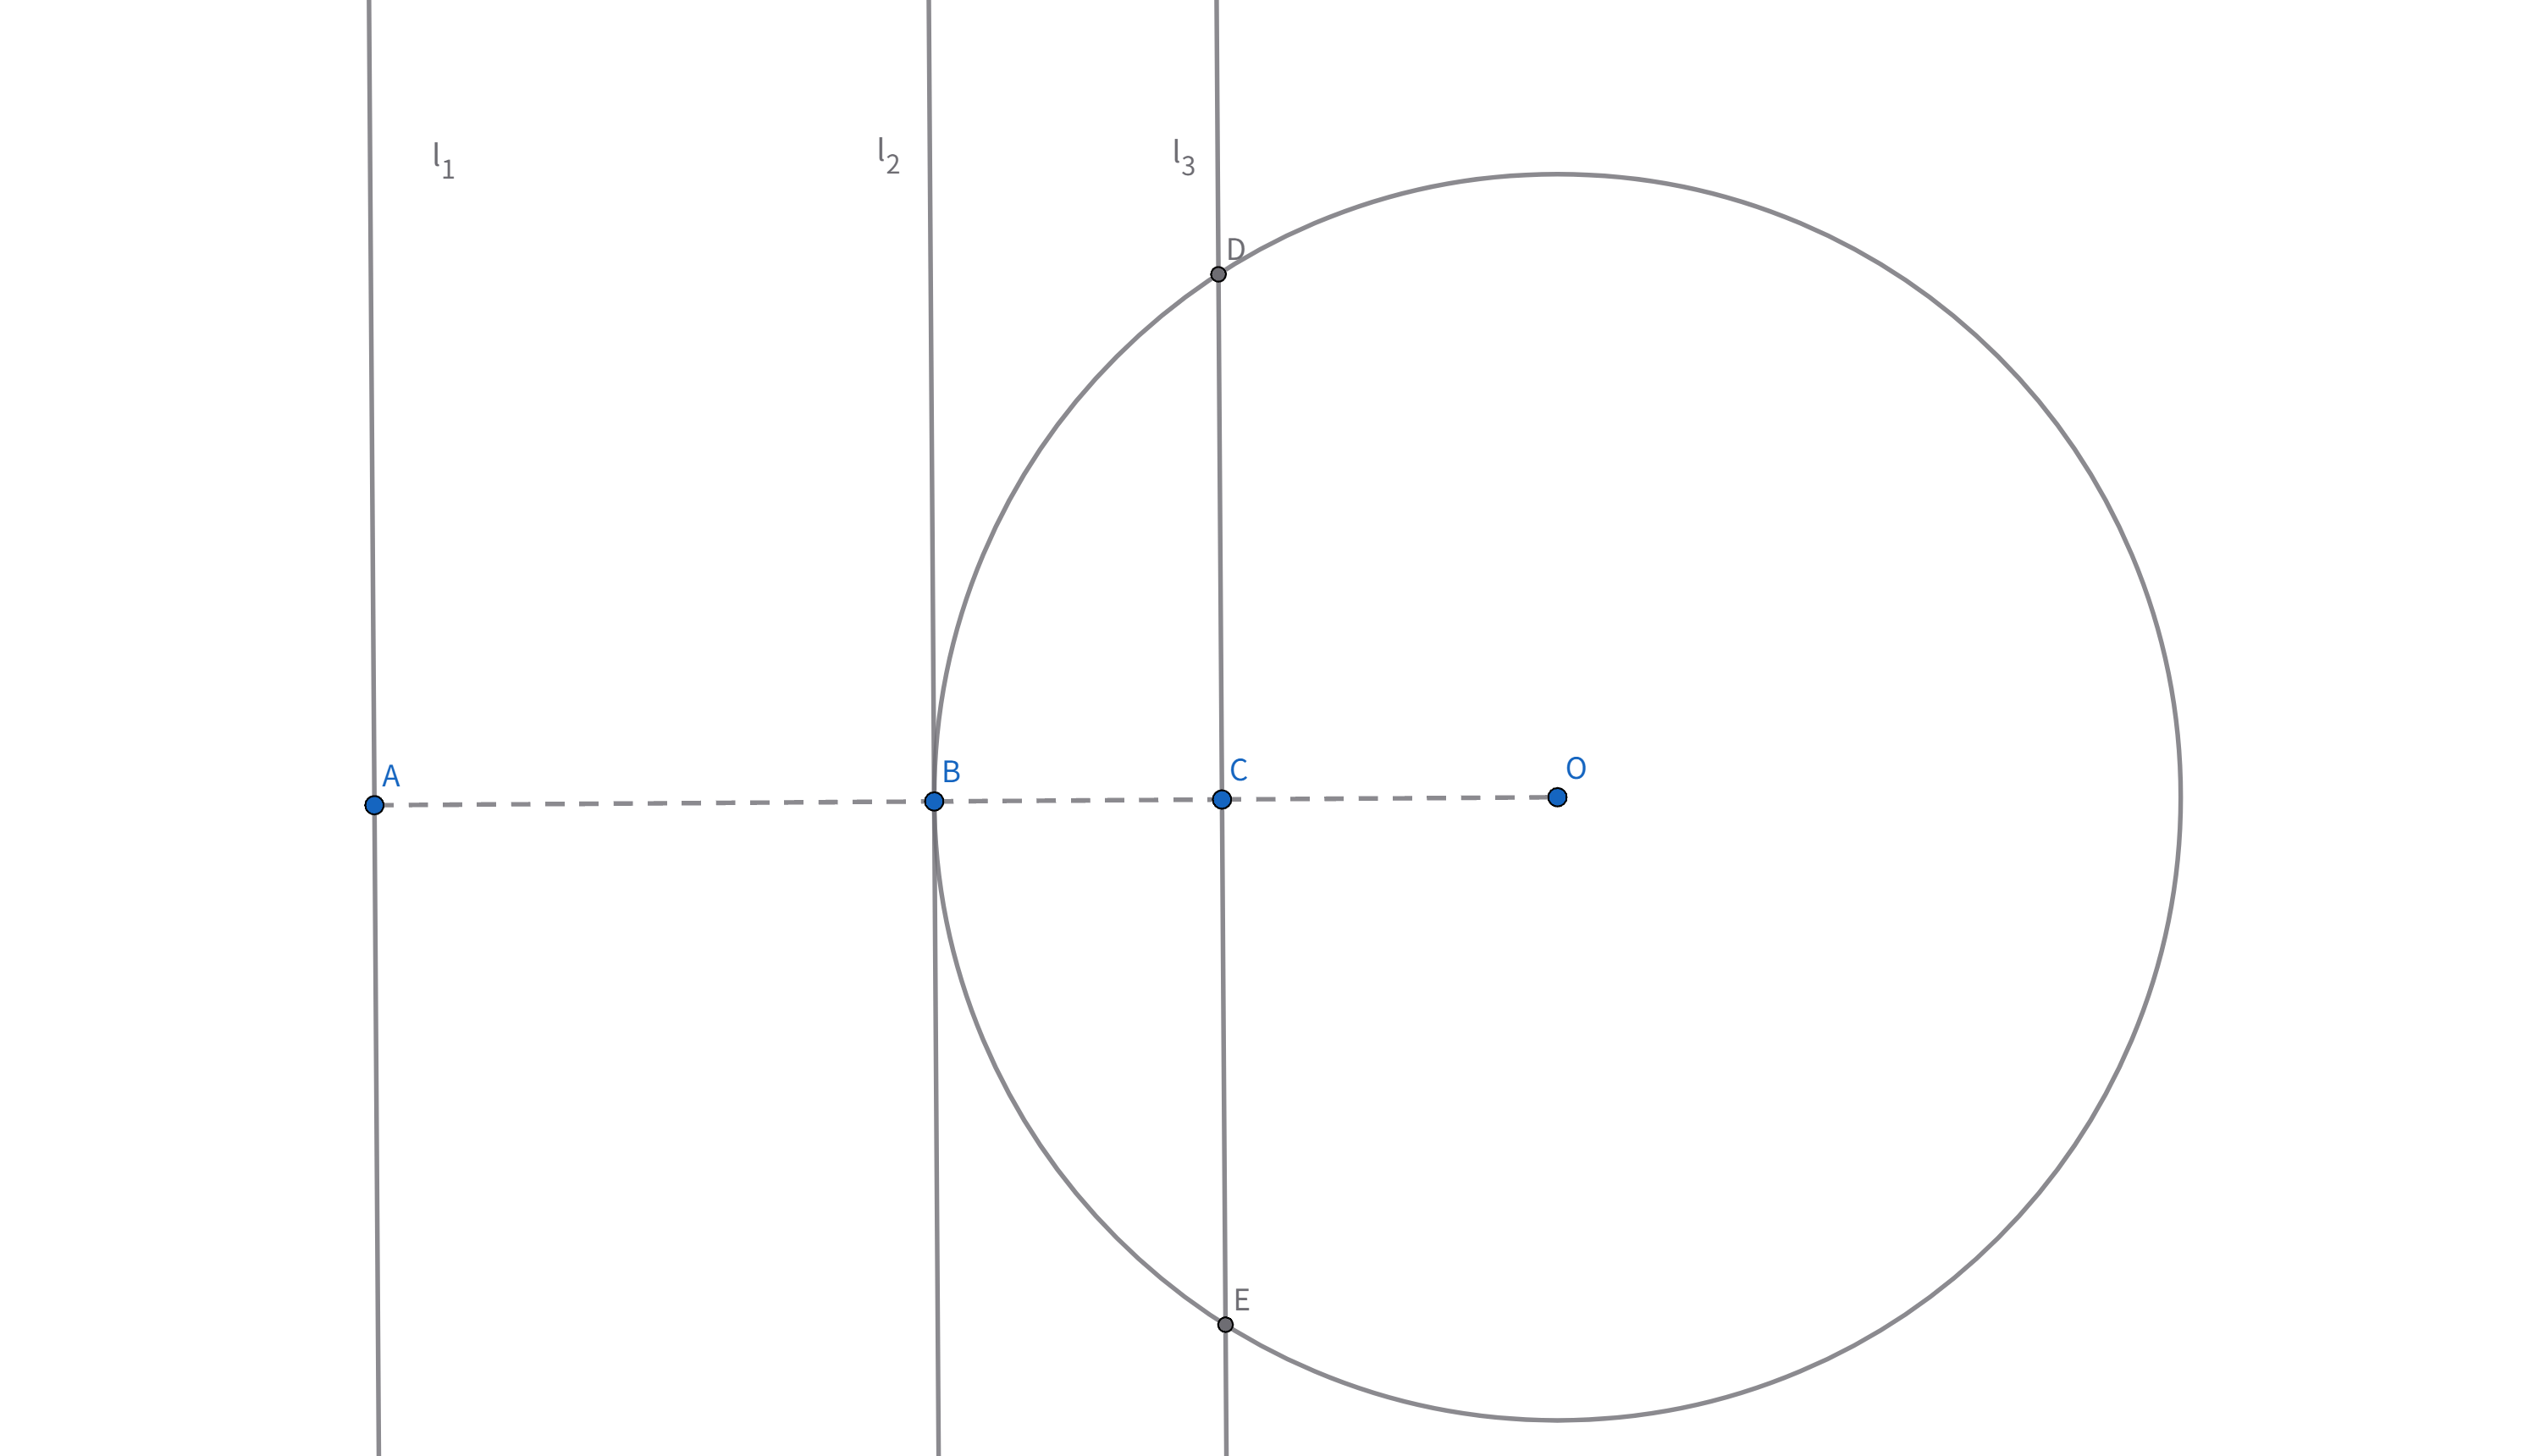
\includegraphics[width=0.8\linewidth]{figures/直线与圆.png}
    % \caption{Caption}
    % \label{fig:enter-label}
\end{figure}




\subsection{相交弦定理}
\begin{theorem}[相交弦定理]
    假设平面内有一半径为R的圆O,E为圆内一定点。过E作任意弦AC、BD,一定有
    $$
    AE \cdot EC =BE \cdot ED = R^2 - EO^2
    $$
\end{theorem}
\begin{figure}[H]
    \centering
    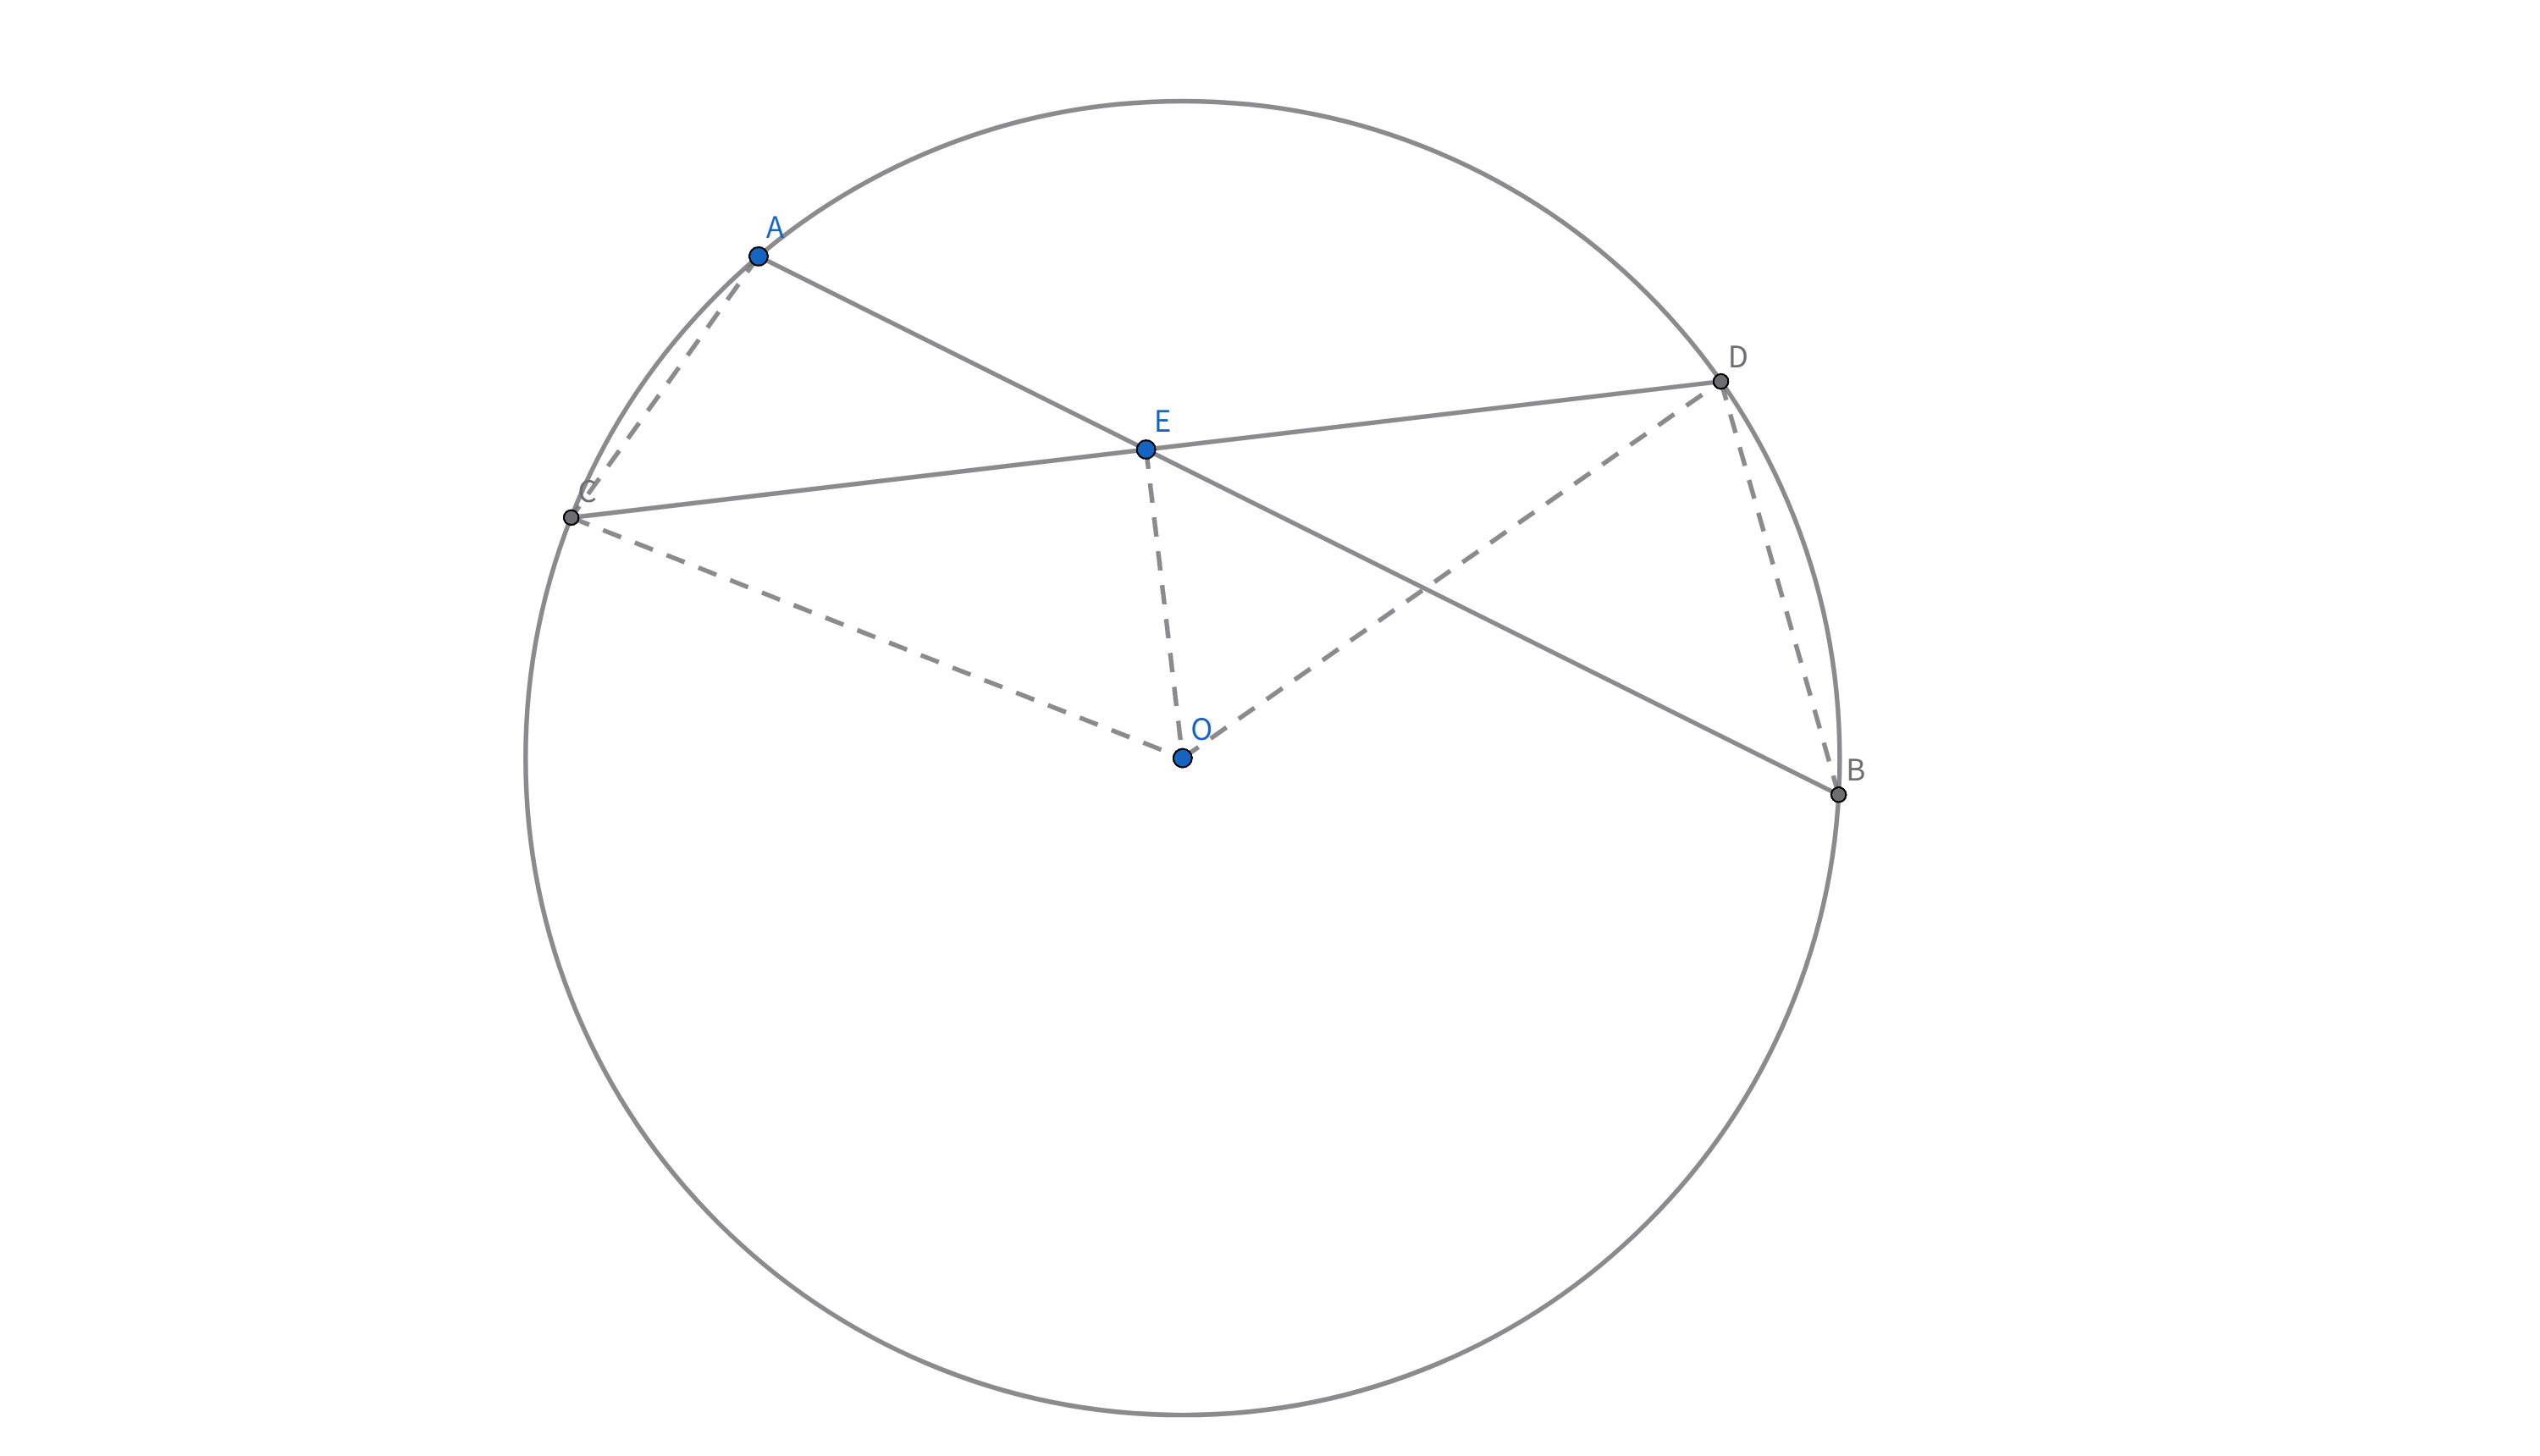
\includegraphics[width=0.7\linewidth]{figures/相交弦定理.png}
    \caption{相交弦定理}
    % \label{fig:enter-label}
\end{figure}


% 割线定理
\subsection{割线定理}
\begin{theorem}[割线定理]
   假设平面内有一半径为R的圆O,E为圆外一定点。过E作两条圆O割线分别交于AB、CD,一定有
$$
EA \cdot EB =EC \cdot ED = EO^2 -R^2
$$
\end{theorem}
\begin{figure}[H]
    \centering
    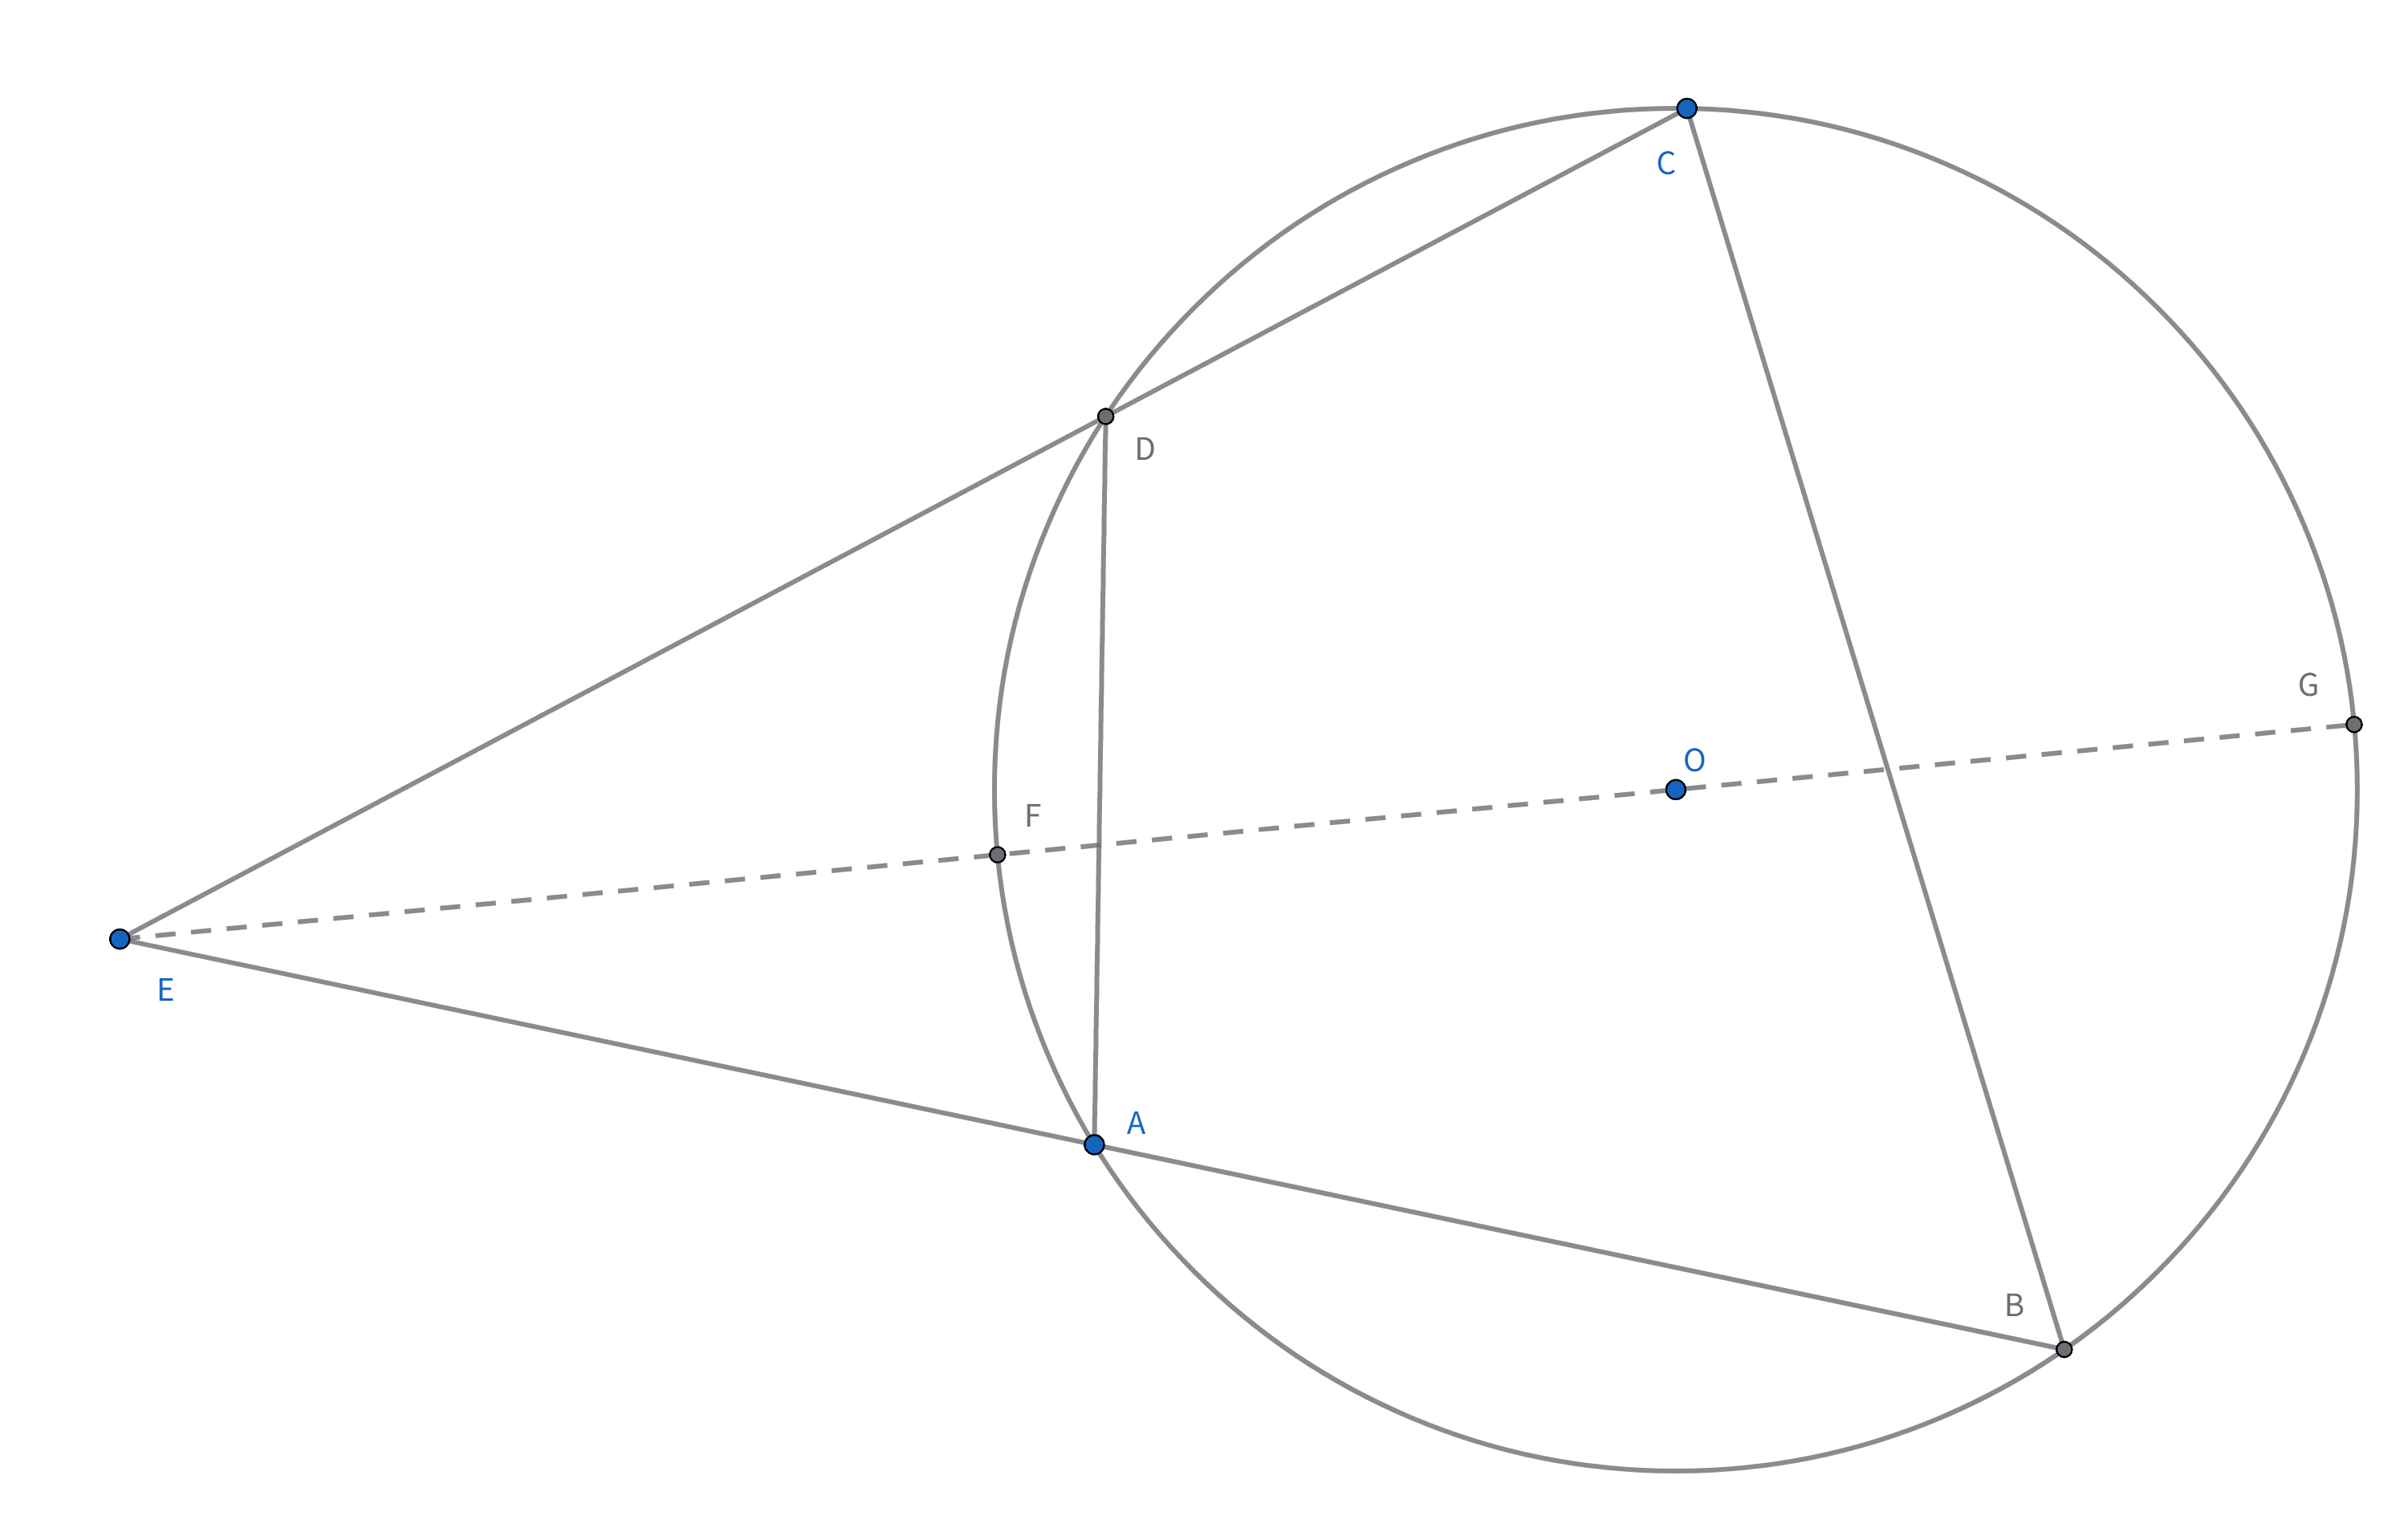
\includegraphics[width=0.7\linewidth]{figures/割线定理.png}
    \caption{割线定理}
    % \label{fig:enter-label}
\end{figure}


% 切割线定理]
\subsection{切割线定理}

\begin{proposition}[切线准则]
假设$\triangle ABC$的外心为$O$,$E$是平面上一点,则下面的条件等价:

(1) $PA$与圆$(ABC)$相切。

(2) $OA \perp AP.$

(3) $\angle PBA = \angle PCB.$
\end{proposition}
\proposition{切线准则}

\begin{theorem}[切割线定理]
    假设平面内有一半径为R的圆O,E为圆外一定点。过E作任意割线交圆于AC,作切线交圆于B,一定有
    $$
    EB^2 = EA \cdot EC = EO^2 - R^2
    $$
\end{theorem}
\begin{figure}[H]
    \centering
    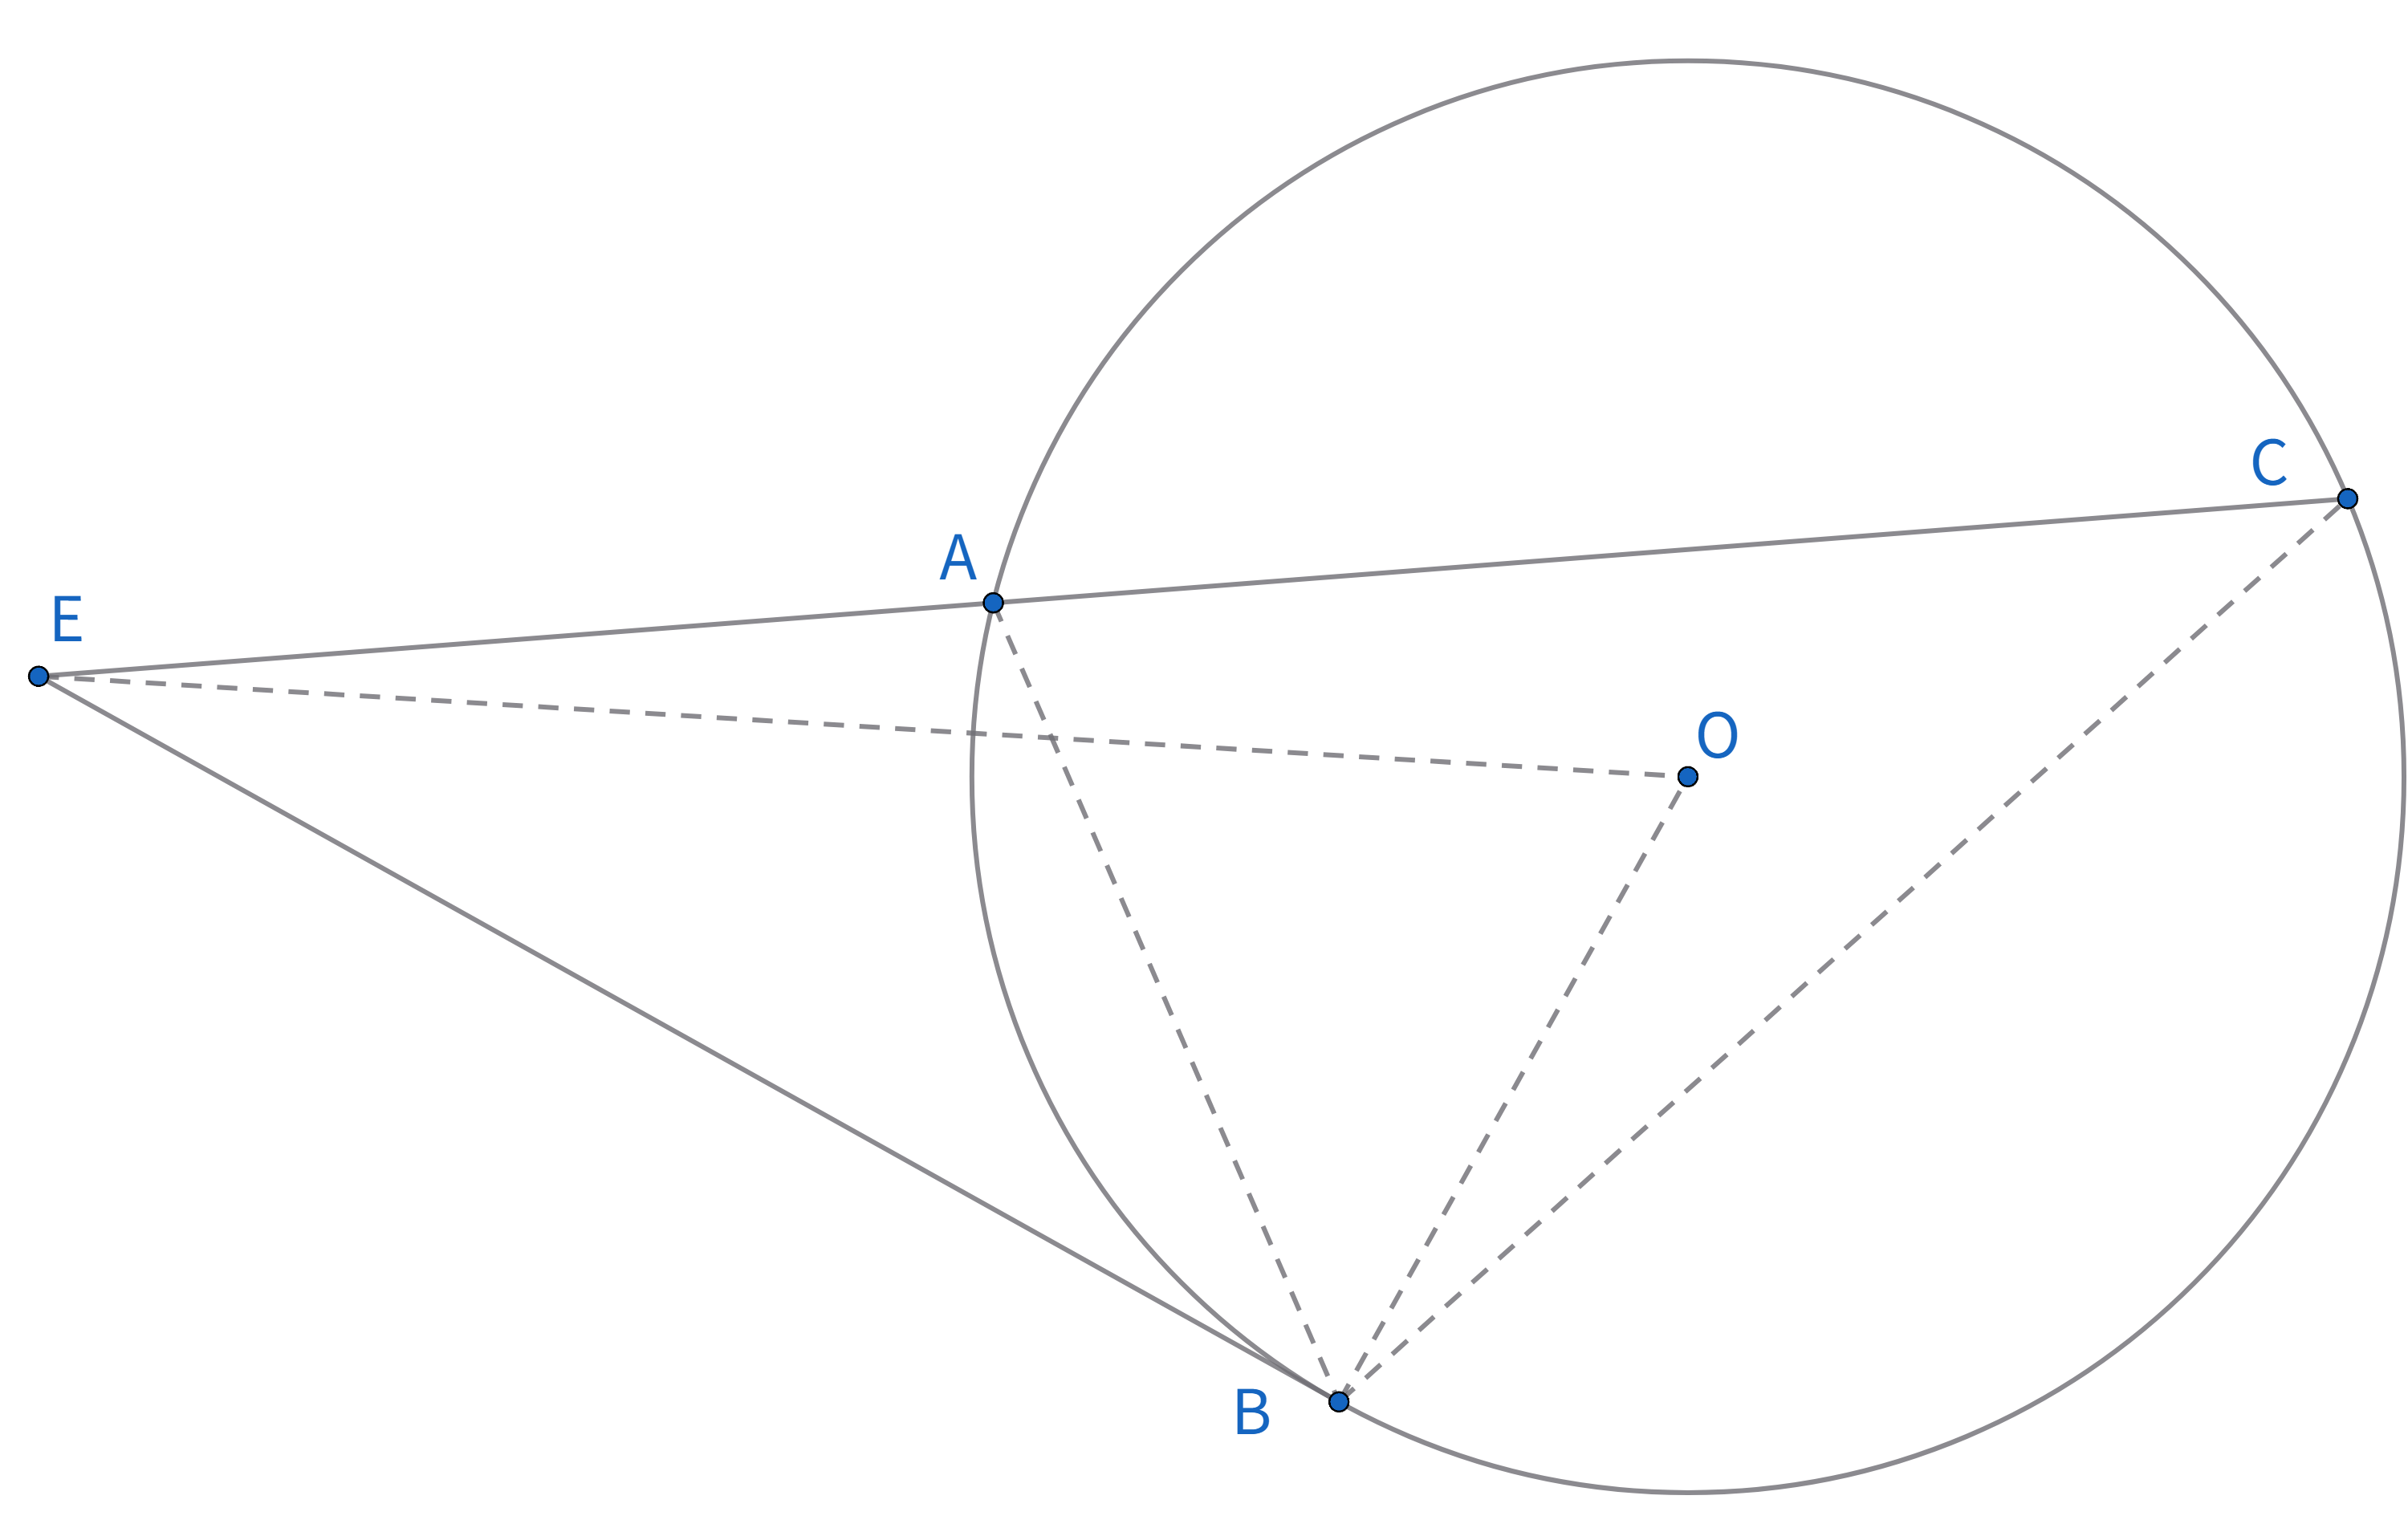
\includegraphics[width=0.7\linewidth]{figures/切割弦定理.png}
    \caption{切割线定理}
\end{figure}


\subsection{圆与圆的位置关系}
圆与圆的位置关系可分为五类,包括外离、外切、相交、内切、内含。
\begin{itemize}
    \item 相离:两圆无交点,可分为外离与内含。
    \item 相切:两圆恰好有一个交点,交点称作切点,可分为外切与内切。
    \item 相交:两圆有两个交点,交点AB构成的连线段称作两圆的相交弦。
\end{itemize}
\begin{figure}[H]
    \centering
    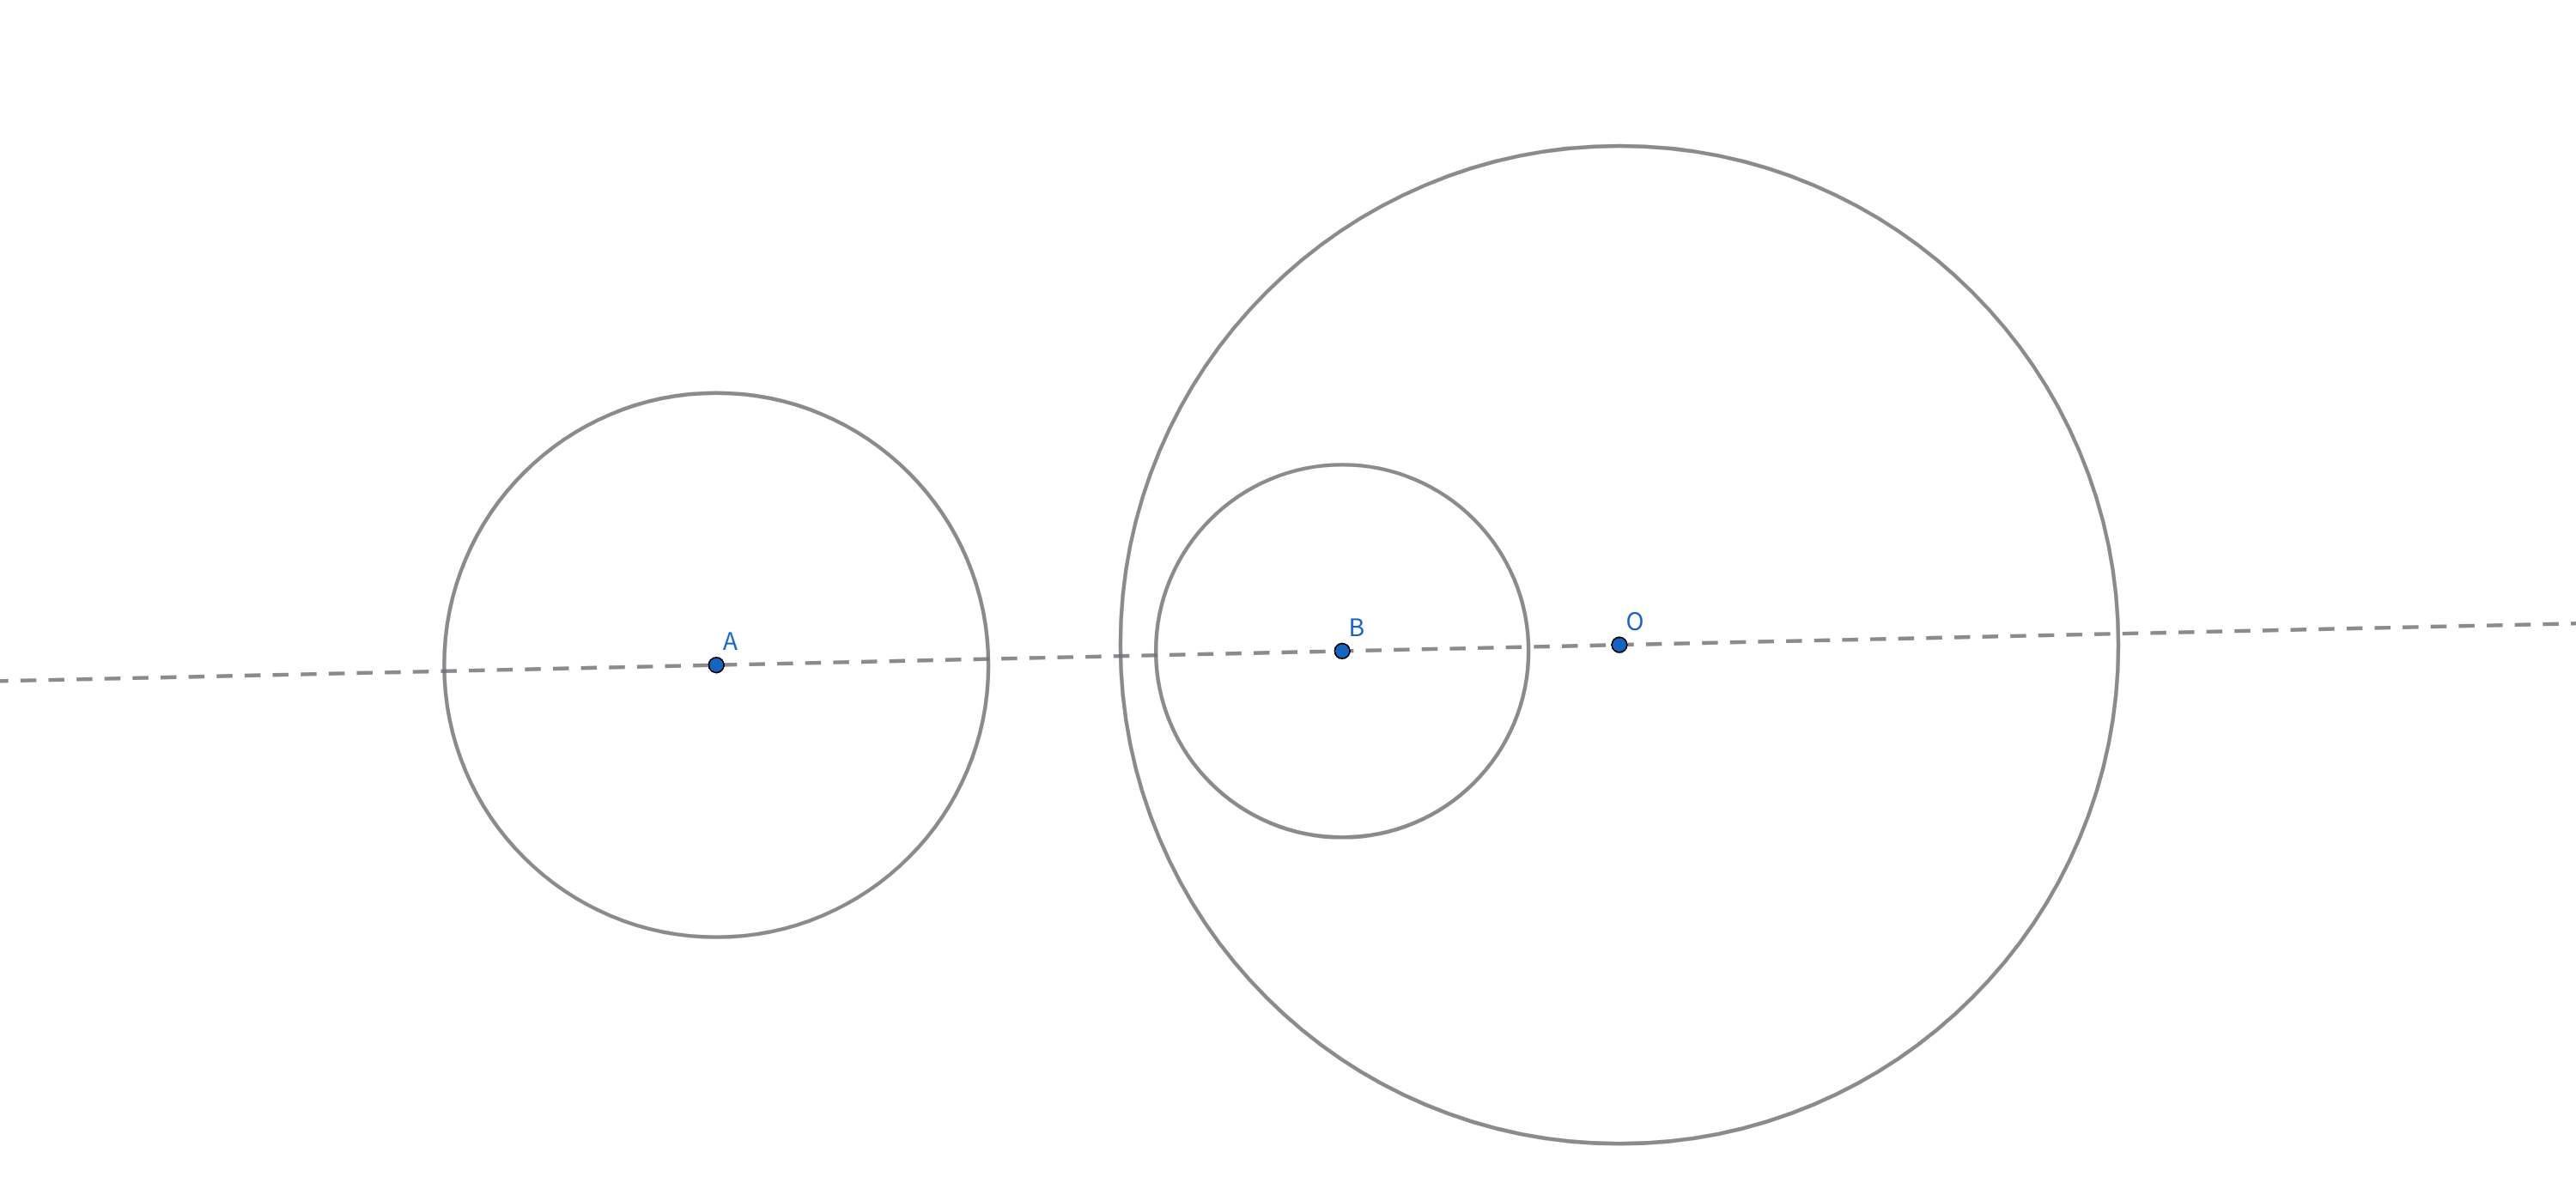
\includegraphics[width=0.5\linewidth]{figures/外离与内含.png}
    \caption{外离与内含}
    % \label{fig:enter-label}
\end{figure}
\begin{figure}[H]
    \centering
    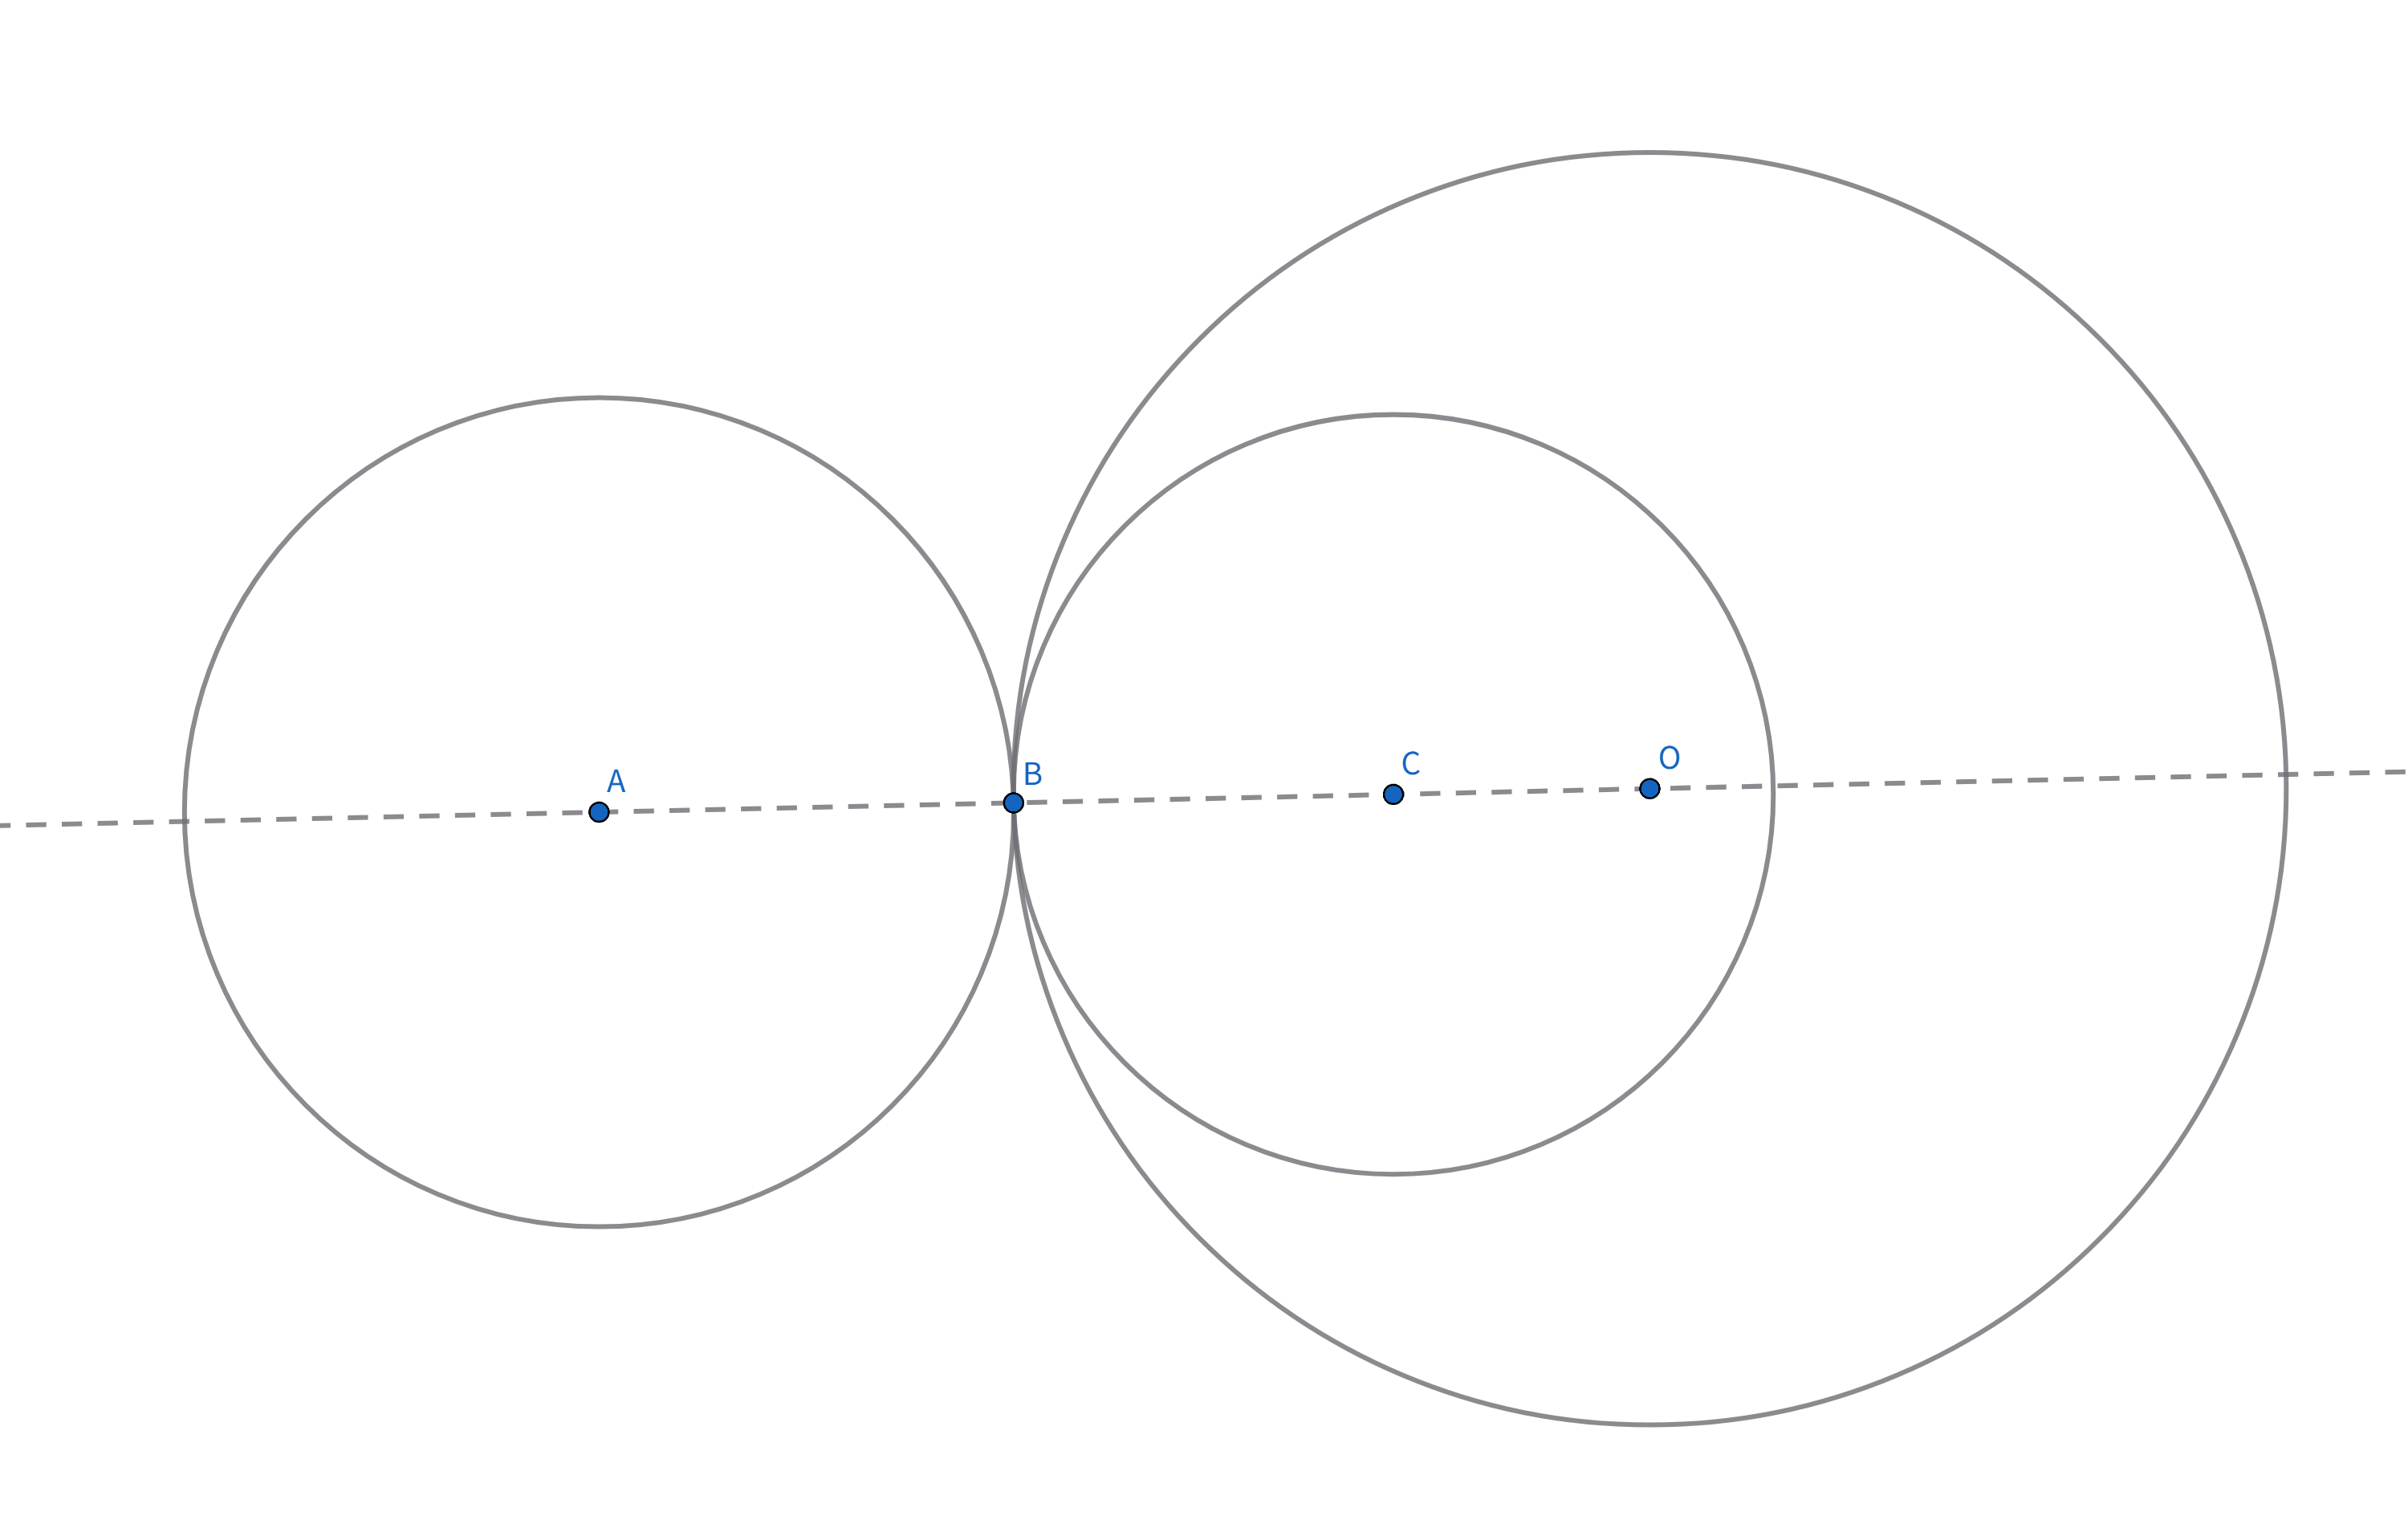
\includegraphics[width=0.5\linewidth]{figures/外切与内切.png}
    \caption{外切与内切}
    % \label{fig:enter-label}
\end{figure}
\begin{figure}[H]
    \centering
    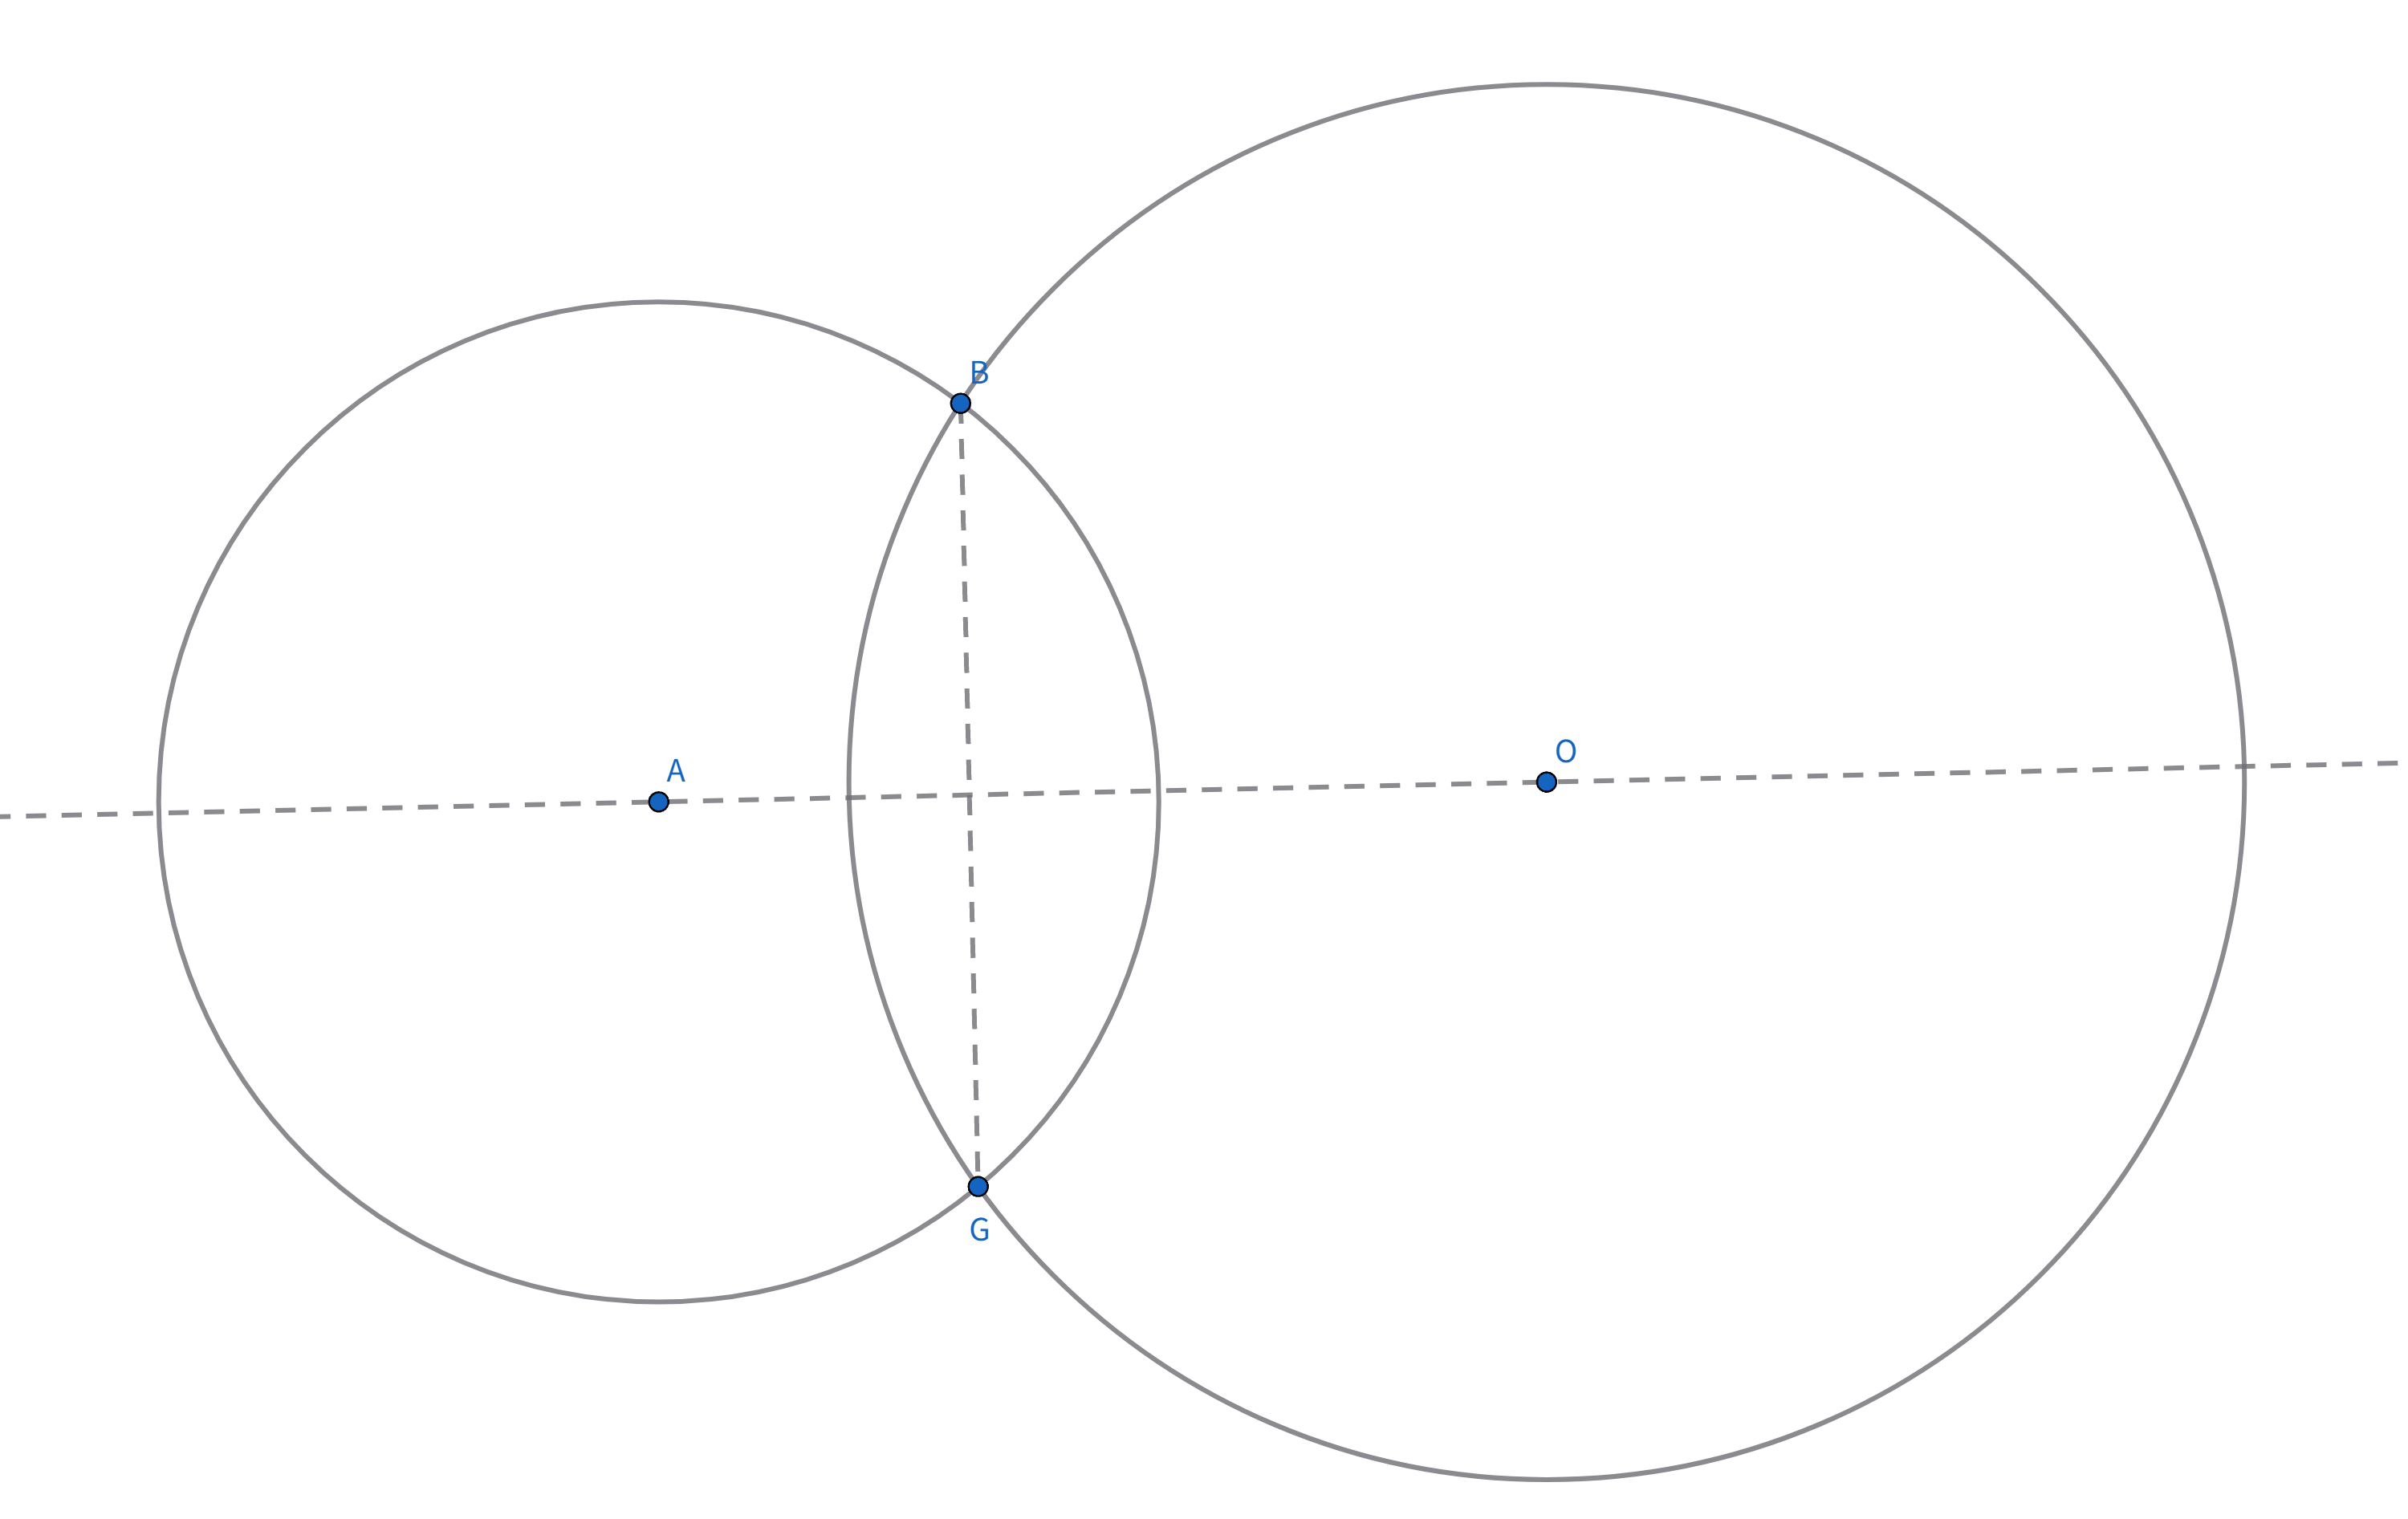
\includegraphics[width=0.5\linewidth]{figures/圆相交.png}
    \caption{圆相交}
    % \label{fig:enter-label}
\end{figure}


\newpage 
\section{外接圆}
\begin{definition}
任意不共线的三点A、B、C可以唯一确定一个圆,这个圆O称作是$\triangle ABC$的外接圆。

取三边BC、AB、AC的中点D、E、F,假设BC中垂线与AC中垂线交于O,则A、B、C三点一定在以O为圆心,以OA为半径的圆上。    
\end{definition}

\begin{theorem}
    对任意 $\triangle ABC$,一定有下式成立:
    $$\frac{BC}{\sin A} = \frac{AC}{\sin B} = \frac{AB}{\sin C}=2R.$$
\end{theorem}
\begin{figure}[H]
    \centering
    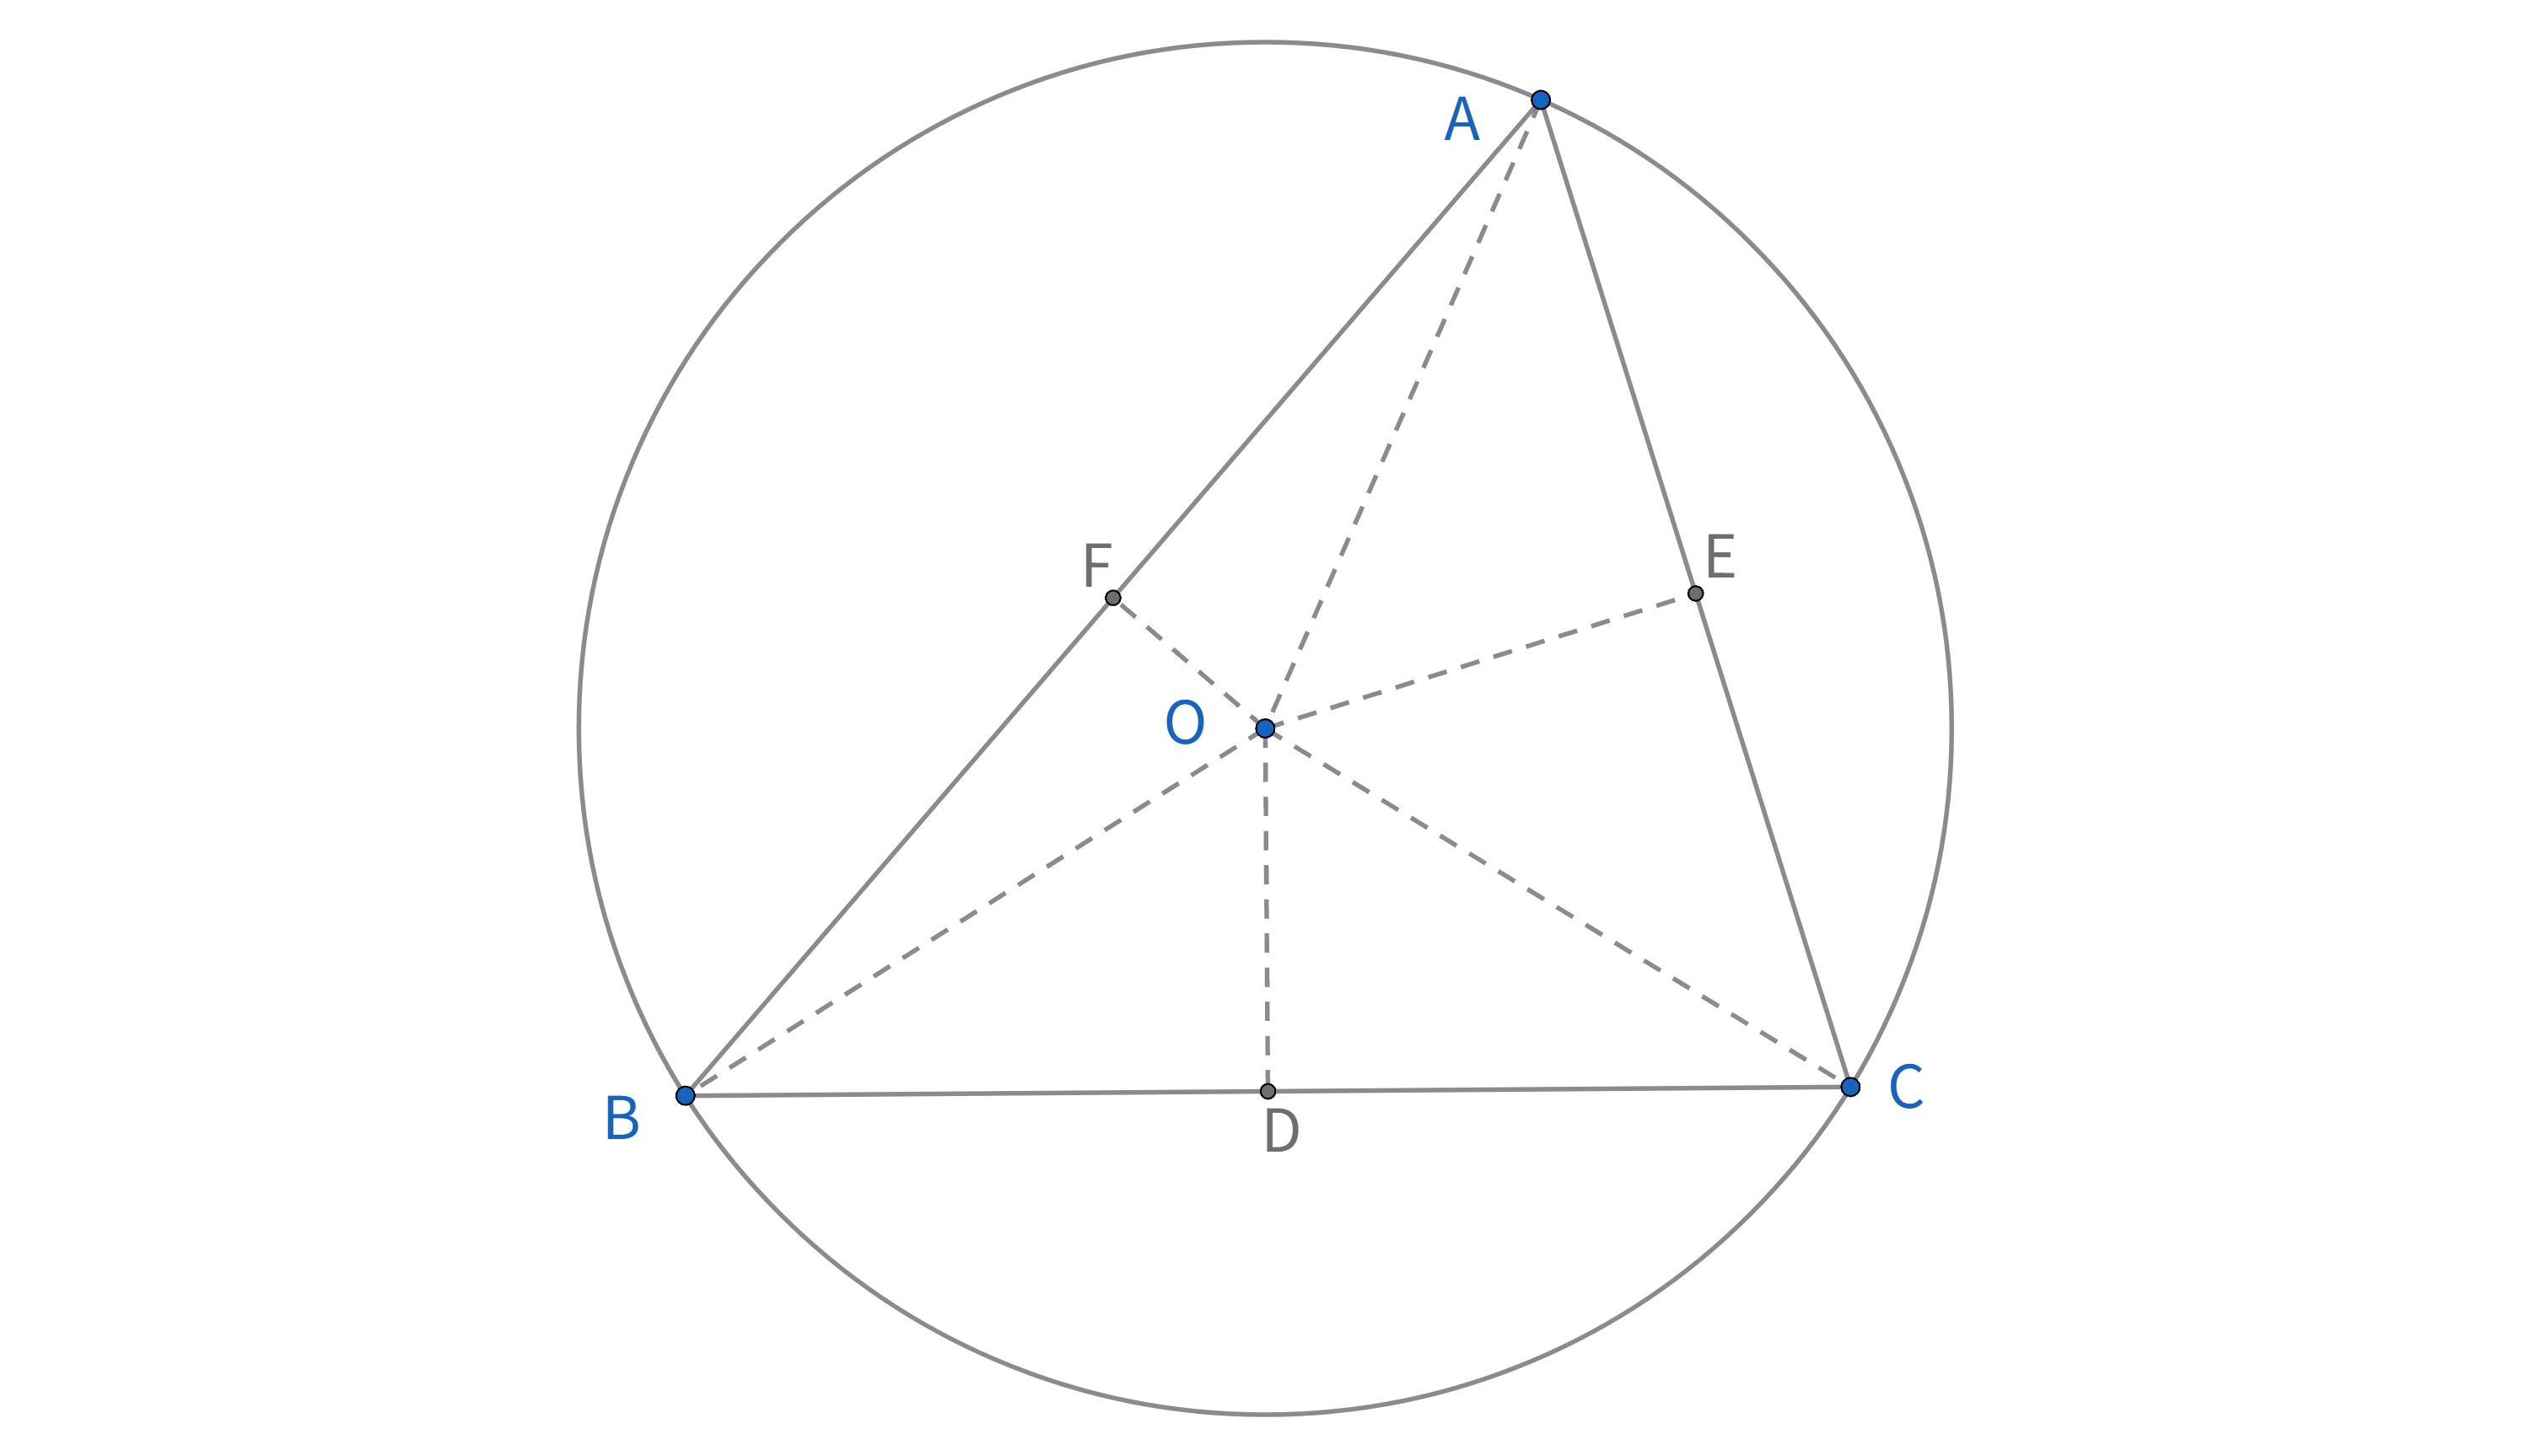
\includegraphics[width=\linewidth]{figures/正弦定理.png}
    \caption{正弦定理}
\end{figure}

\newpage 
\section{四点共圆}
\begin{proposition}[四点共圆判定方法]
    四边形ABCD顶点均在圆O上,等价于下列任一条件成立。

    (1) A、B、C、D到同一点O的距离相同。

    (2) 存在一组对角互补。

    (3) 有一边与另两点构成的顶角度数相同。

    (4) 对角线交于F点,$AF\cdot FC = BF\cdot FD$。

    (5) 有一组对边AB、CD的延长线相交于E,若$EA\cdot EB = ED\cdot EC$。
\end{proposition}
\begin{figure}[H]
    \centering
    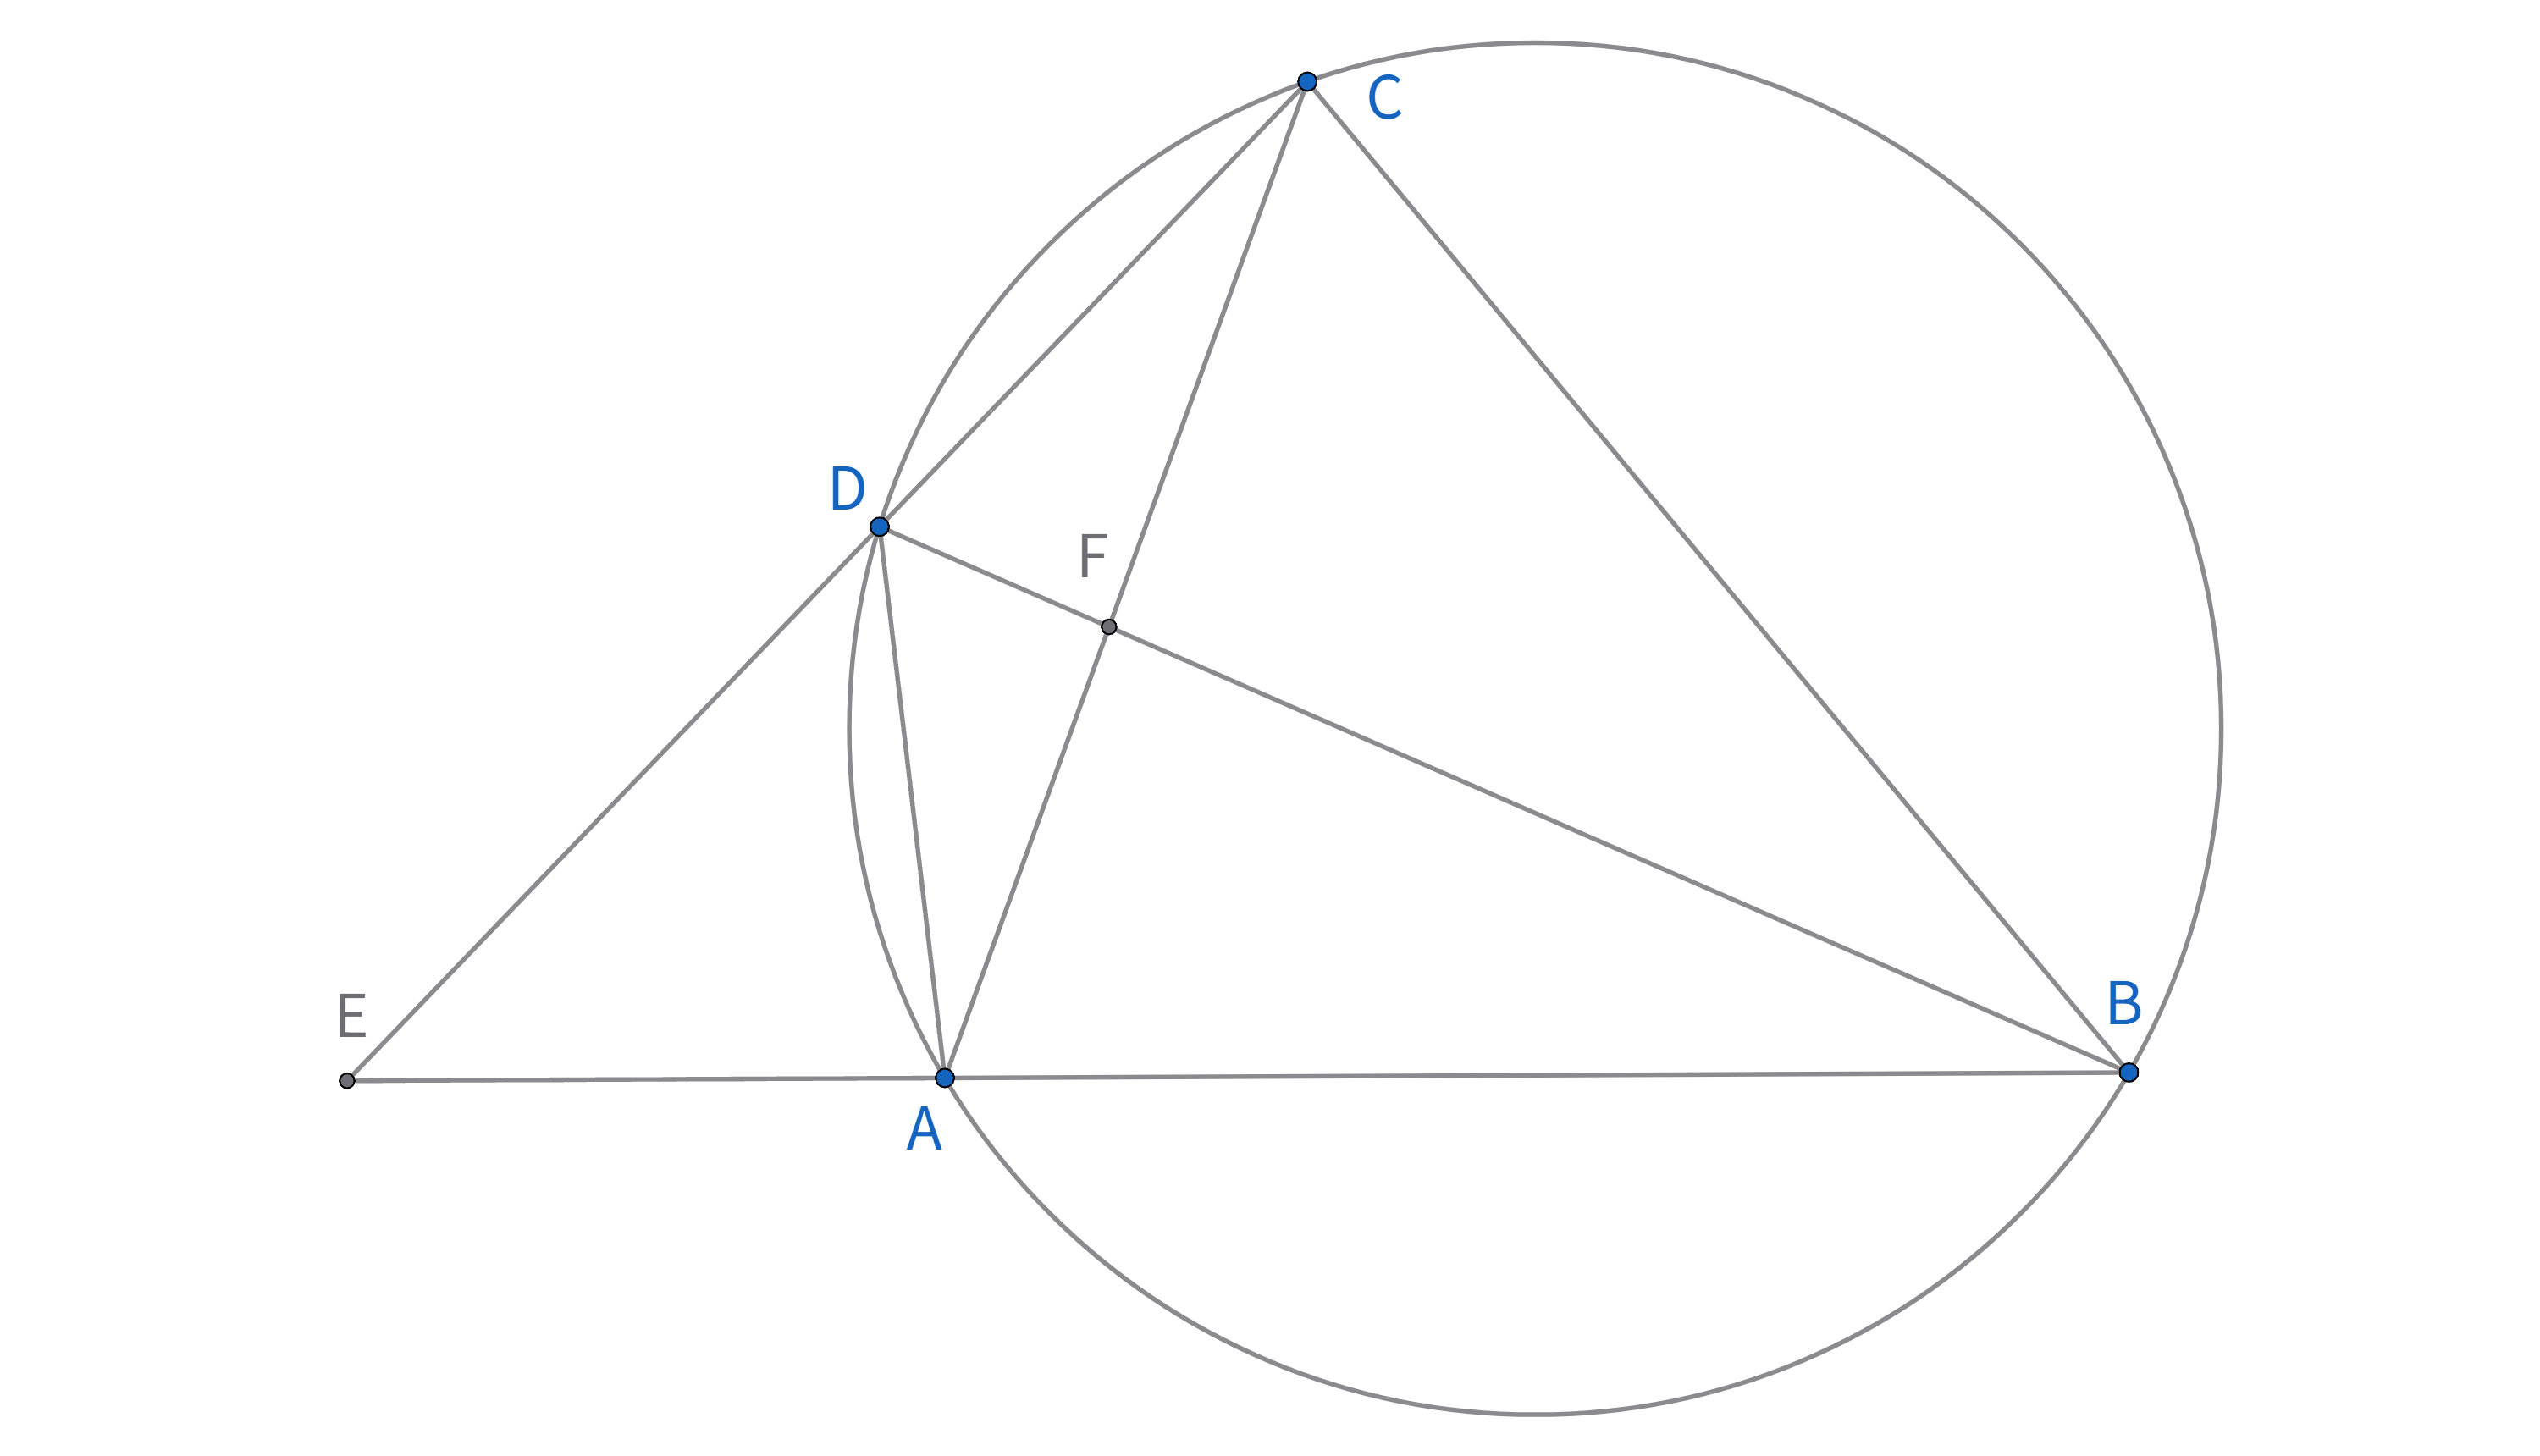
\includegraphics[width=\linewidth]{figures/四点共圆.png}
    % \caption{Caption}
    % \label{fig:enter-label}
\end{figure}


\begin{exercise}
梯形是圆内接四边形当且仅当它是等腰梯形。
\end{exercise}


\begin{exercise}
在四边形 $WXYZ$ 中,对角线相互垂直,已知 $\angle WZX = 30^\circ$,$\angle XWY = 40^\circ$,$\angle WYZ = 50^\circ$。
(a) 求 $\angle WZY$;
(b) 求 $\angle WXY$。
\end{exercise}

\begin{figure}[H]
    \centering
    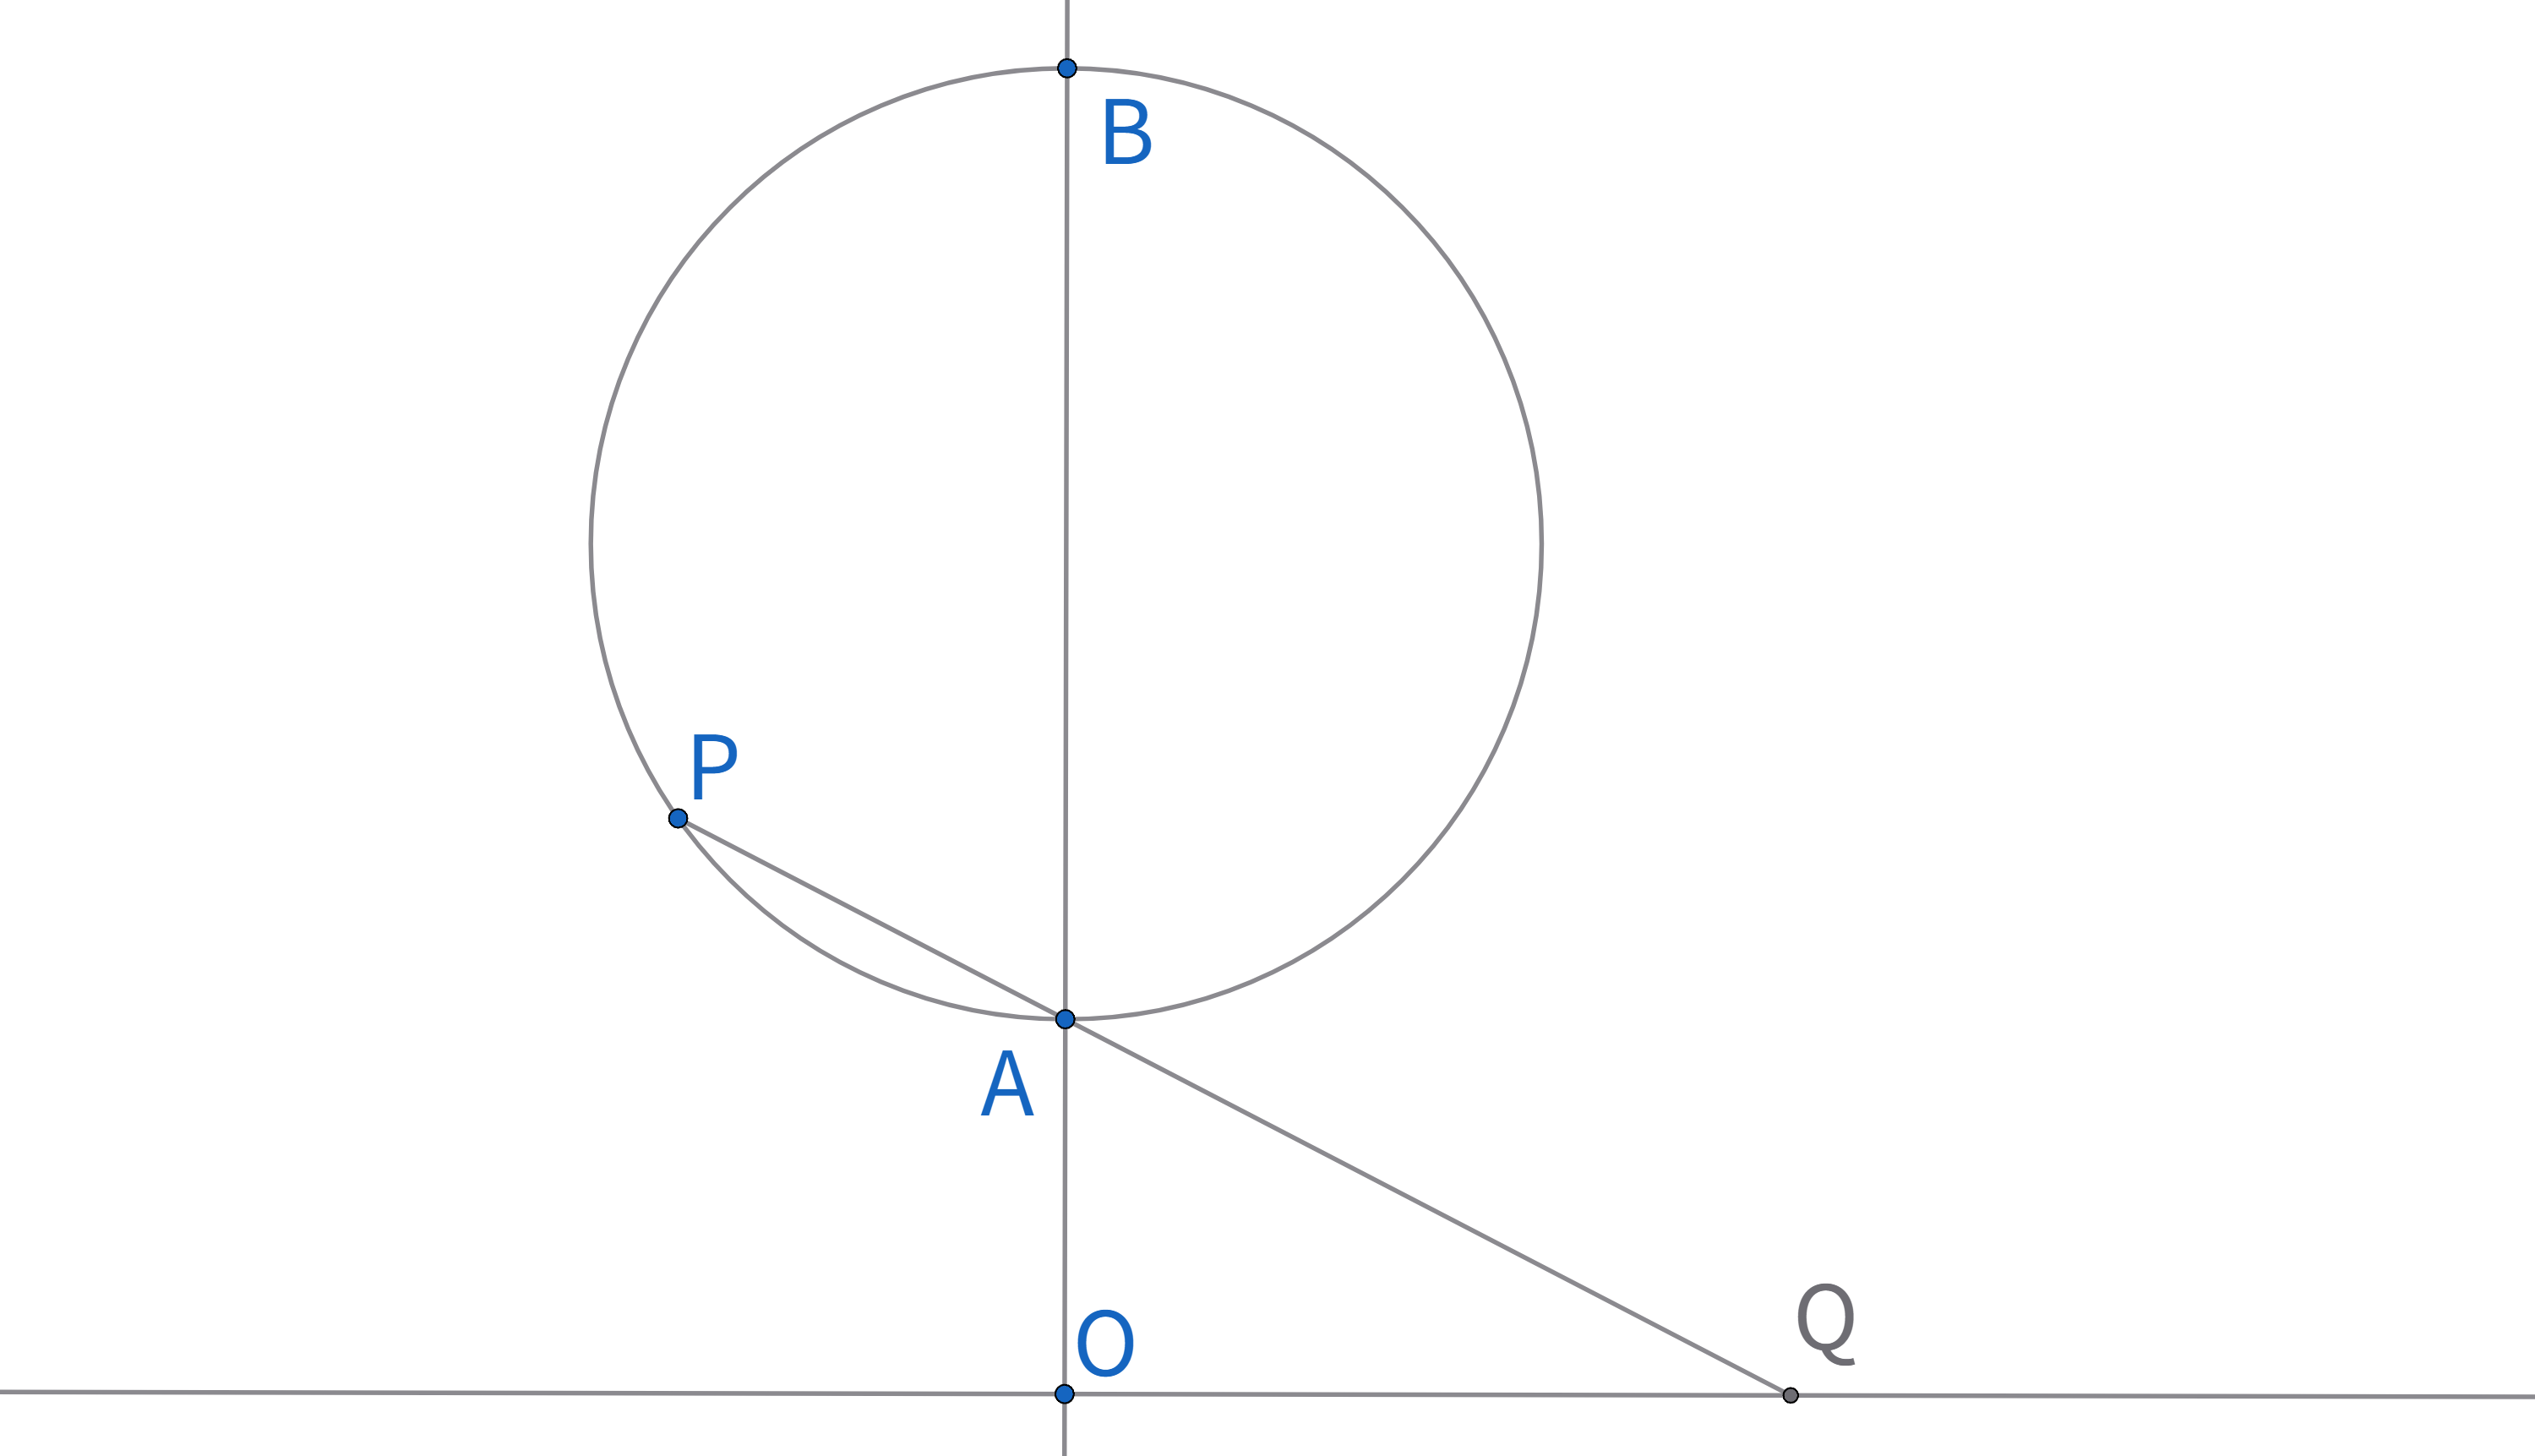
\includegraphics[width=0.7\linewidth]{figures/exercises/003.png}
\end{figure}

\begin{exercise}
设 $ABCDE$ 是一个凸五边形,其中 $BCDE$ 是正方形,中心为 $O$,$\angle A = 90^\circ$。证明:$AO$ 平分 $\angle BAE$。
\end{exercise}

\begin{figure}[H]
    \centering
    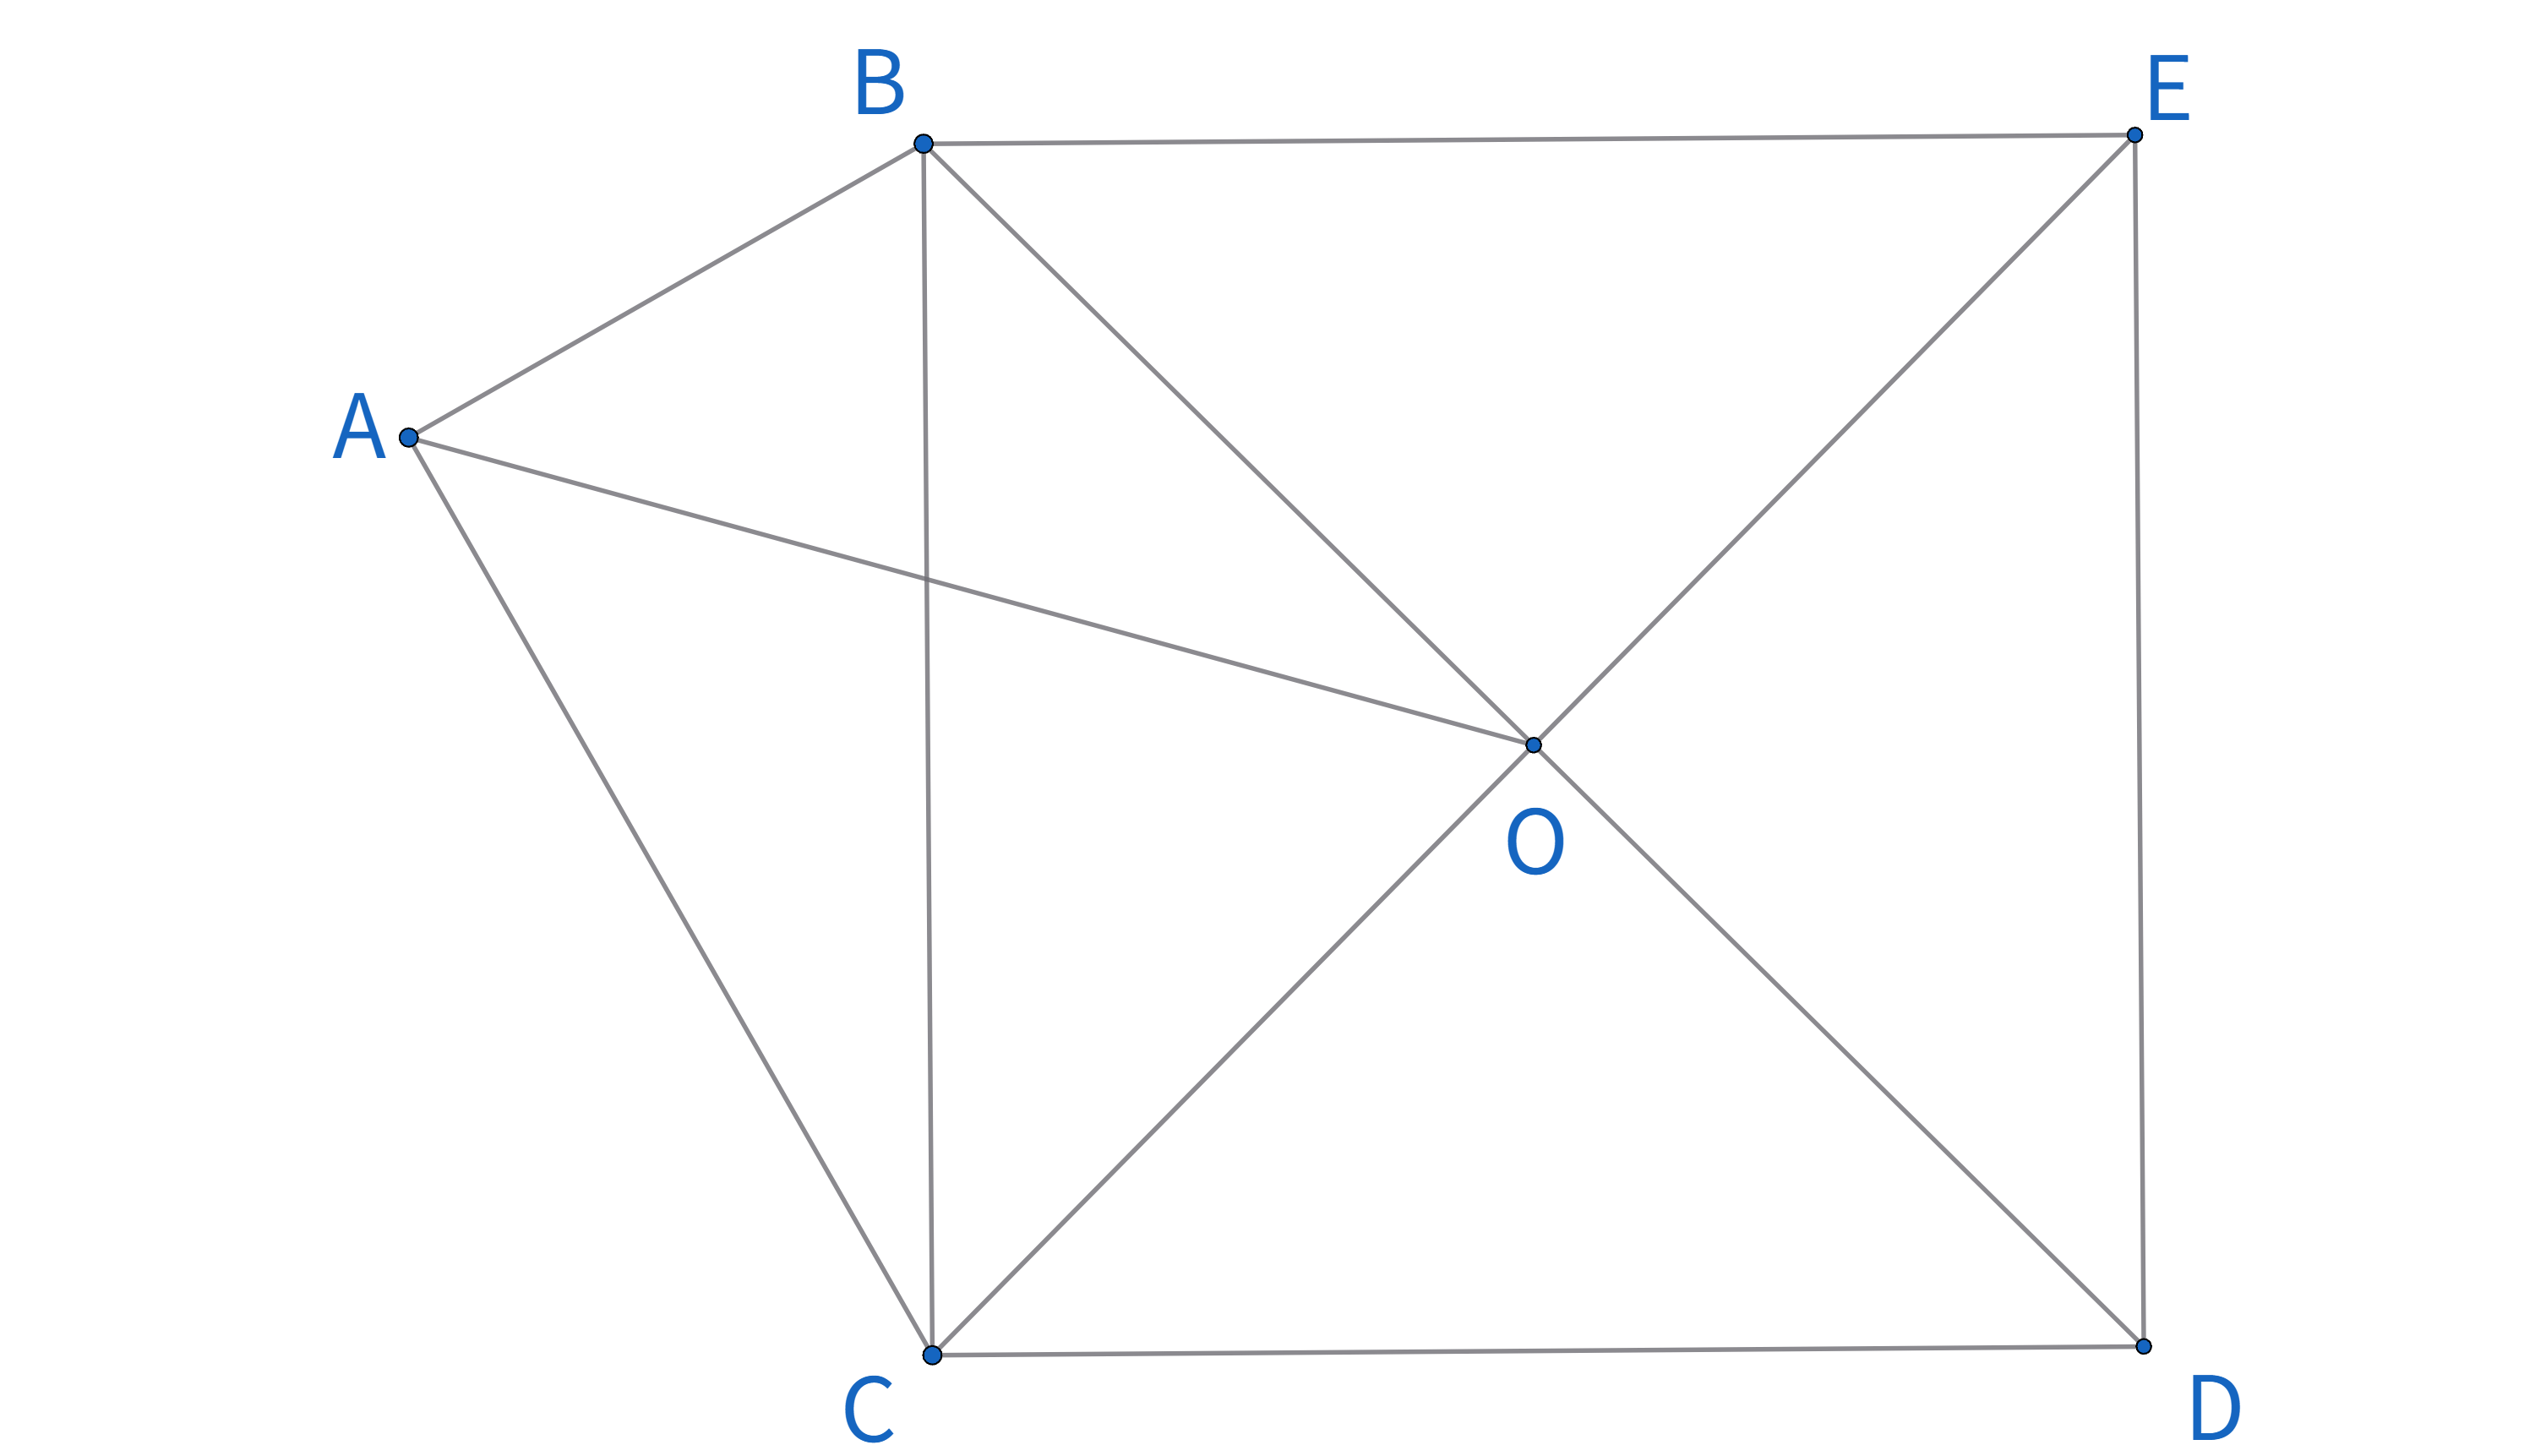
\includegraphics[width=0.7\linewidth]{figures/exercises/004.png}
\end{figure}


\newpage 
\section{蝴蝶定理}
\begin{theorem}
    设M为圆内弦PQ的中点,过M作弦AB和CD。设AD和BC各相交PQ弦于点X和Y,则M是XY的中点。
\end{theorem}

\begin{figure}[H]
    \centering
    \hfill % 添加一些水平间距
    \begin{minipage}[t]{0.45\textwidth}
    \centering
    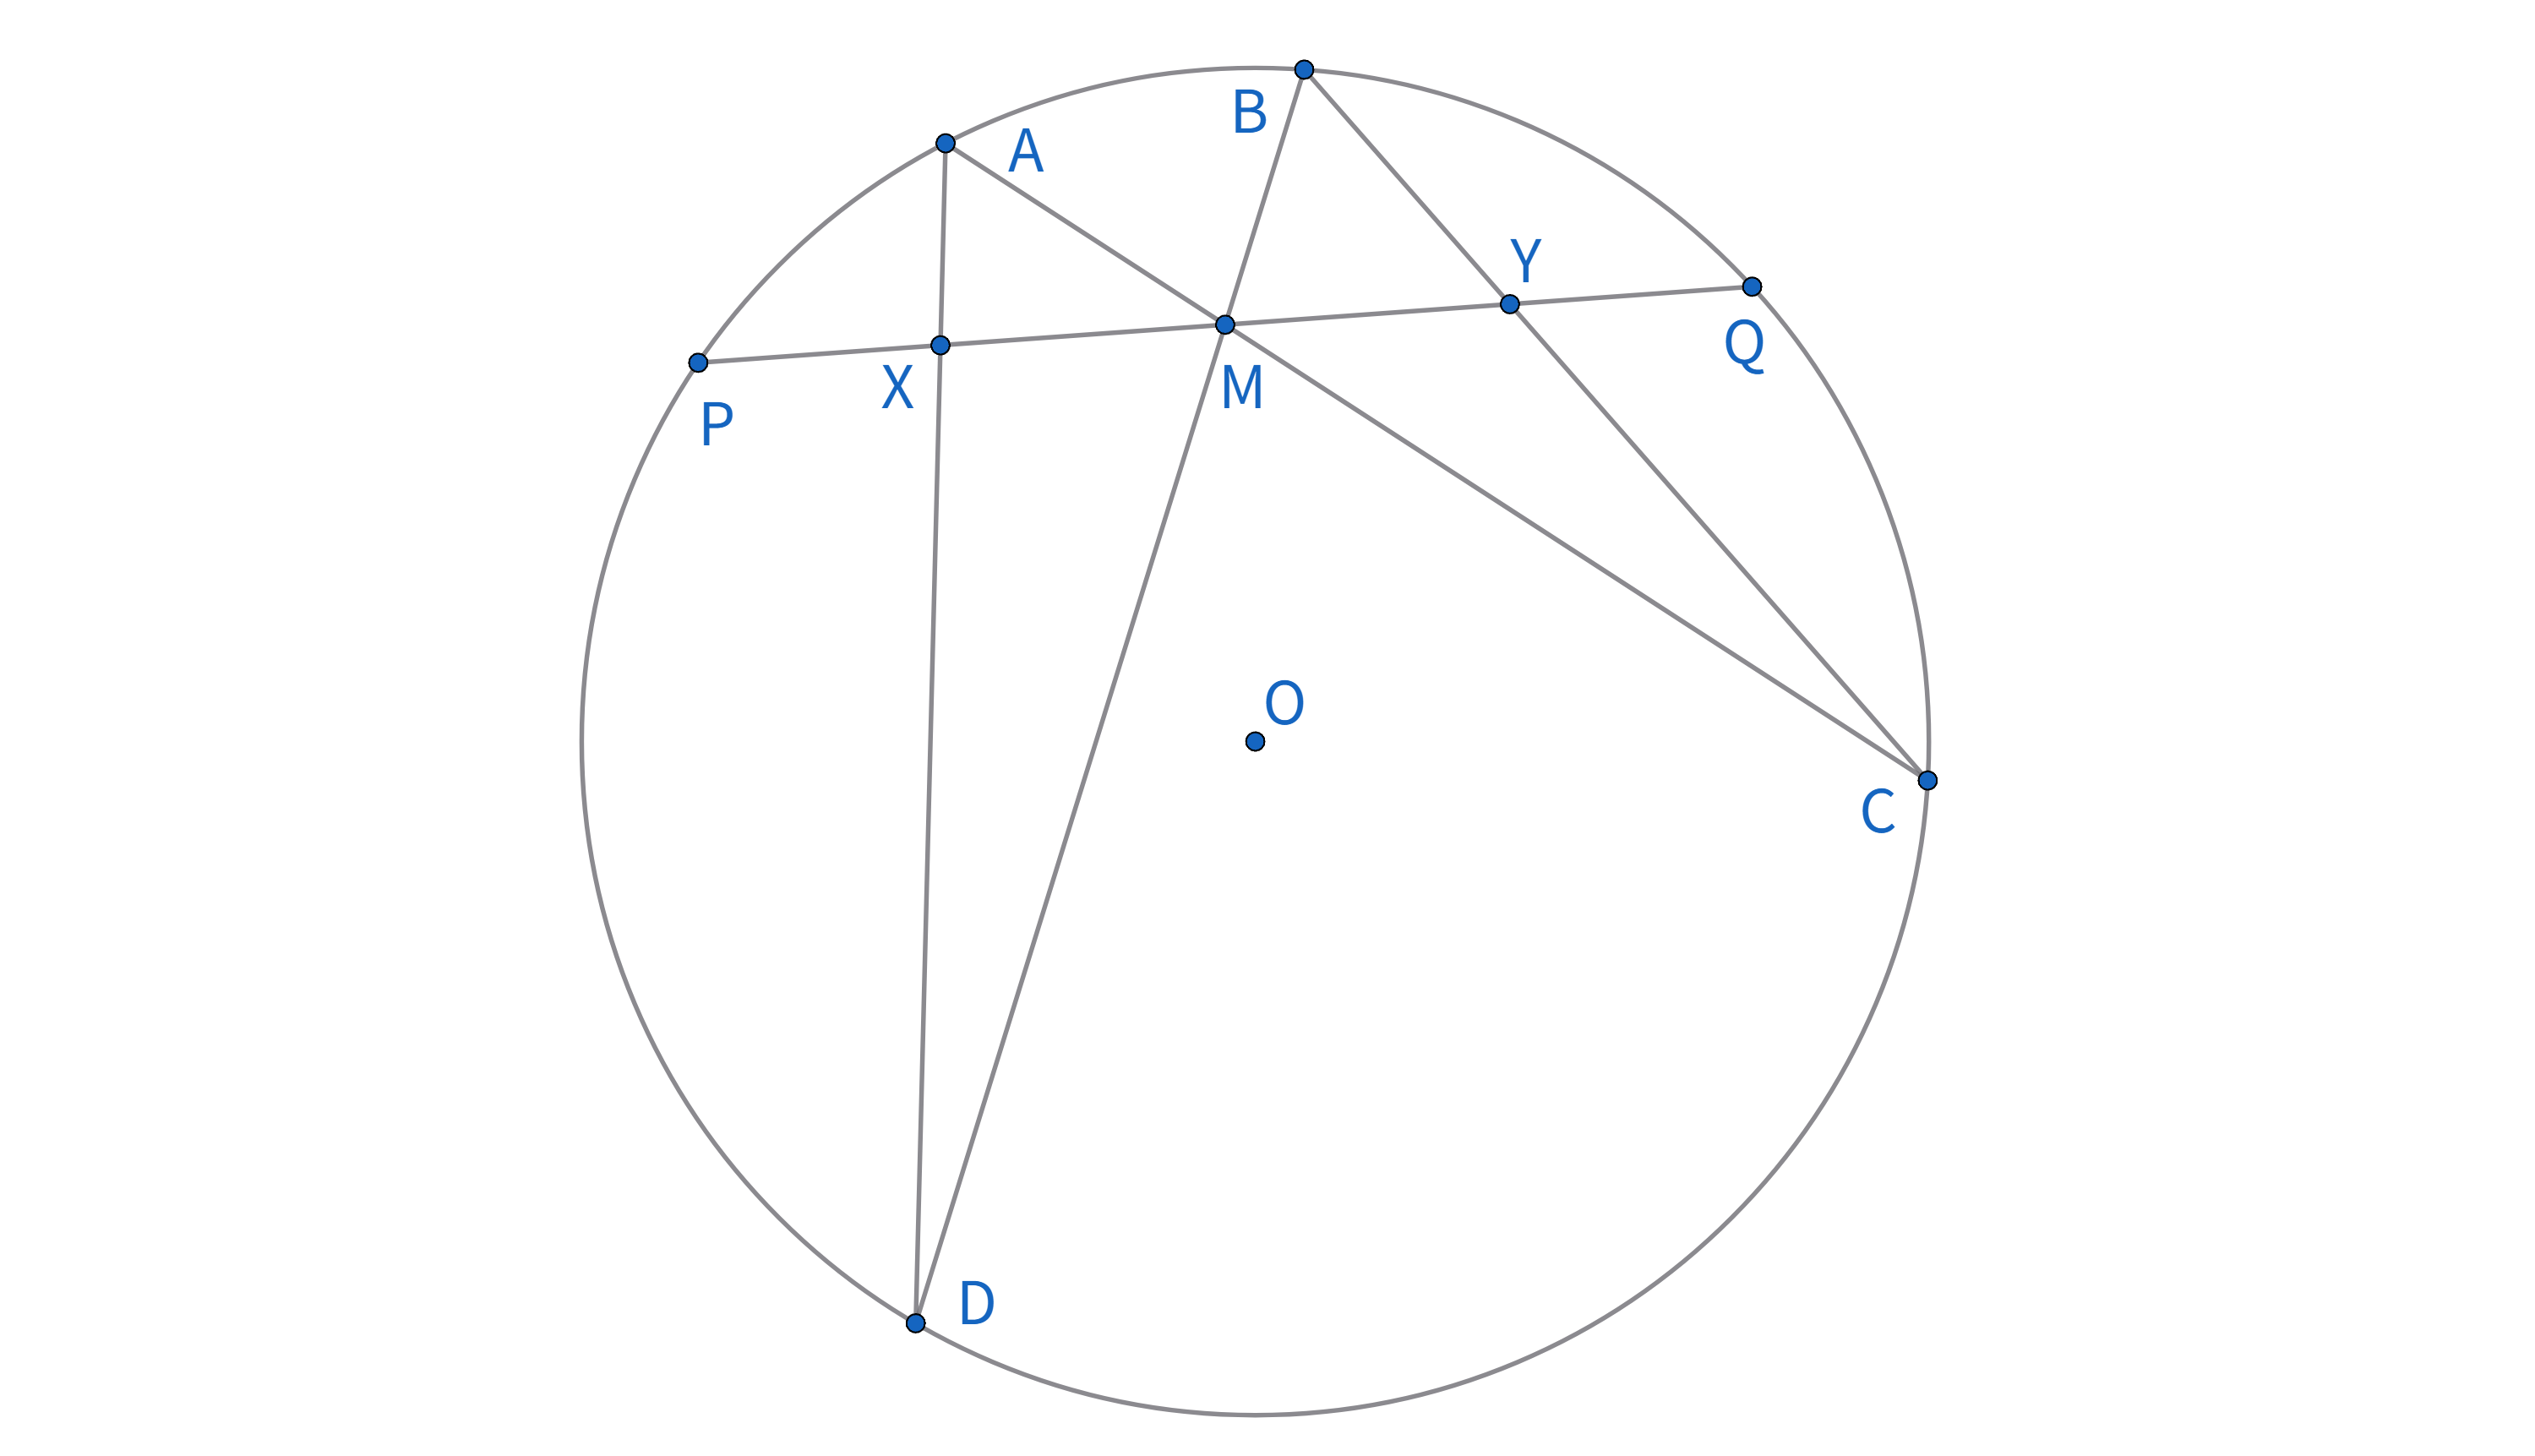
\includegraphics[width=\linewidth]{figures/蝴蝶定理.png}
    \end{minipage}
    \hfill % 添加一些水平间距
    \begin{minipage}[t]{0.45\textwidth}
    \centering
    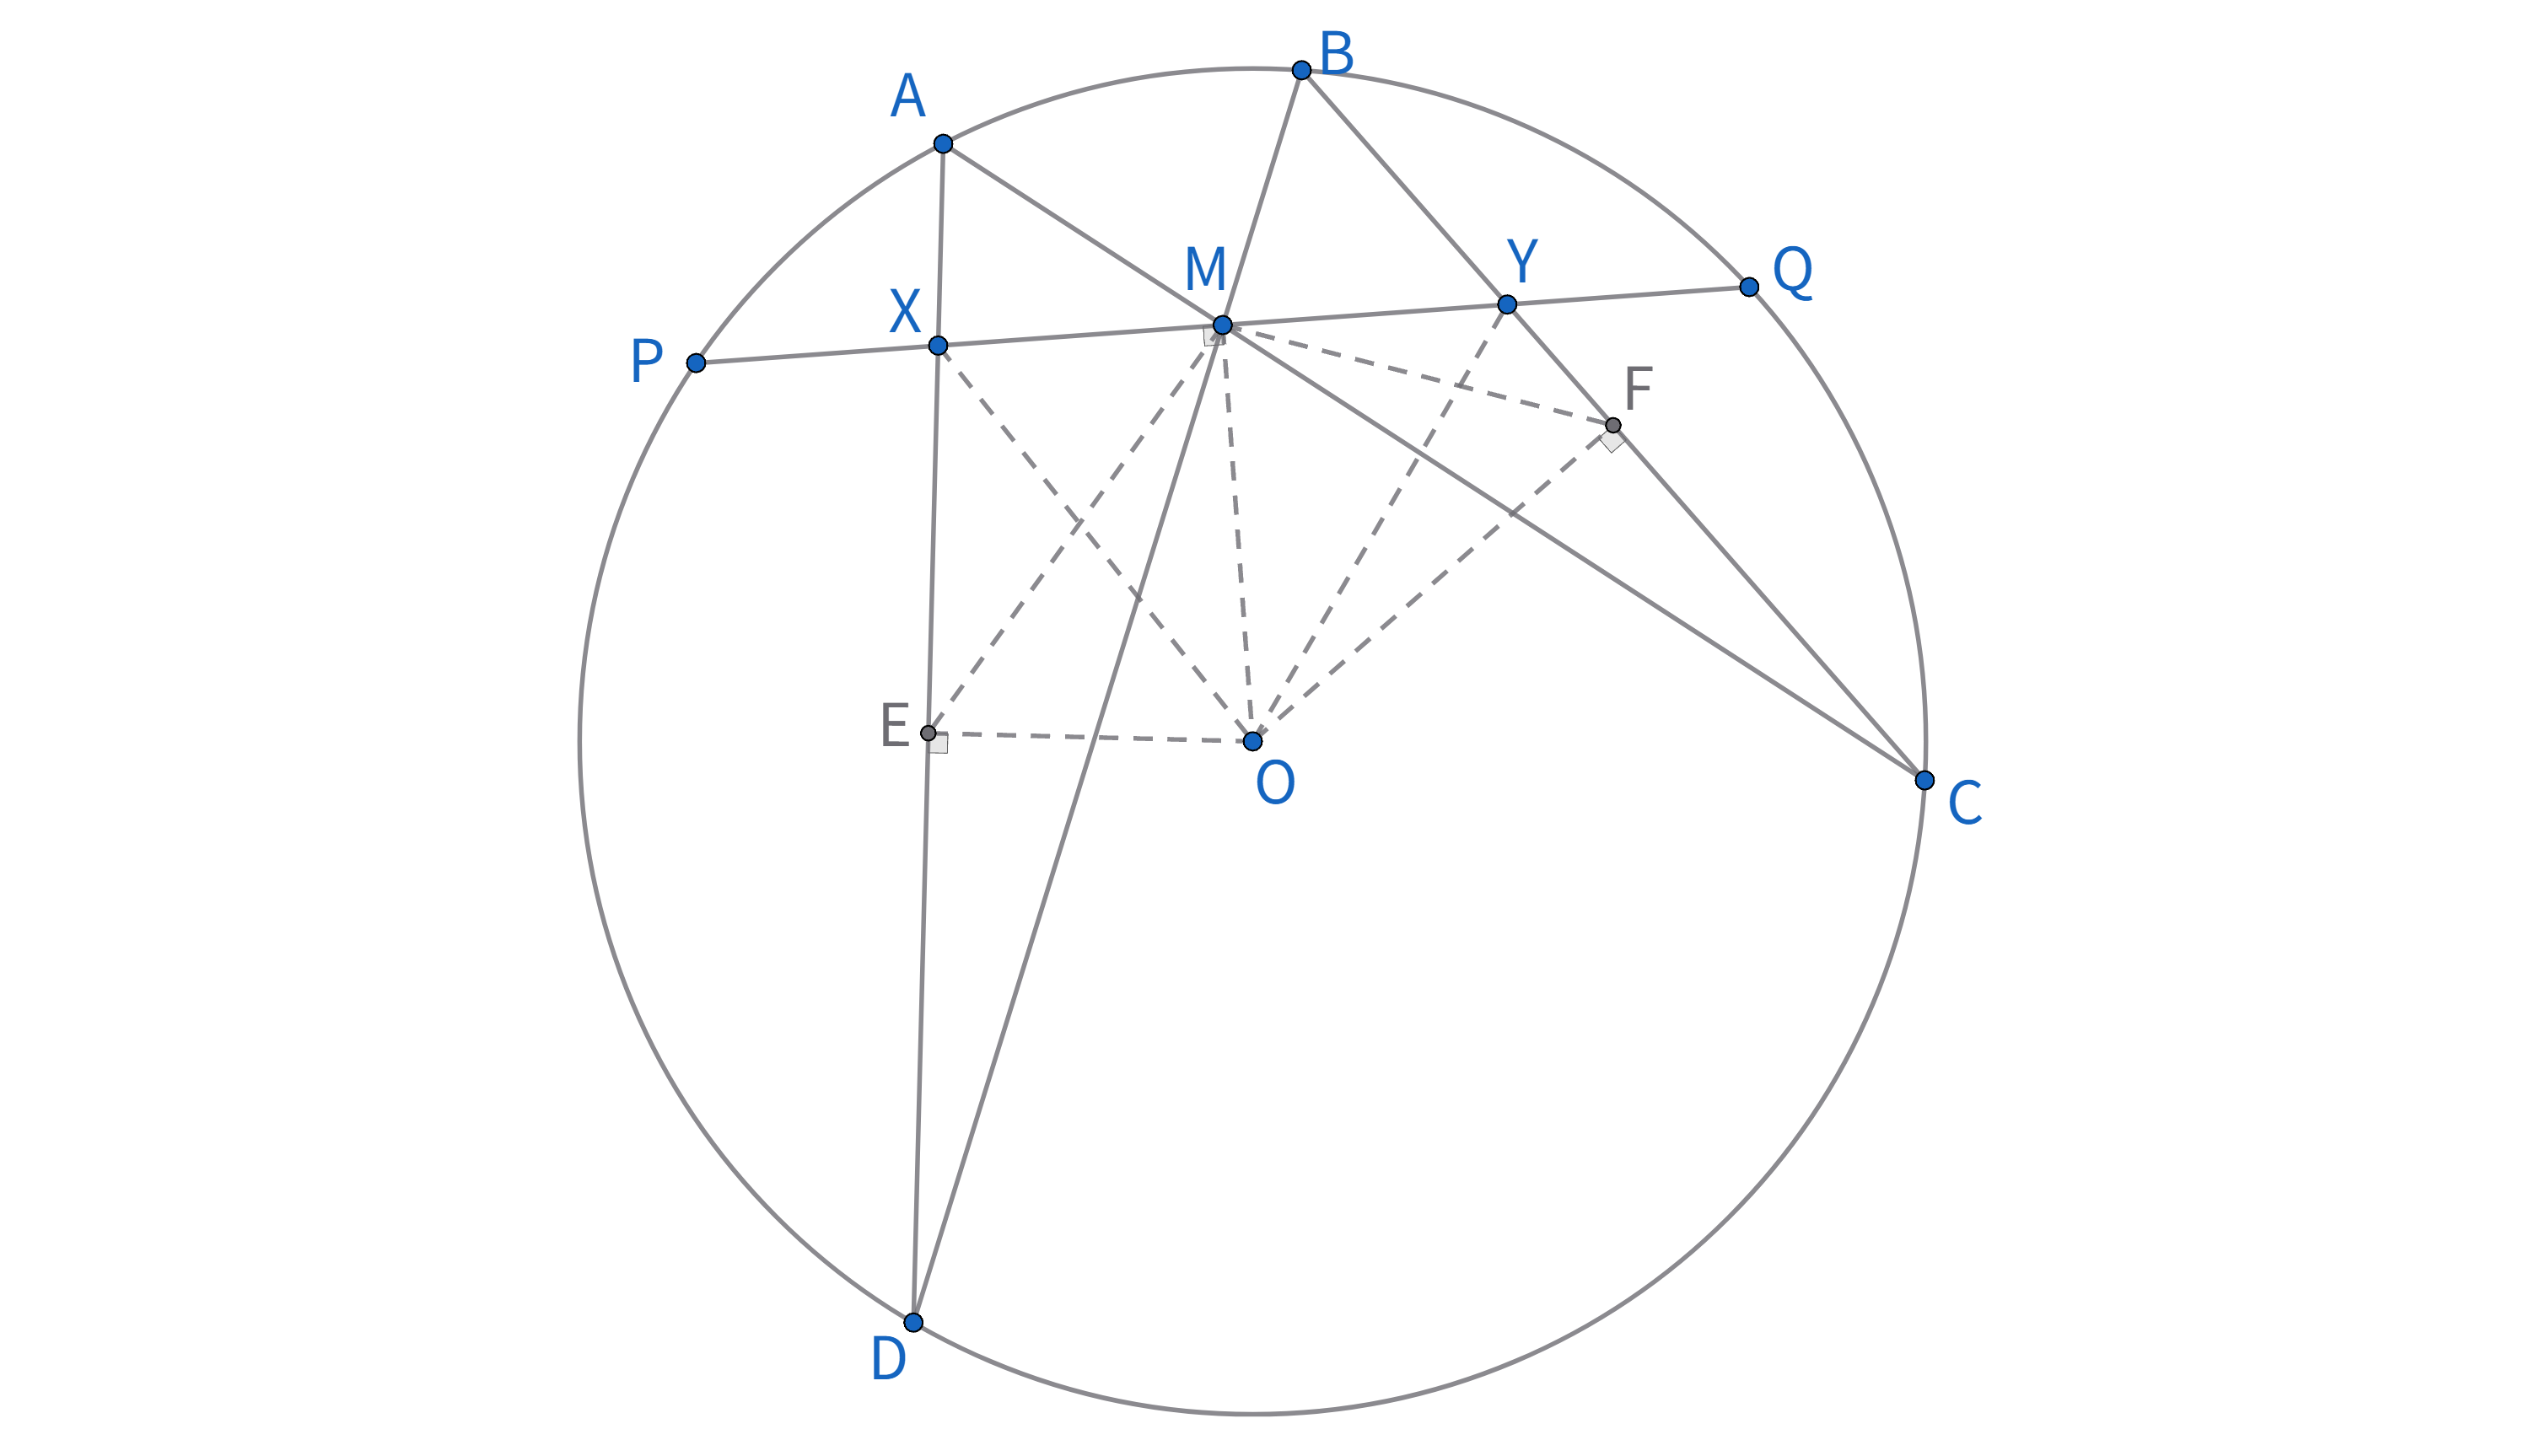
\includegraphics[width=\linewidth]{figures/蝴蝶定理辅助线.png}
    \end{minipage}
\end{figure}


\newpage 
\section{托勒密(Ptolemy)定理}
\begin{theorem}
    圆的内接四边形对角线乘积等于两组对边乘积之和。
    $$AC \cdot BD = AB \cdot CD + BC \cdot AD.$$
\end{theorem}
\begin{figure}[H]
    \centering
    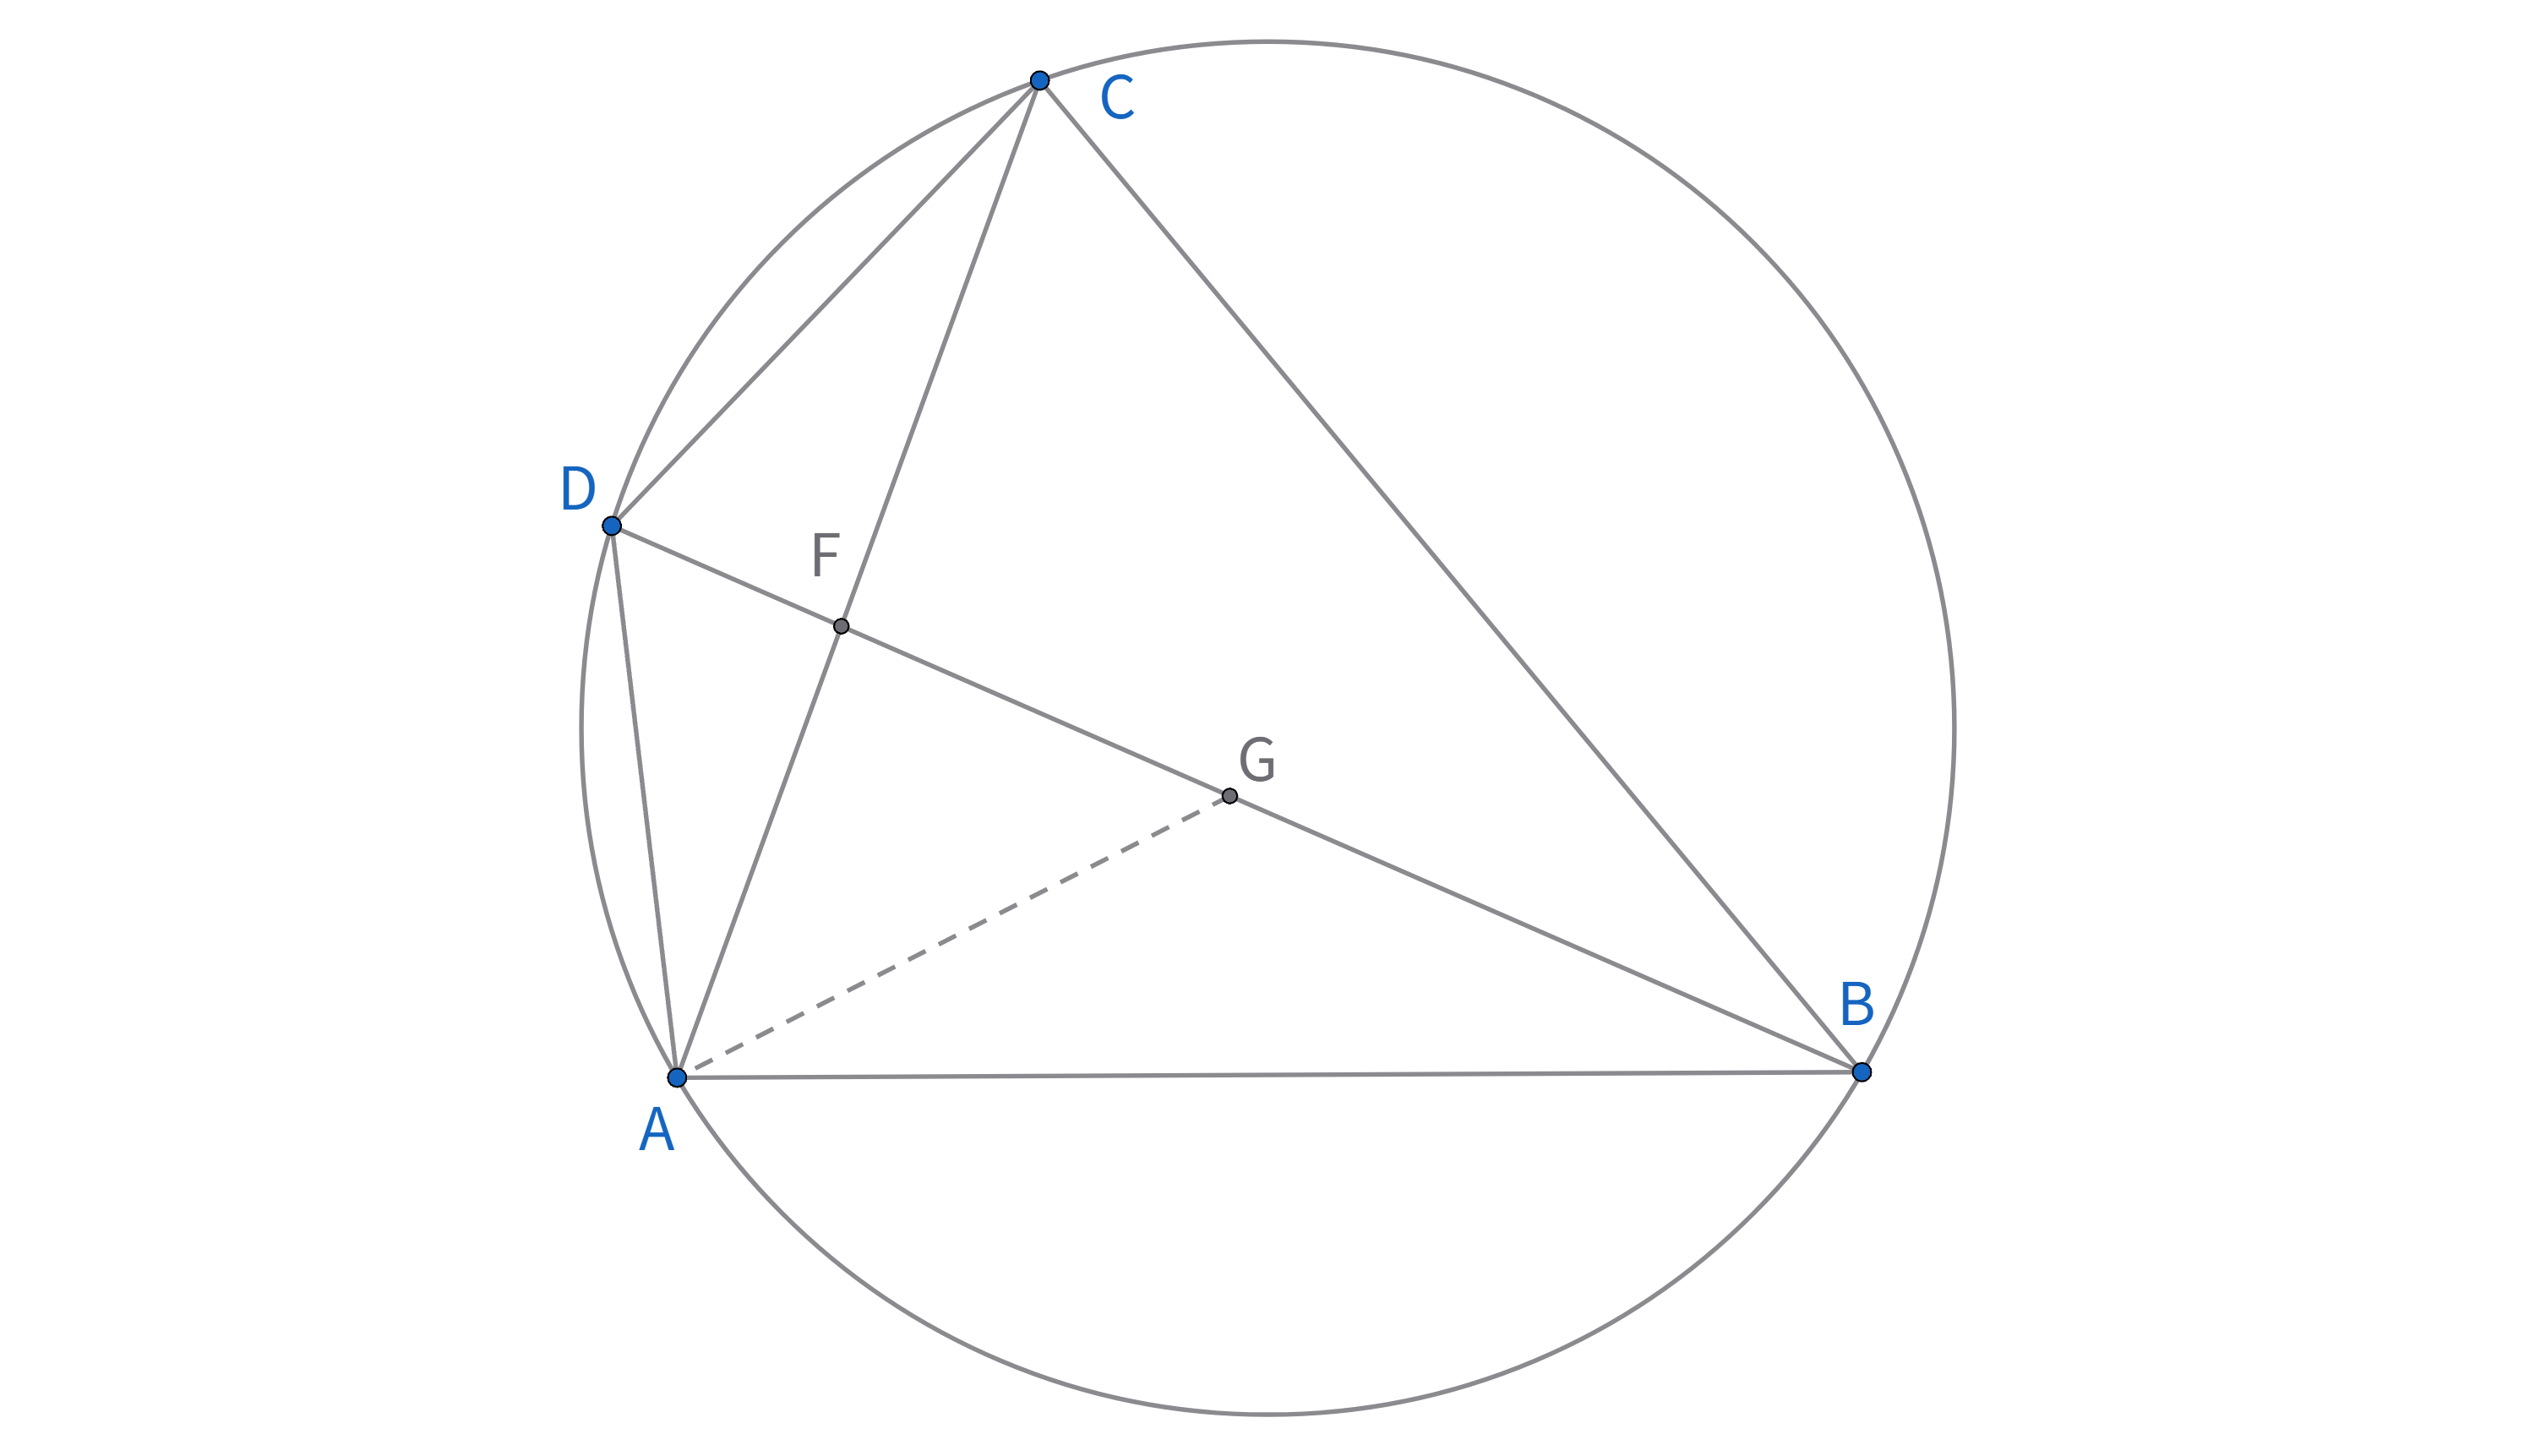
\includegraphics[width=0.7\linewidth]{figures/托勒密定理.png}
    \caption{托勒密定理}
\end{figure}
